\documentclass[12pt, a4paper, twoside, openright]{report}
\usepackage{hyphenat}

% --------------------------------------------------------
% Packages & Document Configuration
% --------------------------------------------------------

% Handling encodings and languages
\usepackage[utf8]{inputenc}
\usepackage[T1]{fontenc}
\usepackage{lmodern}
\usepackage[english]{babel}
\usepackage{csquotes}
% Standard margins for a thesis (left margin larger for physical binding)
\usepackage[left=1in, right=1in, top=1in, bottom=1in]{geometry}

% Line spacing (1.5 spacing is standard for theses)
\usepackage{setspace}
\onehalfspacing
\raggedbottom

% Image and figure support
\usepackage{graphicx}
\graphicspath{{images/}}  % Directory where Overleaf will look for images
\usepackage{caption}
\usepackage{subcaption}   % For side-by-side images

% Math, symbols, and formatting
\usepackage{amsmath}
\usepackage{amssymb}
\usepackage{microtype}    % Improves typographic layout
\usepackage{algorithmic}
% Table of contents and hyperlinks
\usepackage[colorlinks=true, linkcolor=black, citecolor=blue, urlcolor=blue]{hyperref}

\usepackage[backend=biber, style=ieee, sorting=none]{biblatex}
\addbibresource{references.bib}

\begin{document}

\pagenumbering{roman}

% --- Title Page ---
\begin{titlepage}
    \centering
    \vspace*{1.5cm}

    
\includegraphics[width=0.2\textwidth]{unipi_logo.png}\\
    {\large{\textsc{University of Pisa}}}\\
    {Department of Computer Science \\ Master Degree Programme in Computer Science and Networking}\\[1.5cm]

    {Master Thesis}\\
    {\bfseries A Heuristic Approach to Routing and Spectrum Assignment in Multi-Fiber Elastic Optical Networks: Design and Implementation in TeraFlowSDN}\\[2cm]


    \begin{minipage}[t]{0.4\textwidth}
        \raggedright
        \emph{Supervisors:} \\
        Prof. Alessio Giorgetti\\
        Dott. Andrea Sgambelluri\\
        Prof. Stefano Giordano
    \end{minipage}
    \hfill
    \begin{minipage}[t]{0.4\textwidth}
        \raggedleft
        \emph{Candidate:}\\
        ASM Chafiullah Bhuiyan
    \end{minipage}\\[2.5cm]

    {\large Academic Year: 2025-2026}\\[1.5cm]

    \vfill
\end{titlepage}

% --- Acknowledgements ---
\chapter*{Acknowledgements}
\addcontentsline{toc}{chapter}{Acknowledgements}
First and foremost, I would like to express my deepest gratitude to my primary supervisor, Professor Alessio Giorgetti and co-supervisors Dott. Andrea Sgambelluri, Prof. Stefano Giordano. I am incredibly thankful for their unwavering support, specifically my primary supervisor's willingness to share his resources, and for granting me welcoming access to his valuable time for discussions. His generous investment of valuable time and expertise was instrumental in allowing me to complete this extensive and complex project within the given timeframe. Furthermore, I am deeply appreciative of his provision of dedicated hardware resources, which afforded me endless opportunities to conduct rigorous testing and successfully validate my work.

Finally, words cannot adequately express my profound gratitude to my family for their immense sacrifices during my time studying abroad. I owe a special and heartfelt thank you to my children, who have had to navigate a significant part of their childhood missing their father. Your love, patience, understanding, and resilience have been my greatest source of strength and motivation throughout this journey. This thesis is as much yours as it is mine.

% --- Abstract ---
\chapter*{Abstract} \addcontentsline{toc}{chapter}{Abstract} The provisioning of lightpaths in Flex-grid Elastic Optical Networks (EONs) significantly improves spectrum utilization, but introducing multiple parallel links between optical devices makes Routing and Spectrum Assignment (RSA) highly complex. When devices like transponders and Reconfigurable Optical Add-Drop Multiplexers (ROADMs) connect through multiple parallel fibers, the number of possible routing paths increases exponentially. Traditional Software-Defined Networking (SDN) controllers struggle to process this volume of paths efficiently. This challenge is further complicated by the ITU-T G.694.1 spectrum continuity and contiguity constraints; the controller must continuously verify the availability of specific flex-grid slots across all possible links to ensure the signal uses the same uninterrupted frequency end-to-end.

To solve these bottlenecks in path scalability and spectrum mapping, this thesis introduces the ParallelOpticalController (POC), a novel microservice integrated directly into the TeraFlowSDN (TFS) ecosystem. The controller constructs a multi-directed graph $G$ using the NetworkX library that natively supports parallel edges, and then collapses it into a simplified graph $G_s$ where parallel links are abstracted into single logical edges. This structural simplification reduces routing complexity from exponential to linear in the number of parallel links, allowing Dijkstra's algorithm to compute the shortest path on $G_s$ while concurrently discovering alternative path combinations to minimize blocking probabilities. The selected node-level path is subsequently expanded back onto $G$ via an in-memory lookup table, recovering all parallel link combinations without re-traversing the full topology. To reduce the heavy spectrum calculation overhead, the controller employs a bitmap-based bitwise intersection method. By aligning heterogeneous endpoint frequency ranges to a standardized reference and performing mathematical intersections of available slots across sequential hops, it rapidly identifies contiguous spectrum blocks. Additionally, the existing TFS \emph{OpenConfig} and \emph{OpenROADM} device drivers are enhanced with a dynamically adaptable extraction technique that applies device-model-specific filter profiles, and the TFS WebUI is comprehensively upgraded to visualize real-time spectrum availability and optical connectivity.

To assess performance, the heuristic is evaluated across three reference topologies---Linear, \textit{NSFNET}, and \textit{PANEU}---each configured in both single-link and parallel-link variants. The computational efficiency metric, defined as the ratio of single-link to parallel-link execution time, peaks at 91.54\% for the PANEU parallel configuration (27 nodes, 165 links), demonstrating that the graph abstraction technique successfully insulates pathfinding from increased spatial complexity. The controller sustains a throughput of up to 300 requests per second in baseline configurations and maintains robust provisioning rates even under dense multi-fiber scenarios. The statistical analysis is performed with several path selection schemes within the set of shortest paths (SP): first-fit (SPFF), random-fit (SPRF), and spectrum-check (SPSC). Regarding the spectrum assignment (SA), the first-fit (SAFF) policy is adopted as the primary approach. The simulation results demonstrate that the SPSC scheme consistently achieves superior performance. Analysis of the NSFNET topology at $250$ Erlangs reveals that the SPSC scheme maintains a blocking probability below $10^{-4}$, whereas SPFF and SPRF typically range between $10^{-3}$ and $10^{-4}$. For the PANEU topology, the SPSC scheme achieves blocking probabilities between $10^{-3}$ and $10^{-4}$, outperforming the NSFNET equivalent which ranges between $10^{-2}$ and $10^{-3}$ at comparable loads. The results remain consistent in topologies featuring three parallel links under network loads scaled by a factor of three.


% --- Tables of Contents, Figures, and Tables ---
\tableofcontents
\clearpage
\listoffigures
\addcontentsline{toc}{chapter}{\listfigurename}
\clearpage
\listoftables
\addcontentsline{toc}{chapter}{\listtablename}
\chapter*{Glossary}
\addcontentsline{toc}{chapter}{Glossary}

\begin{description}
    \item[CWDM] Coarse Wavelength Division Multiplexing
    \item[DEG] Degree (block within a ROADM)
    \item[DSL] Digital Subscriber Line
    \item[DSP] Digital Signal Processor
    \item[DSP (Dijkstra)] Dijkstra's Shortest Path
    \item[DWDM] Dense Wavelength Division Multiplexing
    \item[EDFA] Erbium-Doped Fiber Amplifier
    \item[EON] Elastic Optical Network
    \item[ETSI] European Telecommunications Standards Institute
    \item[FSU] Frequency Slot Unit
    \item[FTTH] Fiber-to-the-Home
    \item[GG] Graph Generation
    \item[GMPLS] Generalized Multiprotocol Label Switching
    \item[GNPy] Gaussian Noise model in Python
    \item[gRPC] Google Remote Procedure Calls
    \item[ILP] Integer Linear Programming
    \item[IPoDWDM] IP over Dense Wavelength Division Multiplexing
    \item[ITU] International Telecommunication Union
    \item[JSON] JavaScript Object Notation
    \item[K8s] Kubernetes
    \item[LCoS] Liquid Crystal on Silicon
    \item[MDP] Markov Decision Process
    \item[MEC] Multi-access Edge Computing
    \item[MHLS] Minimum Hops with Least Slots
    \item[MSC] Maximum Spectrum Completeness
    \item[NAT] Network Address Translation
    \item[NETCONF] Network Configuration Protocol
    \item[NFV] Network Function Virtualization
    \item[NSFNET] National Science Foundation Network
    \item[ODL] OpenDaylight
    \item[OEO] Optical-Electrical-Optical
    \item[ONOS] Open Network Operating System
    \item[PANEU] Pan-European (network topology)
    \item[POC] ParallelOpticalController (microservice)
    \item[QSFP-DD] Quad Small Form-factor Pluggable -- Double Density
    \item[QoT] Quality of Transmission
    \item[RDD] Resource Dependency Digraph
    \item[RESTCONF] Representational State Transfer Configuration Protocol
    \item[ROADM] Reconfigurable Optical Add-Drop Multiplexer
    \item[RSA] Routing and Spectrum Assignment
    \item[SA] Spectrum Assignment
    \item[SAC] Spectrum Assignment Computation
    \item[SAFF] Spectrum Assignment First-Fit
    \item[SARF] Spectrum Assignment Random-Fit
    \item[SDH] Synchronous Digital Hierarchy
    \item[SDN] Software-Defined Networking
    \item[SFP+] Enhanced Small Form-factor Pluggable
    \item[SNR] Signal-to-Noise Ratio
    \item[SONET] Synchronous Optical Networking
    \item[SP] Shortest Path
    \item[SPC] Shortest Path Computation
    \item[SPFF] Shortest Path First-Fit
    \item[SPRF] Shortest Path Random-Fit
    \item[SPSC] Shortest Path Spectrum Check
    \item[SRG] Shared Risk Group
    \item[T-API] Transport Application Programming Interface
    \item[TFS] TeraFlowSDN
    \item[WDM] Wavelength Division Multiplexing
    \item[WSON] Wavelength Switched Optical Network
    \item[WSS] Wavelength Selective Switch
    \item[YANG] Yet Another Next Generation (data modeling language)
\end{description}

% --- Main Body ---
\clearpage
% Switch back to Arabic numbering (1, 2, 3...) for the main text
\pagenumbering{arabic}

% --- Introduction ---
\chapter{Introduction}
\section{Internet in Modern Era}
In 2025, approximately 6 billion people use the internet, and this accounts for nearly 74\% of the global population~\cite{ituInternetUse}. While mobile broadband traffic is growing rapidly, fixed networks still carry the vast majority of global data~\cite{ituInternetTraffic}. This immense data flow is driven by modern digital applications, which demand continuous and high-bandwidth data transmission. High-definition video conferencing requires highly stable connectivity, whereas cloud-based gaming strictly demands low-latency data transfer. Additionally, the widespread deployment of connected sensors generates heavy uplink traffic, because live security surveillance operates continuously around the clock.

Furthermore, recent advancements in artificial intelligence have altered network demands, and these technologies introduce highly unpredictable traffic patterns~\cite{nokiaProjection}. The distributed training of large machine learning models requires massive data synchronization, which frequently causes sudden traffic bursts across data centers. As machine-to-machine communications expand globally, overall data volumes are projected to maintain a steep upward trajectory. Satisfying this escalating demand requires robust infrastructure, but accommodating such immense scale was not always possible in the past. The capacity to sustain today's interconnected world relies on fundamental physical transformations, which defined the historical evolution of communication networks.

\subsection{Evolution of the Network}
To accommodate massive traffic growth, communication networks have undergone significant technological breakthroughs across all core and edge segments. In the access network, traditional copper-based Digital Subscriber Line (DSL) and xDSL technologies face severe bandwidth limitations. Consequently, they are being replaced by Fiber-to-the-Home (FTTH) architectures, which deliver optical fiber directly to user premises. Additionally, the widespread deployment of 5G mobile networks provides high-speed wireless access, and this requires dense optical fiber backhaul to function effectively. In the metro segment, older standards like Synchronous Optical Networking (SONET) and Synchronous Digital Hierarchy (SDH) have become obsolete. Providers have replaced them with Wavelength Division Multiplexing (WDM) metro rings, which utilize highly scalable Ethernet interfaces. Similarly, the backbone segment has transitioned from SONET/SDH to Wavelength Switched Optical Networks (WSONs). In these advanced networks, traffic is switched entirely within the optical domain, and this eliminates the need for slow Optical-Electrical-Optical (OEO) conversions at intermediate nodes. Therefore, routing is determined by the physical wavelength of the signal rather than electrically processed binary information.

This structural evolution is driven by fundamental physical limits in data transmission. Traditional electronic transmission operating in the gigahertz (GHz) spectrum is rapidly approaching its maximum capacity limit. Because sudden data growth frequently exhausts this available bandwidth, terahertz (THz) transmission is emerging as the necessary standard for next-generation networks. Operating in the THz optical spectrum allows fibers to support immense data throughput. However, to fully exploit this massive bandwidth over a single physical medium, optical networks rely heavily on parallel transmission technologies. The foundational technique that enables this multi-channel communication is WDM.

\subsection{Wavelength Division Multiplexing}
WDM revolutionized optical networks, because it enables the simultaneous transmission of multiple distinct data channels over a single physical fiber. As we can see in Fig.~\ref{fig:wdm_transmission}, multiple wavelengths transmitted from a transponder are combined together by the optical multiplexer and transmitted to the next point ì. This capability drastically increased overall network capacity, and it eliminated the massive costs associated with deploying new fiber cables. WDM systems are broadly categorized into Coarse WDM (CWDM) and Dense WDM (DWDM). CWDM utilizes wider channel spacing, and it provides a cost-effective solution for short-distance metropolitan or enterprise networks. Conversely, DWDM minimizes channel spacing to pack numerous wavelengths tightly together, which makes it essential for high-capacity, long-haul backbone networks.
\begin{figure}[htbp]
    \centering
    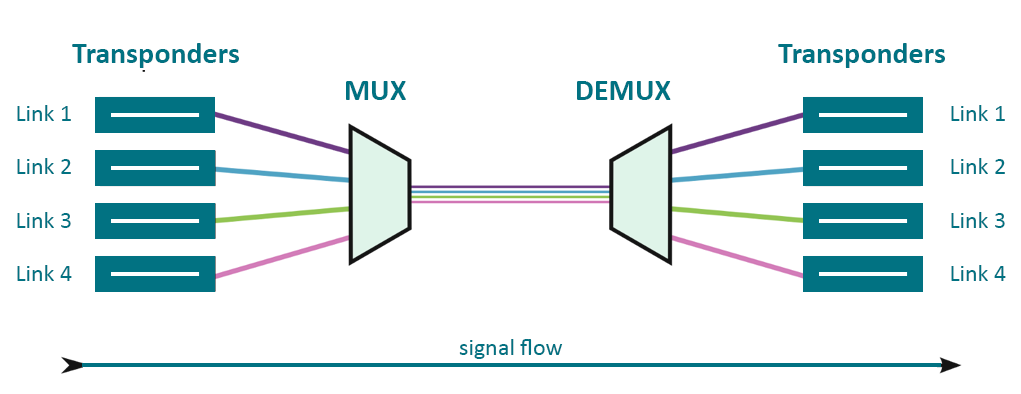
\includegraphics[width=0.8\textwidth]{cover-wdm-.png}
    \caption{Optical Transmission using WDM}
    \label{fig:wdm_transmission}
\end{figure}
Early DWDM deployments utilized a fixed-grid frequency allocation, which strictly divided the optical spectrum into~\emph{50GHz} rigid channels of equal size. However, fixed-grid architectures became highly inefficient, because they waste valuable spectral resources when transmitting modern, heterogeneous data rates. Consequently, flex-grid DWDM emerged as the modern industry standard, as it dynamically allocates spectrum in granular, variable-sized frequency slices where the spectrum is divided into~\emph{12.5GHz} rigid channels. This flex-grid paradigm forms the technological foundation of Elastic Optical Networks (EONs). As illustrated in Fig.~\ref{fig:example_usage_of_flex_grid} EONs adaptively assign precise optical bandwidth based on actual traffic demands, and this operational flexibility maximizes the overall spectral efficiency of the fiber.

\begin{figure}[htbp]
    \centering
    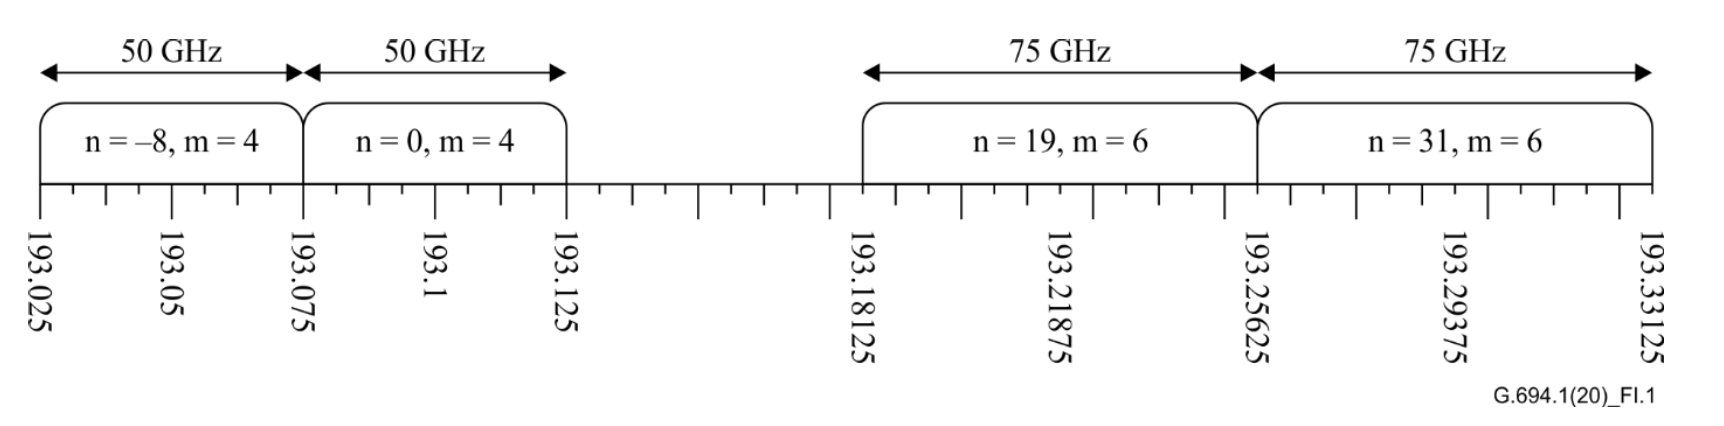
\includegraphics[width=0.8\textwidth]{example_of_flex_grid.png}
    \caption{Elastic Optical Network~\cite{itu694}}
    \label{fig:example_usage_of_flex_grid}
\end{figure}

Operating these dynamic networks requires sophisticated optical hardware components. Routing is handled by Wavelength Selective Switches (WSS), which dynamically direct specific wavelengths across the network without electrical conversion. Modern WSS components utilize Liquid Crystal on Silicon (LCoS) technology, and this enables highly precise, software-controlled manipulation of the optical spectrum. To overcome signal attenuation over long distances, Erbium-Doped Fiber Amplifiers (EDFAs) boost the multiplexed light signals entirely within the optical domain. While EDFAs ensure sufficient signal reach, the transmission of massive data rates through densely packed optical channels introduces severe physical signal distortions. Overcoming these complex optical impairments requires highly advanced transceiver technologies. To address this fundamental challenge, modern networks mandate the use of coherent optics.
\subsection{Coherent Optics}
In a traditional optical network, data traffic originates at edge or core IP routers, and it flows toward dedicated optical transponders. These transponders convert standard electrical client signals into specific DWDM wavelengths, and they subsequently forward the traffic to ROADMs for long-distance optical routing. The optical conversion is executed by coherent pluggable transceivers~\ref{fig:optical-transceivers}, which are plugged directly within the transponder line cards. The internal architecture of a coherent module typically integrates a Digital Signal Processor (DSP), a tunable laser, and advanced optical modulators. This specific design allows precise tunability across multiple optical frequencies, which provides immense operational flexibility for network administrators.
\begin{figure*}[t]
    \centering
    \begin{subfigure}[b]{0.38\textwidth}
        \centering
        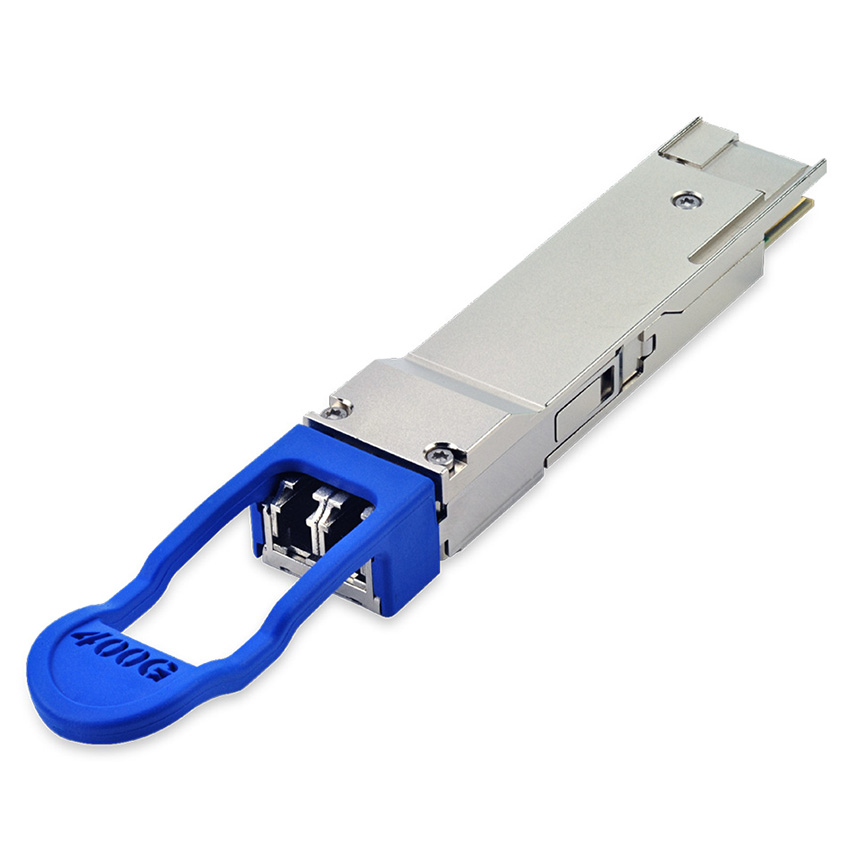
\includegraphics[width=\textwidth]{optical-transceivers.jpg}
        \caption{}
        \label{fig:optical-transceivers}
    \end{subfigure}
    \hfill
    \begin{subfigure}[b]{0.58\textwidth}
        \centering
        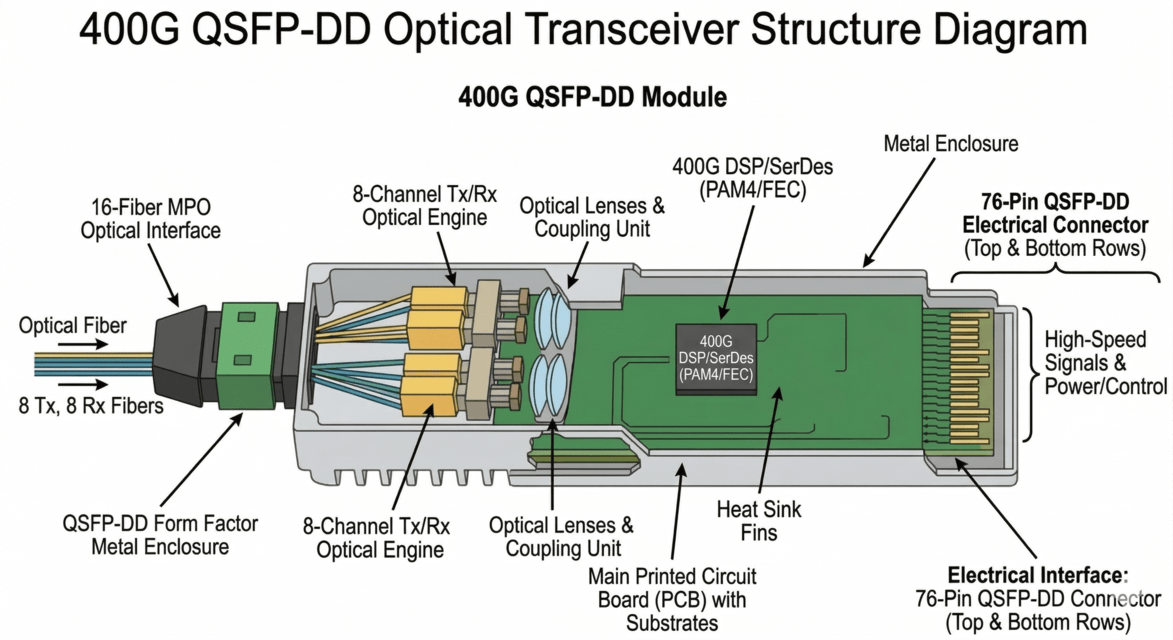
\includegraphics[width=\textwidth]{qsfp-dd-400G.png}
        \caption{}
        \label{fig:qsfp-dd-400G}
    \end{subfigure}
    \caption{(a) Coherent pluggables (SFP+) and (b) Structure Diagram (QSFP-DD)}
    \label{fig:coherent-pluggables}
\end{figure*}
These miniaturized components offer significant cost-effectiveness, and they are frequently deployed in compact form factors like the QSFP-DD for standard 400G transmissions~\ref{fig:qsfp-dd-400G}. Furthermore, ongoing advancements in coherent digital signal processing are actively enabling massive 800G and 1.6T transmission rates. To further optimize network efficiency, many operators are now transitioning toward IP over DWDM (IPoDWDM) architectures. IPoDWDM entirely eliminates the need for intermediate transponder hardware, because the coherent transceivers are plugged directly into the IP routers.

While this router-integrated approach generally restricts transmissions to shorter regional distances, it significantly reduces capital expenditures and overall power consumption. Regardless of whether the light originates from a standalone transponder or an IPoDWDM router, these ultra-high-capacity coherent signals must be seamlessly directed across the physical fibers. Managing these data streams without electrical conversion requires specialized, dynamic switching infrastructure. In modern optical architectures, this complex wavelength routing is exclusively managed by Reconfigurable Optical Add-Drop Multiplexers (ROADMs).

\subsection{Reconfigurable Optical Add-Drop Multiplexers}
ROADMs utilize WSS to route optical channels, and these switches form the functional core of modern optical nodes. Inside the WSS, LCoS technology uses microscopic liquid crystals to dynamically steer specific light wavelengths. This precise manipulation allows the network to bypass electrical processing entirely, which significantly reduces data transmission latency. A standard OpenROADM architecture~\ref{fig:OpenROADMDevice} logically divides this node into Degree (DEG) blocks and Shared Risk Group (SRG) blocks. The DEG block manages the external line-side optical fibers, and it securely connects the local node to other ROADMs across the broader network. Conversely, the SRG block provides the critical add/drop functionality, where local transponder signals safely enter or exit the optical network.
\begin{figure}[htbp]
    \centering
    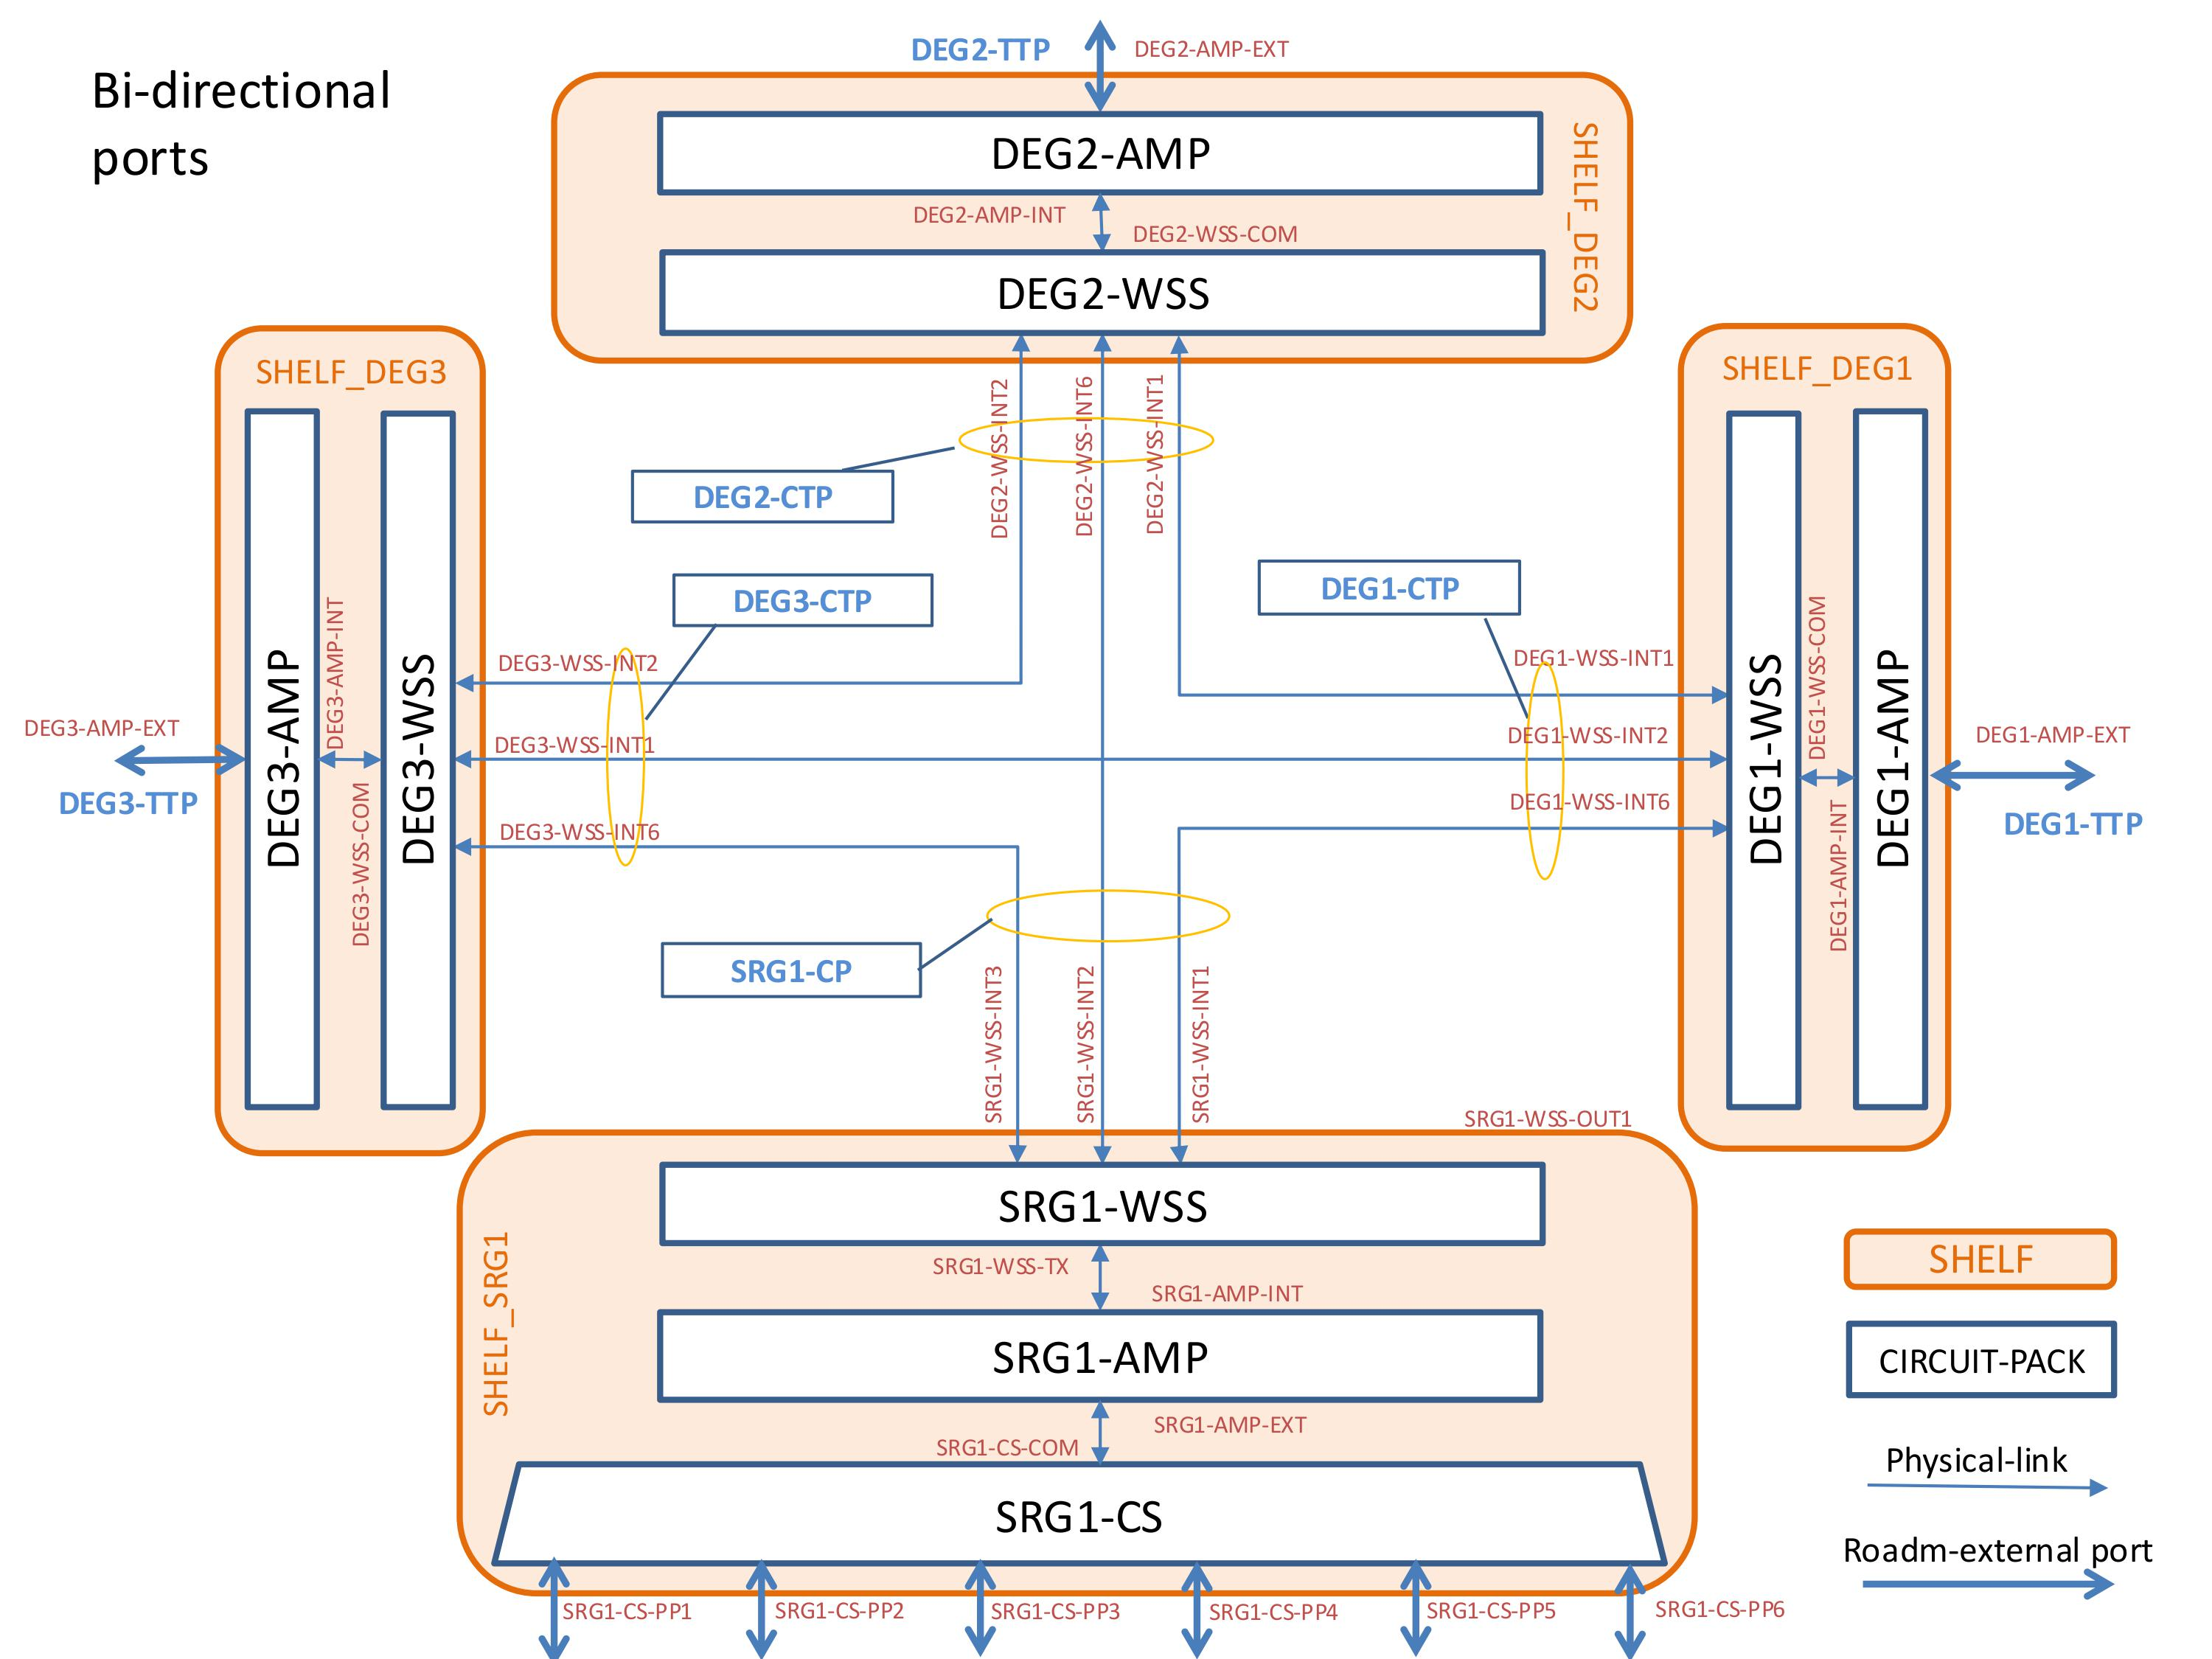
\includegraphics[width=0.8\textwidth]{OpenROADMDevice.jpg}
    \caption{OpenROADM Device for Metro-haul Connectivity}
    \label{fig:OpenROADMDevice}
\end{figure}
Internally, sophisticated optical cross-connects link the SRG components to the DEG components, and they also connect multiple DEGs together to seamlessly bypass local traffic. Externally, client transponders connect directly to the SRG ports, while long-haul fiber links connect one node's DEG to another node's DEG. When multiple physical links exist between two ROADM nodes, the network gains enhanced capacity and crucial path redundancy. Traffic can be dynamically balanced across these parallel links, or it can be instantly rerouted during unexpected failures. However, wavelength management within this architecture introduces specific physical constraints, and these constraints strictly dictate optical frequency reuse.
\begin{figure}[htbp]
    \centering
    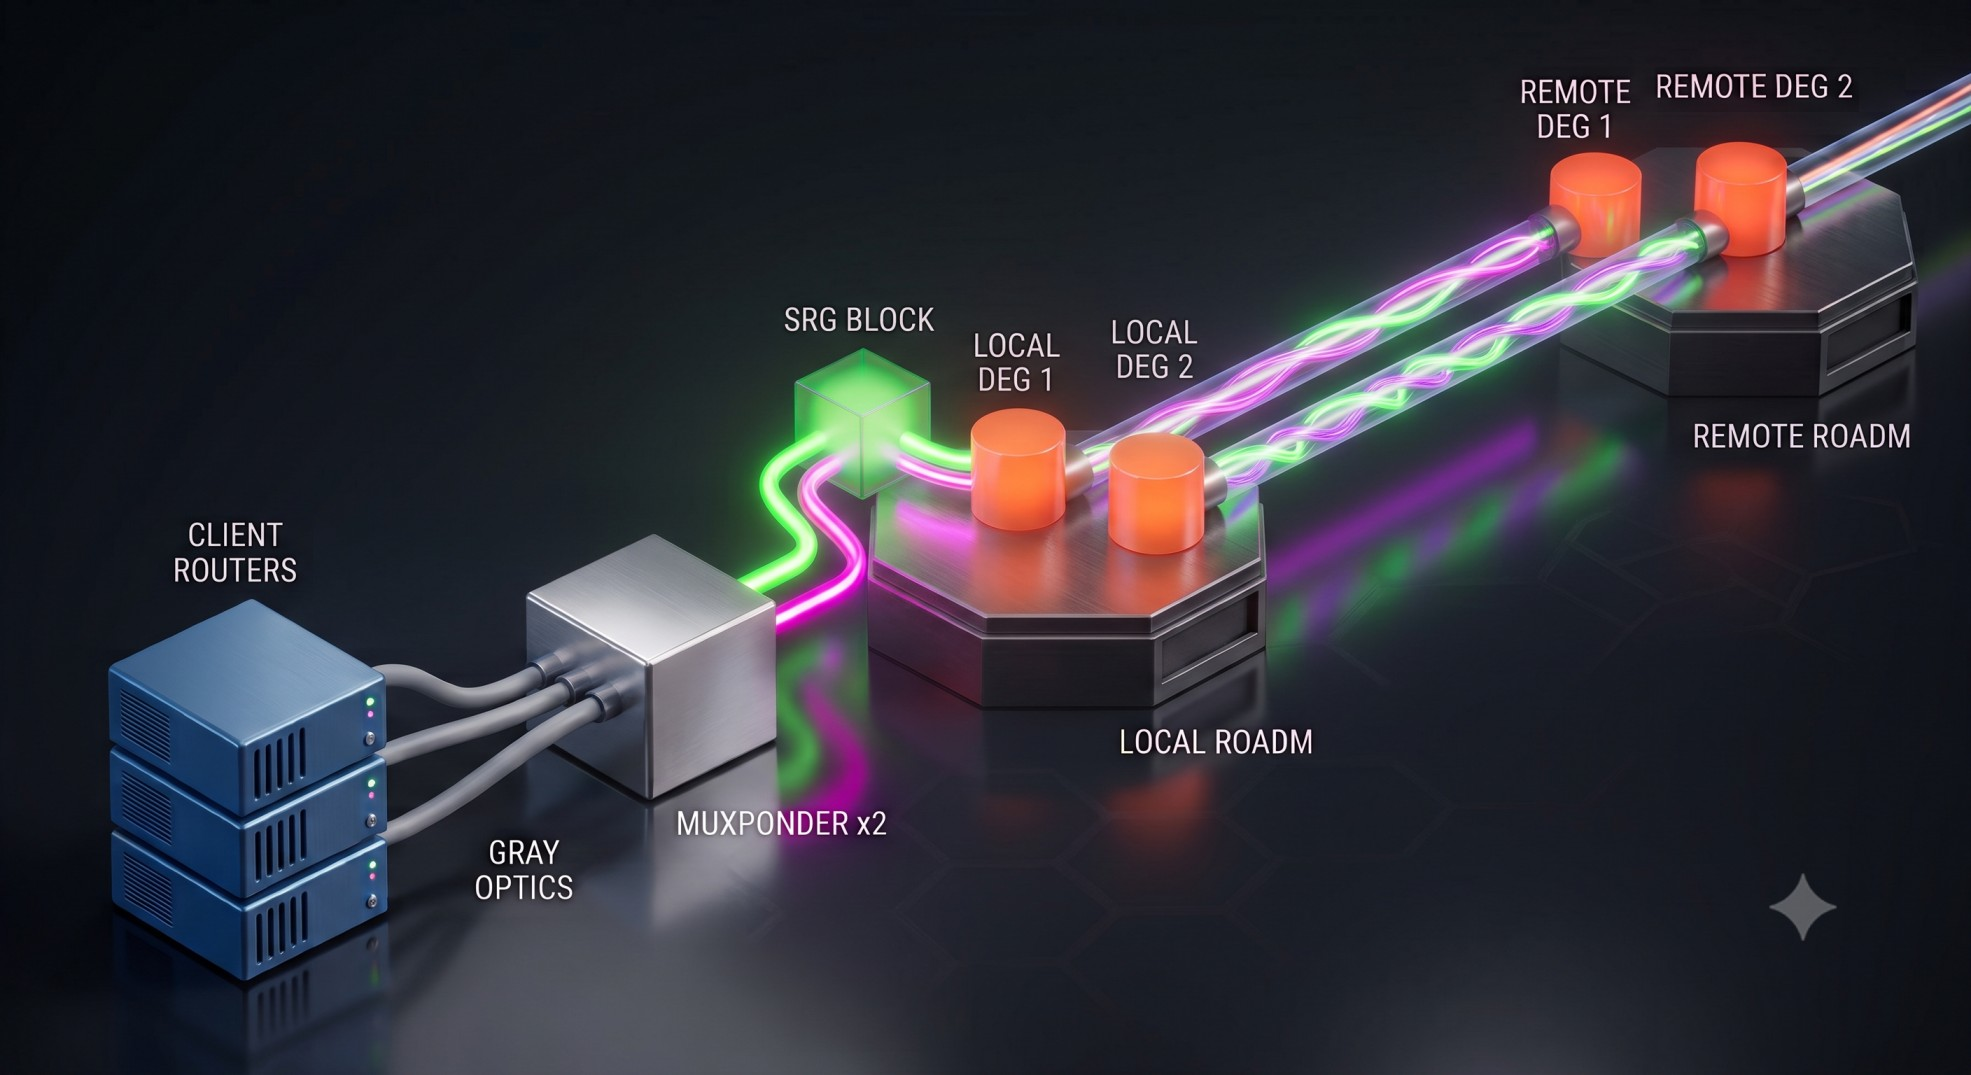
\includegraphics[width=0.8\textwidth]{Gemini_simple_optical_2_link_transmission.jpg}
    \caption{Optical Connectivity with Parallel Links}
    \label{fig:Gemini_simple_optical_2_link_transmission}
\end{figure}
When multiple connections are setup to a single SRG, they cannot transmit on the same frequency simultaneously. As we can see in Fig.~\ref{fig:Gemini_simple_optical_2_link_transmission}, connectivity through two different links from the muxponder to ROADM's SRG block requires two different wavelengths. Because the standard SRG multiplexes all local signals onto a shared internal path toward the DEGs, reusing identical frequencies here causes catastrophic optical interference. In contrast, different DEG blocks manage entirely separate physical fiber cables. Therefore, the same optical frequency can be freelys reused across different DEGs, because the light paths remain physically isolated from one another. Managing these complex wavelength rules and routing matrices requires robust centralized intelligence, as manual configuration of massive DWDM networks is practically impossible. To orchestrate this intricate physical hardware efficiently, the overall network architecture is fundamentally divided into distinct operational network planes.
\subsection{Network Planes}
Traditional network architectures are logically divided into three distinct operational planes. As depicted in the standard architectural model in Fig.~\ref{fig:network_planes}, these are the management plane, the control plane, and the data plane. The data plane encompasses the physical hardware components, and it is primarily responsible for forwarding the actual optical traffic. Above this physical layer, the control plane hosts the distributed routing intelligence. Control plane entities reside within each individual network node, and they communicate horizontally to discover network topology and establish data connections. Finally, the management plane provides a centralized oversight system, where human operators monitor network performance and configure long-term administrative policies.
\begin{figure}[htbp]
    \centering
    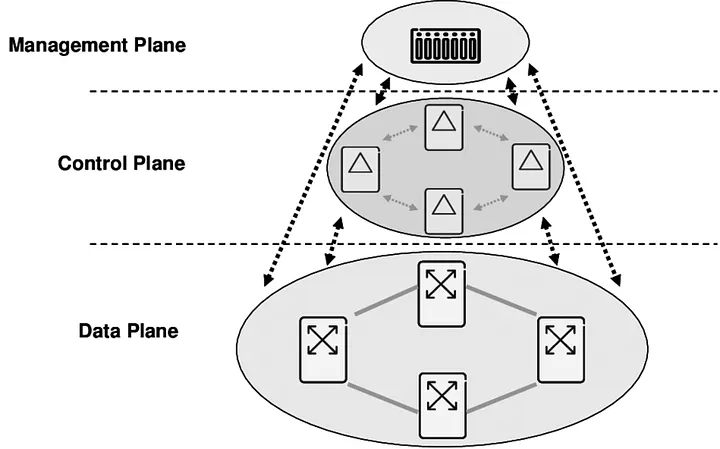
\includegraphics[width=0.8\textwidth]{network_planes.png}
    \caption{Network Planes}
    \label{fig:network_planes}
\end{figure}
To automate optical network operations, Generalized Multiprotocol Label Switching (GMPLS) was widely adopted within the distributed control plane~\cite{4814809}. GMPLS enables dynamic lightpath provisioning, and it allows individual nodes to automatically recover from sudden fiber failures. However, this distributed approach possesses significant operational limitations. Because each node calculates paths independently, the network struggles to achieve optimal, global resource allocation. Furthermore, GMPLS suffers from severe interoperability issues across different equipment manufacturers. Vendors frequently implement proprietary extensions to the standard routing protocols, and this inevitably creates strict vendor lock-in. Overcoming these fundamental limitations requires a unified, vendor-agnostic control architecture.
\subsection{Software Defined Network}
Software-Defined Networking (SDN) emerged to resolve the severe limitations of distributed control protocols. SDN fundamentally transforms network architecture, because it physically decouples the control plane from the underlying data forwarding plane. In an SDN architecture, routing intelligence is entirely consolidated into a centralized, software-based controller. This centralized model provides a comprehensive, real-time view of the entire network topology, and this allows the controller to perform highly complex path computations across the infrastructure.
\begin{figure}[htbp]
    \centering
    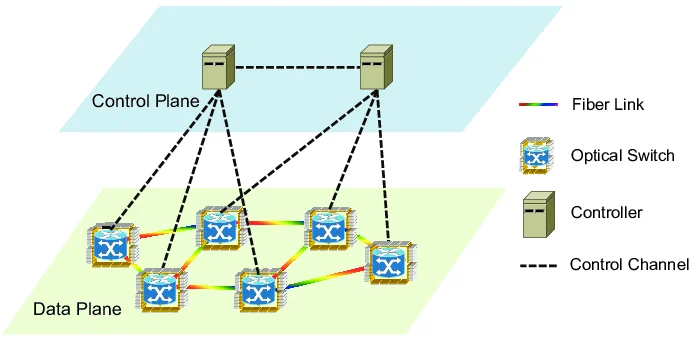
\includegraphics[width=0.8\textwidth]{sdon.png}
    \caption{Software Defined Optical Network~\cite{sdonOnos}}
    \label{fig:sdon}
\end{figure}
In packet-switched networks, the SDN controller typically manages electrical data flows utilizing the OpenFlow protocol. OpenFlow directs traffic through two distinct mechanisms: reactive and proactive forwarding. In reactive forwarding, an unknown data packet triggers a request to the controller, and the controller subsequently calculates and installs a new forwarding rule. Conversely, proactive forwarding pre-installs all necessary flow rules directly into the switch hardware, which completely eliminates the latency associated with remote controller queries. While OpenFlow efficiently manages electrical packet switching, complex optical transmission hardware requires highly structured configuration models. To address this, the telecommunications industry adopted the Yet Another Next Generation (YANG) data modeling language. YANG standardizes how physical device parameters are structured, and this eliminates the historical problem of vendor lock-in. Because all participating manufacturers conform to these standardized schemas, the SDN controller achieves a truly vendor-agnostic nature. This standardization provides massive interoperability benefits, as network operators can seamlessly integrate hardware from different suppliers within the same physical infrastructure.


Prominent industry frameworks, such as OpenConfig~\cite{openconfigYang} and OpenROAD~\cite{openroadmYang}, define these unified YANG models specifically for optical networks. These comprehensive models explicitly define critical hardware information, which includes physical port mappings and internal component capabilities. Furthermore, they accurately represent complex optical parameters, such as supported operational modes and continuously tunable frequency ranges. To actively manipulate these YANG-modeled parameters, the SDN controller utilizes the Network Configuration Protocol (NETCONF). NETCONF securely connects to the physical optical devices, and it retrieves their current operational state directly into the centralized controller. Consequently, the controller possesses accurate hardware configurations, and it uses this critical data to compute optimal end-to-end optical connections.

Managing optical transmission hardware requires complex configuration, and modern SDN controllers utilize structured workflows to provision these physical networks. As illustrated in Fig.~\ref{fig:sdon} architecture, the provisioning process begins when the controller receives a service connectivity request, which is typically formatted using the standard Transport API (T-API). To ensure signal viability, the controller gathers path data and physical impairment metrics, and it subsequently forwards this information to an external Quality of Transmission (QoT) estimation tool. This QoT tool communicates via RESTCONF or NETCONF, and it determines optimal device configurations such as modulation formats and required frequency slots. Following this estimation, the controller formulates a specific optical intent, and it passes these explicit instructions to the southbound device drivers. These drivers utilize the NETCONF protocol to configure the underlying transponders and ROADMs directly. Once the controller successfully orchestrates these physical hardware parameters, the infrastructure can finally establish the requested end-to-end optical connectivity.
\subsection{Optical Connectivity in SDN}
In Software-Defined Networking, an intent represents a high-level declarative policy. It defines what specific outcome the network should achieve, and it purposefully abstracts the low-level implementation details. Consequently, an optical intent specifies the exact desired characteristics of a physical lightpath. It outlines the necessary bandwidth and termination points, while it hides the underlying wavelength routing complexities from the user.
\begin{figure}[htbp]
    \centering
    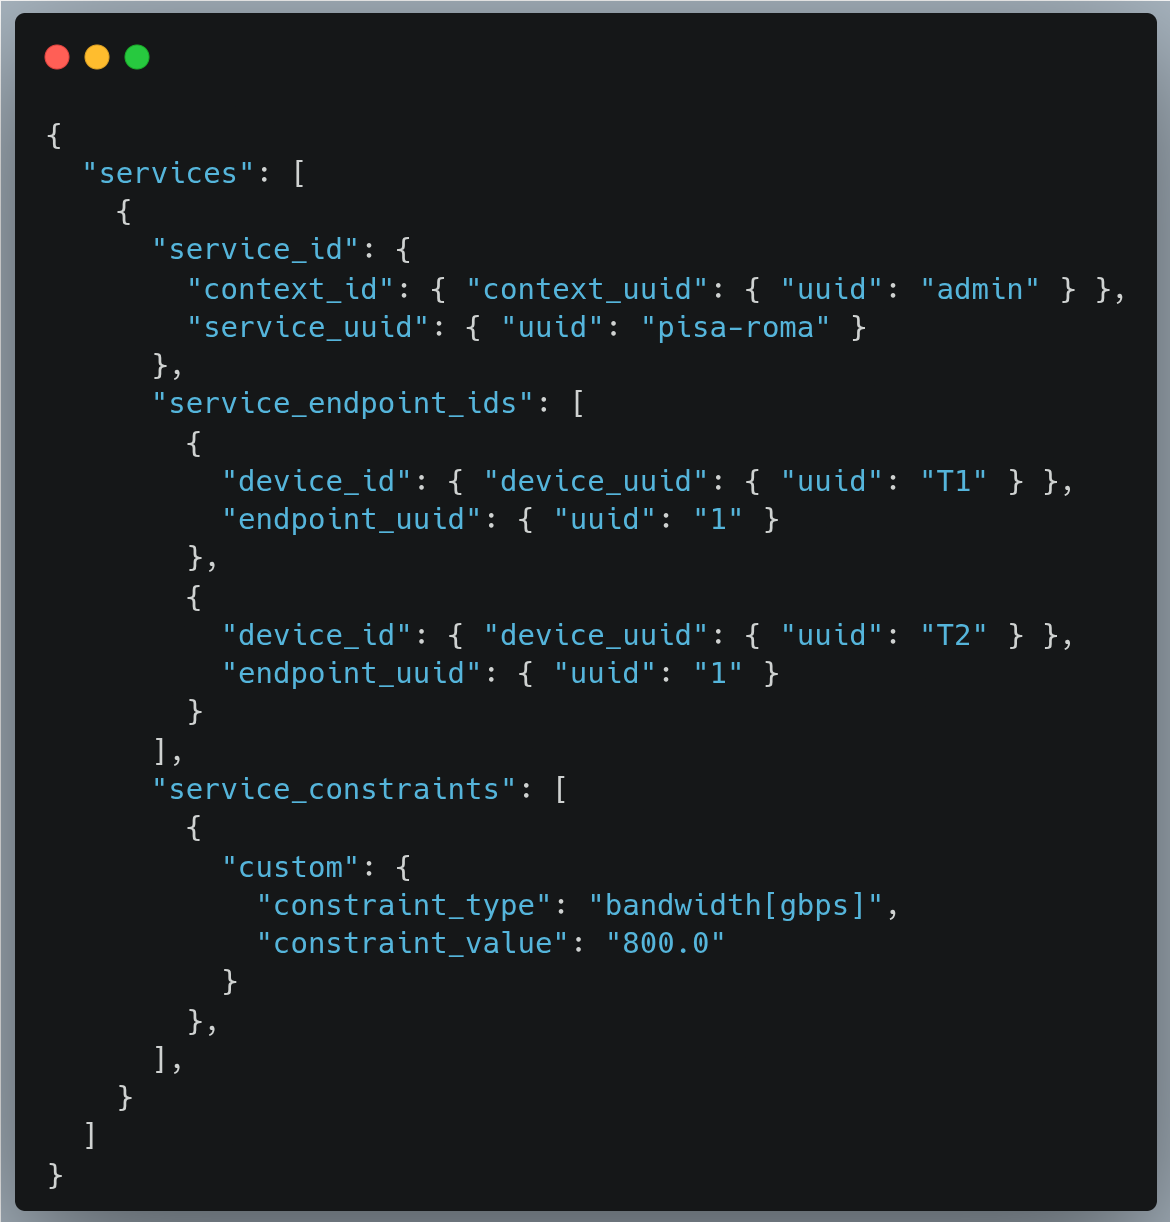
\includegraphics[width=0.8\textwidth]{optical_intent.png}
    \caption{An example optical connectivity intent in TeraFlowSDN}
    \label{fig:optical_intent}
\end{figure}
Network operators typically define these declarative intents using structured JavaScript Object Notation (JSON) files. The SDN controller ingests this formatted JSON payload, and it dynamically computes the optimal physical path to satisfy the given constraints. For example, a representative service configuration in Fig.~\ref{fig:optical_intent} defines a discrete optical intent between two distinct endpoints. The request dictates a unidirectional optical connection, and it links a source device labeled~\emph{T1} to a destination device labeled~\emph{T2}. Furthermore, this specific intent enforces a flex-grid network constraint, and it explicitly demands a massive transmission bitrate of~\emph{800.0 Gbps}. Once the controller parses this JSON request, it must translate the abstract intent into a physical optical transmission. This operational translation involves calculating a continuous physical path, assigning an appropriate optical spectrum, and actively configuring the underlying hardware devices. Because the SDN controller must simultaneously determine the optimal route and allocate contiguous frequency slots, the mathematical computation becomes highly complex. Within modern software-defined optical networks, this fundamental routing challenge is formally known as the Routing and Spectrum Assignment (RSA) problem~\cite{algorithmsRSATaxonomy}.
\section{Motivation}
Modern optical networks face significant operational challenges, and these include multi-node path routing and complex optical device interoperability. Furthermore, the transition to EONs demands highly dynamic resource allocation, which must be centrally managed by an SDN controller. Within this advanced software-defined environment, the RSA problem becomes critically important. The centralized SDN controller must continuously calculate viable lightpaths, and it must simultaneously allocate contiguous frequency slots across multiple optical nodes.

This routing complexity is severely amplified when multiple parallel fiber links exist between adjacent hardware nodes. Combining dense parallel links with granular flex-grid spectrum allocation creates massive combinatorial possibilities, and this ultimately leads to an exponential computational time complexity. Exact mathematical algorithms struggle to process these massive routing matrices in real-time, which necessitates the development of highly efficient heuristic approaches. A well-designed heuristic can rapidly evaluate potential optical routes, and it can perform spectrum assignment without overwhelming the centralized controller's processing capacity.

To explore these advanced path computation techniques, we can utilize modern open-source SDN platforms like  European Telecommunications Standards Institute~\emph{(ETSI) TeraFlowSDN (TFS)}~\cite{aboutTFS}. Integrating custom RSA heuristics within the TeraFlowSDN controller provides an optimal testing environment, and it allows for the practical evaluation of complex EON constraints. Ultimately, the massive computational burden of modern optical routing serves as the primary motivation for this research. Addressing these critical scaling challenges provides a clear scope for study, and it drives the need for optimized, SDN-based routing algorithms.

\section{Objectives and Contributions}
This thesis systematically addresses the challenges of RSA over parallel optical links. To achieve this, the research pursues several core objectives, and it delivers tangible technical contributions to the TFS ecosystem.
The primary research objectives focus on analyzing the fundamental constraints of modern optical networks, and they evaluate existing software-defined solutions. These core goals include:
\begin{itemize}
    \item \textbf{Analysis of Optical Standards and Controllers:} To investigate flexible-grid operational principles based on ITU-T G.694.1 standards, and to evaluate how industry-standard SDN controllers manage complex optical intents.
    \item \textbf{Review of RSA Algorithms:} To explore current algorithmic strategies for multi-hop optical networks, and to identify their computational inefficiencies when processing dense parallel links.
    \item \textbf{Examination of TFS Capabilities:} To analyze device discovery mechanisms within TFS, specifically focusing on the architectural constraints of the OpenConfig and OpenROADM device drivers.
\end{itemize}

Building upon these objectives, this research introduces an optimal RSA framework, and it integrates this solution directly into the TFS controller. The specific technical contributions are summarized as follows:
\begin{itemize}
    \item \textbf{Enhancement of Optical Device Drivers:} The existing TFS OpenConfig and OpenROADM drivers are significantly extended. This enhancement implements custom filters to extract vendor-agnostic parameters, which include operating frequencies, transport types, and power levels.
    \item \textbf{Design of an Optimized RSA Algorithm:} A novel RSA algorithm is formulated specifically for multi-fiber topologies. It utilizes the \emph{networkX}~\cite{networkX} library to model parallel edges, and it introduces a bitmap-based bitwise intersection method to rapidly compute contiguous spectrum availability.
    \item \textbf{Development of the POC Microservice:} A dedicated Path Optical Computation (POC) microservice is engineered and integrated into the TFS ecosystem. This execution engine autonomously calculates multi-hop lightpaths, and it effectively mitigates the NP-hard~\cite{wangRSAInfocom} computational bottlenecks associated with exponential routing permutations.
    \item \textbf{WebUI Integration:} The TFS Web User Interface is comprehensively upgraded to reflect complex physical and logical network states. This graphical update visualizes device endpoint capabilities, real-time spectrum slot availability, and dynamic RSA computation outputs.
\end{itemize}

By fulfilling these technical goals, this thesis delivers a comprehensive end-to-end solution. It successfully bridges low-level physical device configuration with high-level algorithmic path computation and graphical user interaction.

\section{Organization of the Thesis}
The remainder of this thesis is logically structured to guide the reader through the theoretical background, the proposed algorithmic solution, the system implementation, and the final evaluation. The document is organized as follows:
\begin{itemize}
    \item \textbf{Chapter 2:} Introduces the cloud-native TFS architecture, which efficiently manages these complex physical optical devices. Furthermore, the chapter thoroughly explains the RSA problem across multiple parallel fiber links. Finally, it reviews existing RSA algorithms, and it highlights their critical limitations within practical multi-fiber SDN environments.
    \item \textbf{Chapter 3:} Formally establishes the research problem and introduces the mathematical representation of the challenge. It details the graph modeling techniques used to represent topologies with parallel links. And then breaks down the proposed RSA algorithm, covering bandwidth computation, path discovery, bitmap-based slot calculation, and acquisition.
    \item \textbf{Chapter 4:} Dives into the software architecture of the proposed solution. It outlines the modifications made to TFS—including device driver enhancements, database schema extensions, and the RSA Computation Module. Furthermore, it details the development of the POC and the corresponding WebUI enhancements for spectrum visualization.
    \item \textbf{Chapter 5:} Outlines the experimental environment used to validate the proposed system. It describes the physical and virtual infrastructures, the configuration of emulated optical devices, the setup of network topologies, and the deployment procedure utilizing MicroK8s.
    \item \textbf{Chapter 6:} Represents a comprehensive analysis of the system's performance. It covers functional validation, computational performance, and spectrum utilization efficiency. The chapter also provides a throughput analysis, a comparative study against baseline approaches, and a statistical discussion of the simulation results.
    \item \textbf{Chapter 7:} Final chapter summarizes the primary contributions of the thesis, discusses the current limitations of the implemented system, and suggests potential directions for future research and development.
\end{itemize}

\chapter{Background and Literature Review}
This chapter explores the architecture of the ETSI TeraFlowSDN controller, and it examines how this centralized software manages physical optical devices. Furthermore, it provides a detailed analysis of the~\emph{RSA} problem within modern elastic optical networks. The review specifically investigates how multiple parallel fiber links exponentially increase the computational complexity of continuous spectrum allocation. Finally, it evaluates previous algorithmic research addressing this problem, and it highlights the scope of practical heuristic implementations within software-defined optical environments.

\section{TeraflowSDN}
\subsection{Architecture and Ecosystem}
As we can see in figure~\ref{fig:tfs_architecture} TFS is a state-of-the-art, open-source SDN controller developed under ETSI to radically advance the orchestration of beyond 5G and 6G networks. Designed as a secure, cloud-native platform, TFS employs a microservices-based architecture orchestrated within Kubernetes environments, enabling individual control components to operate autonomously and scale independently. This inherent modularity provides an ideal ecosystem for integrating custom logic. Furthermore, the architecture is explicitly engineered to seamlessly integrate with modern Network Function Virtualization (NFV) and Multi-access Edge Computing (MEC) frameworks, including ETSI OpenSourceMANO. By unifying network and cloud resource management, TFS equips telecom operators and hyperscale cloud providers with efficient automation, business agility, and dynamic service provisioning across complex, multi-tenant optical and packet transport infrastructures.
\begin{figure}[htbp]
    \centering
    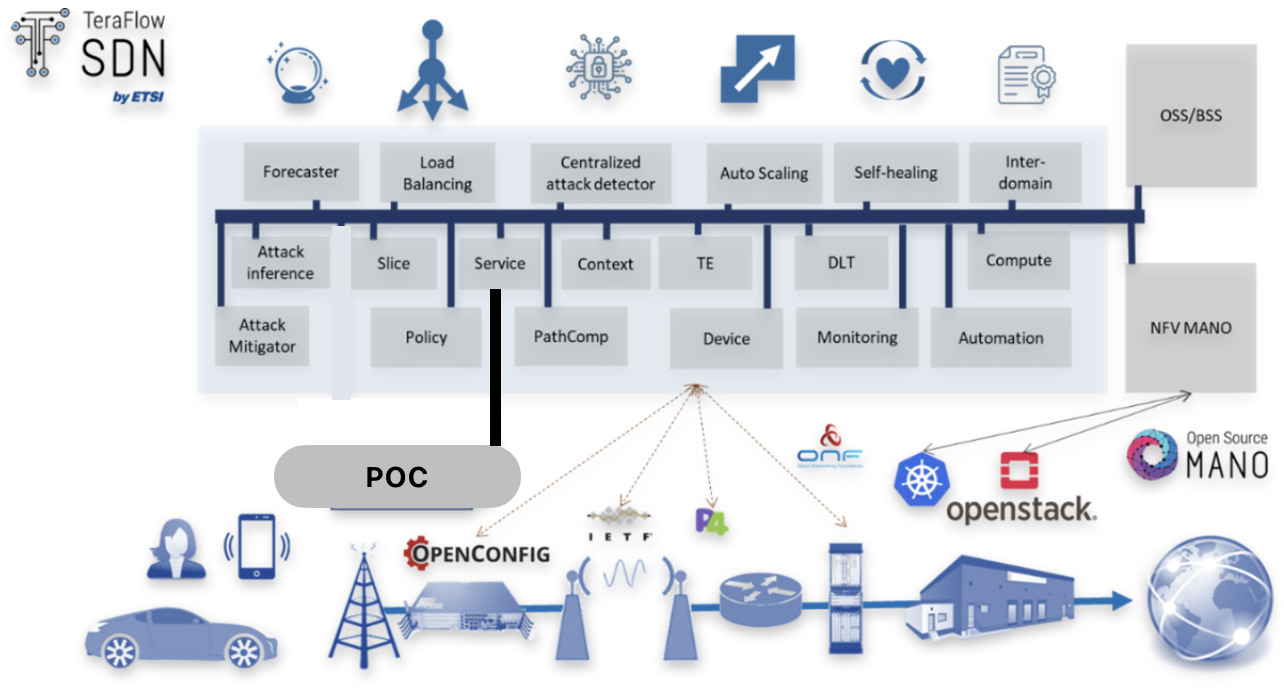
\includegraphics[width=0.8\textwidth]{tfs_architecture.png}
    \caption{TFS Architecture~\cite{tfsArchitecture}}
    \label{fig:tfs_architecture}
\end{figure}
\subsection{Core services}
The TFS ecosystem relies on a coordinated suite of specialized microservices. These services communicate via Remote Procedure Calls (gRPC), and they execute dynamic network configurations. At the core of this architecture operates the~\emph{ContextService}. It acts as the central database manager, and it maintains a definitive global view of all topologies, devices, and active network slices. The~\emph{DeviceService} directly manages all southbound interfaces. It utilizes a modular framework of vendor-agnostic drivers, and these drivers dynamically configure the underlying physical hardware.

Furthermore, the~\emph{ServiceService} functions as the primary service orchestrator. It receives provisioning requests from the network operator via the WebUI, and it subsequently forwards these requests to the corresponding provider. Network operators visually monitor all fundamental operations through this WebUI, which provides detailed topology and telemetry displays. Finally, several complementary microservices support the broader ecosystem. These auxiliary components execute policy-driven automation, and they ensure highly efficient network orchestration. These core components of TFS provide a complete environment to address the Routing and Spectrum Assignment problem. Services like the ServiceService, DeviceService, and ContextService provide a comprehensive framework, and they enable the advanced implementation of optical controllers. Consequently, this modular architecture allows the system to solve complex optical domain challenges, such as the RSA problem.
\section{Routing and Spectrum Assignment}
In modern EONs, resource allocation becomes an NP-hard computational challenge~\cite{rsaHeuristicSliced}. The ITU standards mandate precise flex-grid specifications, and this strict standardization inherently complicates resource management. To effectively solve this complex problem, the process is typically divided into two distinct phases. These two phases are the initial path routing and the subsequent spectrum assignment.

During the routing phase, the controller must identify valid physical paths across complex topologies. In large network architectures, computing these routes frequently utilizes~\emph{k-shortest} path algorithms. Because these expansive topologies offer numerous routing options, the path calculation requires extensive recursive computations. Furthermore, deploying multiple parallel links between adjacent nodes introduces another severe layer of complexity. When the controller evaluates these parallel physical fibers, the search time increases exponentially for a uniform number of links ($L^H$ in worst cases). Consequently, determining the optimal physical path becomes highly resource-intensive before any frequency spectrum is even considered.

Once a physical route is established, the controller must execute the spectrum assignment phase. This allocation must strictly adhere to ITU-T G.694.~\cite{itu694} standards, which govern all flex-grid operations. The standard anchors the entire DWDM spectrum to a reference central frequency of~\emph{193.1 THz}. And as we already discussed before, the standard establishes a nominal central frequency granularity of 6.25 GHz, and it enforces a minimum slot width granularity of 12.5 GHz. Using these indivisible building blocks, every valid spectrum assignment must fundamentally satisfy two primary physical constraints~\cite{algorithmsRSATaxonomy}.

First, the spectrum continuity constraint dictates that the exact same frequency index must remain identical across the entire path~\cite{algorithmResearchRSAONR}. In multi-fiber infrastructures, the optical signal may shift spatially between parallel fibers, provided no internal switching restrictions exist at the cross-connects~\cite{efficientDynamicRSAEon}. However, frequencies strictly cannot be reused on the shared add-drop side of the optical node. Second, the spectrum contiguity constraint requires that the assigned frequency slots must be strictly adjacent. These adjacent slots form a contiguous block, and this block precisely matches the variable bandwidth demands~\cite{algorithmsRSATaxonomy}.

These strict rules inevitably cause frequency fragmentation across the infrastructure. Because the controller must locate uniformly available contiguous blocks, this spectrum diversity introduces massive computational overhead. When this granular allocation constraint combines with the already exponential path selection phase, the overall RSA calculation becomes exceptionally difficult. Therefore, advanced RSA algorithms must evaluate the network state as a unified allocation matrix, and they must process both routing and spectrum constraints simultaneously to efficient transmission of optical signals. To address these massive computational challenges, researchers have proposed various algorithmic solutions. Consequently, the following section reviews this previous work, and it examines existing RSA implementations within software-defined environments.
\section{Previous Work}
\subsection{Algorithmic Approaches}
To solve the RSA problem, intense research has been dedicated to developing sophisticated RSA algorithms~\cite{distanceAdaptive}. Over time, these algorithms have evolved from basic wavelength assignment models into complex, multi-metric optimization strategies designed to maximize network throughput and accommodate diverse, dynamic traffic demands~\cite{algorithmsRSATaxonomy}. Early approaches sought to decouple the routing and assignment phases to mitigate computational bottlenecks. Foundational algorithms employed greedy heuristics and K-shortest paths to maximize single-hop traffic while strictly enforcing standard wavelength continuity~\cite{heuristicWSAMultihop}. As networks transitioned to flex-grid EONs, researchers introduced offline traffic sorting heuristics to groom them more efficiently. For instance, the Minimum Hops with Least Slots (MHLS) algorithm prioritizes connection requests by calculating a sorting parameter:
\[
    NP=Hops \times Slots
\]
By serving~\emph{smaller} requests first, the algorithm minimizes overall blocked traffic~\cite{rsaHeuristicSliced}. More dynamic approaches have integrated custom cost functions to balance multiple network metrics simultaneously. For example, the~\emph{FRSO-RSA} algorithm evaluates candidate alternative routes by actively steering traffic away from congested or unreliable paths using the following cost function:
\[
    cost_c = \alpha \times PF_c + (1 - \alpha) OU_c
\]
where $PF_c$ represents the physical failure rate of the path, $OU_c$ denotes the spectrum occupancy rate, and $\alpha$ acts as an adjustable weight parameter~\cite{failureProbability}.
To combat the specific issue of contiguity-induced fragmentation, recent literature has shifted toward~\emph{next-state-aware} algorithms. Metrics such as Maximum Spectrum Completeness (MSC) are used to evaluate how a current assignment will impact future capacity, actively selecting routes that preserve large, unbroken blocks of spectrum~\cite{maximumSpectrumCompleteness}. Other strategies introduce highly dynamic link-weighting mechanisms that actively draw traffic toward links harboring the largest unfragmented spectrum slices rather than just looking at total available capacity~\cite{spectrumStatusAware}. When fragmentation inevitably occurs during the network's lifecycle, complex defragmentation algorithms utilizing Integer Linear Programming (ILP) and Resource Dependency Digraphs (RDD) are deployed to mathematically recalculate and shift existing lightpaths without altering their physical routes~\cite{optimizingSpectrumAllocationEON}. Furthermore, advanced meta-heuristics like Genetic Algorithms and probabilistic models like Markov Decision Processes (MDP) have been explored to navigate massive solution spaces and predict network states~\cite{routingModulation,adaptiveRSAFlex}.
\subsection{Existing Implementations}
To address the NP-hard complexities of optical network management, theoretical research has developed sophisticated RSA algorithms designed to mitigate severe spectrum fragmentation and maximize throughput. These strategies have evolved from foundational, decoupled wavelength assignment models and offline traffic sorting heuristics, into dynamic, multi-metric optimization approaches that actively steer traffic away from congested or unreliable paths. Recent literature also heavily emphasizes~\emph{next-state-aware} metrics, dynamic link-weighting, and complex defragmentation models. However, extensive taxonomic reviews reveal a prevailing structural limitation: the vast majority of these theoretical solutions are designed exclusively for one-dimensional, single-fiber-per-link topologies. When applied to multi-fiber scenarios, these models must treat parallel links either as physically invalid aggregated bandwidth or as entirely separate logical links, inevitably triggering a state-space explosion and unmanageable computational complexity.

In practical deployments, industry-standard SDN controllers like ONOS~\cite{odtnONOS} and OpenDaylight (ODL)~\cite{odlTPCE} attempt to manage these topologies using robust, graph-based routing engines, yet they fundamentally struggle with the same spatial constraints. In both controllers, optical connections are treated as strictly matched port-to-port links; thus, multiple parallel fibers between the same devices are mapped as entirely distinct and independent topological edges. When computing routes via standard K-Shortest Path algorithms, the topology engine outputs every permutation of these parallel links as a completely independent path sequence. Consequently, the subsequent spectrum allocation phase applies strict isolation, evaluating spectrum continuity and contiguity sequentially on a strict per-path basis. If an allocation attempt experiences wavelength contention on one parallel link, the controller discards the effort and must iteratively re-run the entire RSA verification from scratch on the next topological path permutation. In complex, highly meshed topologies featuring multiple parallel links, this exhaustive, sequential path-by-path iteration causes exponential computational overhead, often leading to unacceptable latency and dynamic provisioning timeouts. These systemic shortcomings in both theoretical models and practical SDN implementations highlight a critical research gap, presenting the opportunity to design a dynamic, spatially-aware optical controller within the TFS ecosystem that evaluates parallel ports concurrently to bypass sequential iteration and enable highly scalable lightpath establishment.

\chapter{Problem Definition and Proposed Solution}
Previous chapters highlighted the computational challenges of RSA in networks featuring parallel links. This chapter formally addresses that problem by presenting a structured, algorithmic approach. First, it logically represents the physical network infrastructure through graph-based topological modeling. Next, it explores multiple strategies to perform efficient path computation across these complex topologies. Following this, it investigates the spectrum assignment operation to allocate resources along the discovered routes. By evaluating these various schemes, this chapter ultimately formulates and adopts an optimal, integrated solution for the parallel-link RSA challenge.


\section{Problem Statement}
While previous chapters established the theoretical complexities of EONs, implementing a practical solution requires overcoming specific architectural bottlenecks. First, the SDN controller must dynamically extract vendor-agnostic hardware capabilities, and it must independently determine appropriate transmission modulation formats. Without this automated physical awareness, the controller cannot accurately provision viable optical connections.

Furthermore, the core algorithmic challenge lies in resolving the Routing and Spectrum Assignment problem across complex multi-fiber topologies. Because parallel links introduce massive combinatorial possibilities, computing an optimal path while enforcing spectrum contiguity often causes exponential computational delays. Therefore, the system strictly requires a highly efficient mathematical mechanism to maximize spectral capacity, and this mechanism must actively prevent unnecessary frequency fragmentation.

Finally, these complex internal routing decisions must be effectively visualized for network operators. The system must provide a comprehensive graphical interface, which clearly displays dynamic spectrum availability and physical routing paths. To resolve these interconnected challenges simultaneously, this thesis introduces a comprehensive software-defined solution. The foundational logic of this solution is detailed in the following section, which formally presents the proposed RSA algorithm.


\section{Proposed Algorithm}
In this section we are going to disucss the fundamental logic of the proposed Routing and Spectrum Assignment algorithm. To execute efficient path routing, the methodology utilizes an advanced graph abstraction model. Furthermore, it incorporates a simple mathematical mechanism, and this mechanism dynamically calculates the required bandwidth and Frequency Slot Units (FSUs). To resolve strict spectrum contiguity constraints rapidly, the system implements a novel bitmap-based spectrum allocation technique. Finally, the section concludes with a comprehensive computational complexity analysis. This mathematical evaluation specifically assesses the path computation phase, and it determines whether the algorithm successfully achieves expected time complexity within parallel link configurations.
\subsection{Graph Modelling and Path Computation}
To achieve computationally efficient routing, the algorithm utilizes the NetworkX~\cite{networkX} library for complex network analysis. The algorithm converts the initial multi-graph instance~\emph{G} into a simplified graph abstraction, $G_{s}$, in which parallel physical links between nodes are collapsed into a single logical edge.
\begin{figure}[htbp]
    \centering
    \includegraphics[width=0.8\textwidth]{topo\_parallel\_link.png}
    \caption{Simple topology with non-uniform parallel links ($G$)}
    \label{fig:topo_parallel_link}
\end{figure}
As we can see in Fig.~\ref{fig:topo_parallel_link}, the topology is configured with 2 parallel links between~\emph{TP1 \& RDM1}, 2 parallel links between~\emph{RDM3 \& RDM4}, and 2 parallel links between~\emph{RDM5 \& TP2}. After the graph abstraction and simplification phase, the reforms as shown in Fig.~\ref{fig:topo_single_link}
\begin{figure}[htbp]
    \centering
    \includegraphics[width=0.8\textwidth]{topo\_single\_link.png}
    \caption{Simple topology with no parallel links ($G_s$)}
    \label{fig:topo_single_link}
\end{figure}
First, the algorithm constructs a multi-directed graph $G$ containing all parallel physical links. It then simplifies this topology into a separate graph $G_s$, which contains only single links between adjacent nodes. This structural simplification directly reduces the search complexity from an exponential scale to a linear scale. Simultaneously, the system generates an in-memory lookup table from the original graph $G$. This specialized table effectively bypasses full graph traversals, and it significantly accelerates future topological queries.

By routing over $G_s$ instead of the raw multi-graph, the controller completely prevents state-space explosion and computation latency. The algorithm utilizes Dijkstra's Shortest Path (DSP) to identify the primary shortest path, which is denoted as $dsp$. Furthermore, it computes additional candidate paths that satisfy the strict hop-count constraint $\mathcal{H} \leq \mathcal{H}_{min} + \Delta\mathcal{H}$. In this formula, $\mathcal{H}_{min}$ represents the absolute shortest path length, and $\Delta\mathcal{H}$ defines the allowed additional hops.
\begin{figure}[htbp]
    \centering
    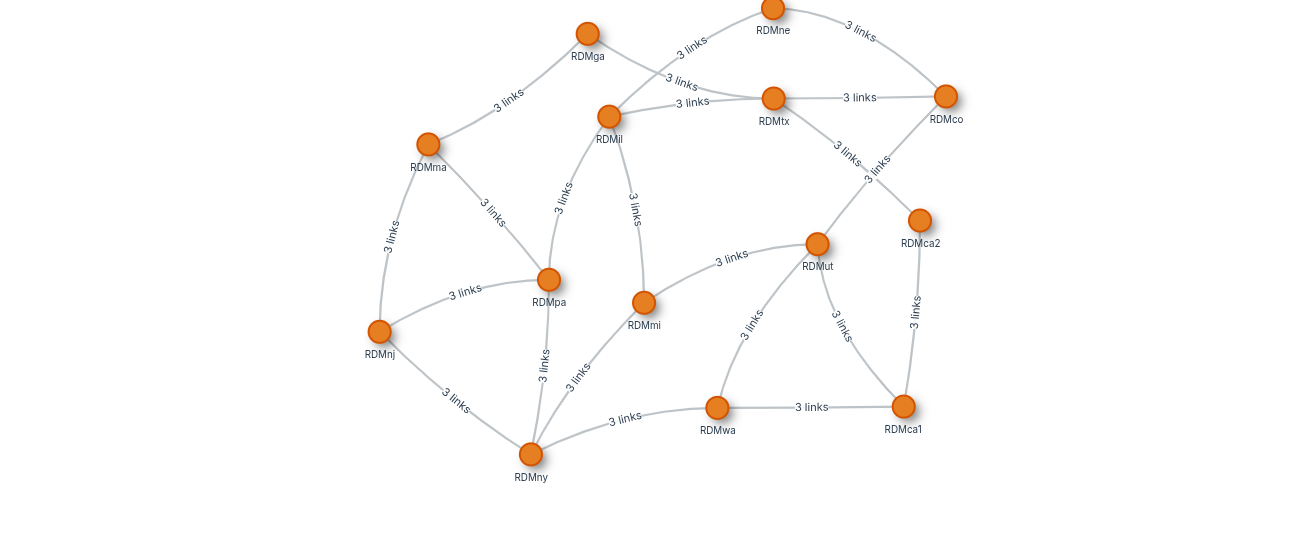
\includegraphics[width=1\textwidth]{parallel_graph_topo.png}
    \caption{Topological Graph Abstraction with NetworkX ($G_s$)}
    \label{fig:parallel_graph_topo}
\end{figure}
To select the optimal trajectory from these k-shortest candidate routes, the industry typically relies on baseline selection schemes. These standard schemes include Shortest Path First-Fit (SPFF) and Shortest Path Random-Fit (SPRF). Alongside these standard approaches, this thesis introduces a novel evaluation scheme called Shortest Path Spectrum Check (SPSC). The definitive selection among these schemes requires rigorous algorithmic analysis, and the final implemented choice is concluded later within the performance simulation chapter.

Once the optimal node trajectory is selected, it is formally designated as the $path\_node$. This $path\_node$ is subsequently mapped back onto the original multi-directed graph $G$ to facilitate parallel path expansion. During this specific expansion phase, the algorithm queries the pre-generated lookup table instead of traversing the entire multi-graph again. This highly efficient lookup identifies all possible parallel link combinations for the selected sequence of nodes. Following this parallel expansion, the system applies a similar path selection scheme to determine the final, exact physical path. Once this definitive physical path is established, the controller immediately forwards the connection request to the spectrum assignment phase. During this final phase, the system performs a specialized bitmap-based intersection across the selected links, and this mathematical operation locates the continuous and contiguous frequency slots required for transmission.

\subsection{Bandwidth and FSU Computation}
Following the path selection, the proposed algorithm determines the required spectral bandwidth ($B_r$) for the requested optical service. Upon receiving a connection request, the controller extracts the target transmission bitrate ($R_b$), expressed in Gigabits per second (Gbps), directly from the submitted TFS service descriptor. The required bandwidth is then mathematically derived using the following formulation:
\[
    B_r = \frac{R_b}{n}(1 + \alpha)
\]
where $n=log_2M$, and M represents the utilized modulation format. While several factors influence the required bandwidth calculation~\cite{ntiaBandwidth}, this standard formula simplifies the process for the controller.

Once $B_r$ is established, the controller computes the discrete number of FSUs ($N_r$) needed to accommodate the lightpath. In accordance with ITU-T flexible grid standards, the 12.5 GHz parameter is used to determine the total number of required FSUs. Concurrently, the finer 6.25 GHz granularity is used exclusively to define the central frequency of the allocation. The required number of slots is calculated as follows:
\[
    N_r = \frac{B_r}{12.5}
\]
\subsection{Bitmap-Based Spectrum Allocation}
During configuration, the device driver maps the operating frequencies of each endpoint into a bitmap, where each bit represents a~\emph{12.5 GHz} FSU. However, different hardware components support diverse spectrum ranges, such as C-BAND fractions versus full multi-band support.
\begin{figure}[htbp]
    \centering
    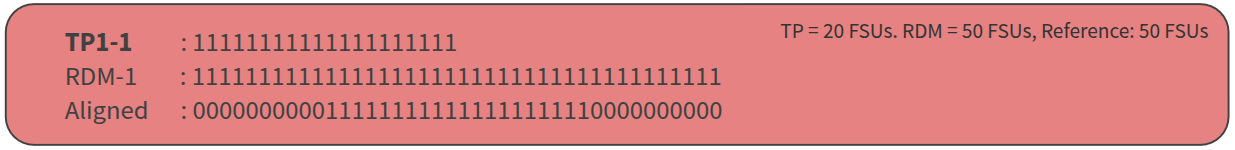
\includegraphics[width=0.8\textwidth]{spectrum_alignment.png}
    \caption{Spectrum alignment between heterogeneous FSU capacity}
    \label{fig:spectrum_alignment}
\end{figure}
In Fig.~\ref{fig:spectrum_alignment} we can see, the TP has 20 FSUs and the RDM 50 FSUs. To perofrm the bitmap-based execution, all device endpoints' FSU capacity should be aligned with the maximum range. Failing to account for these heterogeneous ranges causes inaccurate central frequency mapping, and this leads to potential signal collisions. To ensure absolute spectral continuity, the algorithm aligns all local bitmaps along the path to a standardized reference bitmap.

The algorithm then traverses the entire path to identify the maximum frequency range, and it determines the corresponding FSU capacity ($N_h$). It aligns each endpoint's capacity ($N_s$) to ensure bitwise spectral continuity across links with heterogeneous ranges, as shown in Fig.~\ref{fig:spectrum_alignment}. While investigating the links across the path, the system also identifies the add-drop links to ensure there is no frequency overlapping. It expands these add-drop parallel links to their own bitmaps, and it performs a bitwise intersection to determine the final available FSUs.
\begin{figure}[htbp]
    \centering
    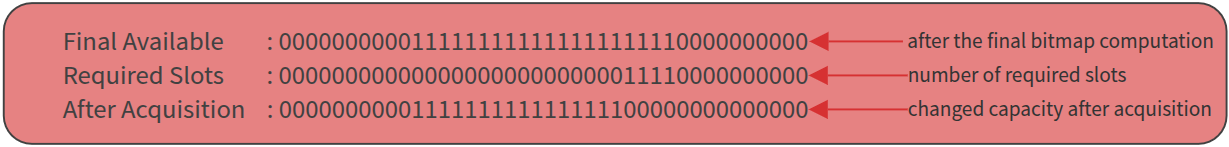
\includegraphics[width=0.8\textwidth]{spectrum_assignment.png}
    \caption{Spectrum Assignment Phase}
    \label{fig:spectrum_assignment}
\end{figure}
This resulting final bitmap represents the available spectrum, where~\emph{0} labels denote utilized slots and~\emph{1} labels denote available ones. According to Fig.~\ref{fig:spectrum_assignment} the algorithm performs a first-fit scan from the least significant bit, and it locates the first available FSU. It then checks for $N_r$ contiguous slots across the path. Because the previous hop-by-hop intersection already masked all used spectrum, finding these $N_r$ consecutive slots automatically guarantees both spectrum continuity and contiguity. If $N_r$ slots are contiguous across the entire path, the lightpath is provisioned; otherwise, the request is declined.
The complete algorithm is presented as follows:
\vspace{0.2cm}
\hrule
\vspace{0.1cm}
\noindent\textbf{Algorithm 1} RSA with parallel links
\vspace{0.1cm}
\hrule
\vspace{0.2cm}

\begin{algorithmic}[1] % [1] adds line numbers
    \REQUIRE Graph $G=(V, E)$, Links $\mathcal{L}$, Lightpath Request $\mathcal{R}$, Shortest Path Length $\mathcal{H}$ in hops, Allowed Additional Hops $\Delta\mathcal{H}$, Path selection scheme $\mathcal{PS}$, Spectrum selection scheme $\mathcal{SS}$.

    \STATE \textbf{Step 1:} Create graph $G$
    \FORALL{$link \in \mathcal{L}$}
    \STATE add devices as $V$, links as $E$ in $G$
    \ENDFOR
    \STATE Cache the Graph for future re-use
    \STATE \textbf{Step 2:} Path computation
    \STATE convert $G$ into $G_{s}$
    \STATE $dsp\leftarrow find\_path(G_{s}, \mathcal{PS}$)
        \STATE $dsp\leftarrow expand\_parallels(dsp, G, \mathcal{PS}$)
    \STATE $(dsp+\Delta\mathcal{H}) \leftarrow find\_path(G_{s}, \mathcal{H}, \Delta\mathcal{H}, \mathcal{PS}$)
        \STATE $(dsp+\Delta\mathcal{H})\leftarrow expand\_parallels(dsp+\Delta\mathcal{H}, G, \mathcal{PS}$)
    \STATE $path\_node \leftarrow dsp\ ||\ (dsp+\Delta\mathcal{H})$
    \STATE \textbf{Step 3:} Perform SA
    \STATE $B_r \leftarrow calculate\_bandwidth(bitrate, modulation)$
    \STATE $N_r \leftarrow required\_slots(B_r)$
    \FORALL{$hop \in path\_node$}
    \STATE get link information
    \STATE find $min, max$ frequencies
    \ENDFOR
    \STATE $N_h\leftarrow reference\_bitmap(max, min)$
    \FORALL{$hop \in path\_node$}
    \STATE get source, destination endpoint bitmaps
    \STATE align them with $N_h$
    \STATE perform intersection \& update $N_h$
    \ENDFOR
    \STATE apply $\mathcal{SS}$ on final $N_h$
    \STATE $\mathcal{R}$ is \textbf{success} or \textbf{blocked}
\end{algorithmic}
\vspace{0.2cm}
\hrule
\section{Complexity Analysis} \label{complexity_analysis}
The computational efficiency of the proposed~\emph{POC} is fundamentally anchored in its ability to decouple topological routing from spatial spectrum allocation. The initialization phase, which constructs the abstracted multi-graph $G$ with $V$ nodes and $E$ edges-has a linear space complexity of $\mathcal{O}(|V|+|E|)$. Let us assume we have $P$ parallel edges within $E$, the space complexity of $G_s$ stands for $\mathcal{O}(|V|+|E-P|)$. If we denote $L=E-P$, as the number of edges without parallels-the time required to compute $K$ shortest paths is $\mathcal{O}(KV(L+V\log V))$. Because redundant connections are abstracted into the simple graph $G_s$, an increasing number of parallel links $P$, does not impact the worst-case time complexity of the routing phase. To verify the time complexity, performance tests are conducted on well-known network references such as Pan-European (PANEU) and NSFNet models. A comprehensive empirical evaluation of these tests, including computational performance and statistical analysis, is detailed in the upcoming chapters.

\chapter{System Design and Implementation}
This chapter bridges the theoretical algorithm established previously with their practical software implementation. Specifically, it details the architecture engineered to natively support multi-fiber parallel links. First, we examine the structural enhancements integrated into the TFS ecosystem. Next, we outline the development of the RSA computational modules. Finally, the chapter details the operational deployment of the POC microservice.
\section{Contribution to Existing TFS Services}
This thesis significantly enhances the DeviceService microservice, and it introduces robust information extraction mechanisms for physical hardware. These targeted software improvements specifically optimize the OpenConfig and OpenROADM drivers, which ensures the accurate parsing of complex vendor-agnostic parameters. Furthermore, the WebUIService is comprehensively upgraded, and it now provides advanced graphical visualization capabilities for network administrators. This frontend enhancement allows operators to seamlessly monitor internal device configurations, and it clearly displays real-time spectrum availability alongside complex optical connectivity details.
\subsection{Enhancement of the DeviceService}
EONs are inherently heterogeneous, and they rely on equipment from various manufacturers. The industry utilizes standard YANG data models for device configuration. However, the expansive scope of YANG allows vendors to adopt significantly different internal data structures. Consequently, a monolithic data extraction technique is not always reliable. It frequently fails to capture the granular optical parameters, which are strictly required for advanced RSA computations.

To overcome this interoperability challenge, a dynamically adaptable extraction technique was integrated directly into the \emph{DeviceService}. This integration makes the software drivers significantly more robust, and it ensures highly efficient information extraction. The enhanced service rejects uniform parsing rules, and it instead utilizes specific \emph{device-model} based filters. The system dynamically identifies the exact hardware model, and it immediately applies a customized extraction profile. Furthermore, a default fallback filter is strictly enforced whenever an uncharacterized device is encountered.

Following this initial extraction, the driver logic executes a rigorous normalization phase. Critical operational data is systematically parsed, and it is subsequently synchronized with the central database. This phase captures essential physical endpoint indexes, transport types, and operational modes. Most importantly, it explicitly extracts the exact minimum and maximum frequency ranges for every device endpoint. This specific frequency data is absolutely critical for the spectrum assignment phase, because the algorithm must align the Frequency Slot Units into a standardized maximum range. Finally, several custom modifications were made within the device XML configurations, and these intentional variations rigorously validated this adaptable extraction methodology.
\subsection{Enhancement of the WebUI}
The WebUIService was significantly upgraded, and it now provides advanced device demonstration capabilities for network administrators. The updated graphical interface visualizes detailed capacity metrics, and it directly compares the two corresponding endpoints of any physical link. Furthermore, the dashboard implements precise frequency mapping, which strictly adheres to current ITU standards. Operators can easily monitor the dynamic spectrum state, because the interface clearly visualizes both used and available frequency slot units. Finally, the enhanced system details comprehensive optical connectivity information, and this allows users to efficiently track established multi-hop lightpaths.
\section{Parallel Optical Controller Microservice}
The ParallelOpticalController (POC) operates as a dedicated modular microservice, and it functions independently from the primary core services within the TeraFlowSDN ecosystem. To effectively manage complex optical environments, this specialized component interacts directly with the ContextService, DeviceService, and ServiceService. Through this coordinated internal communication, the POC successfully processes end-to-end optical connectivity requests.
\begin{figure}[htbp]
    \centering
    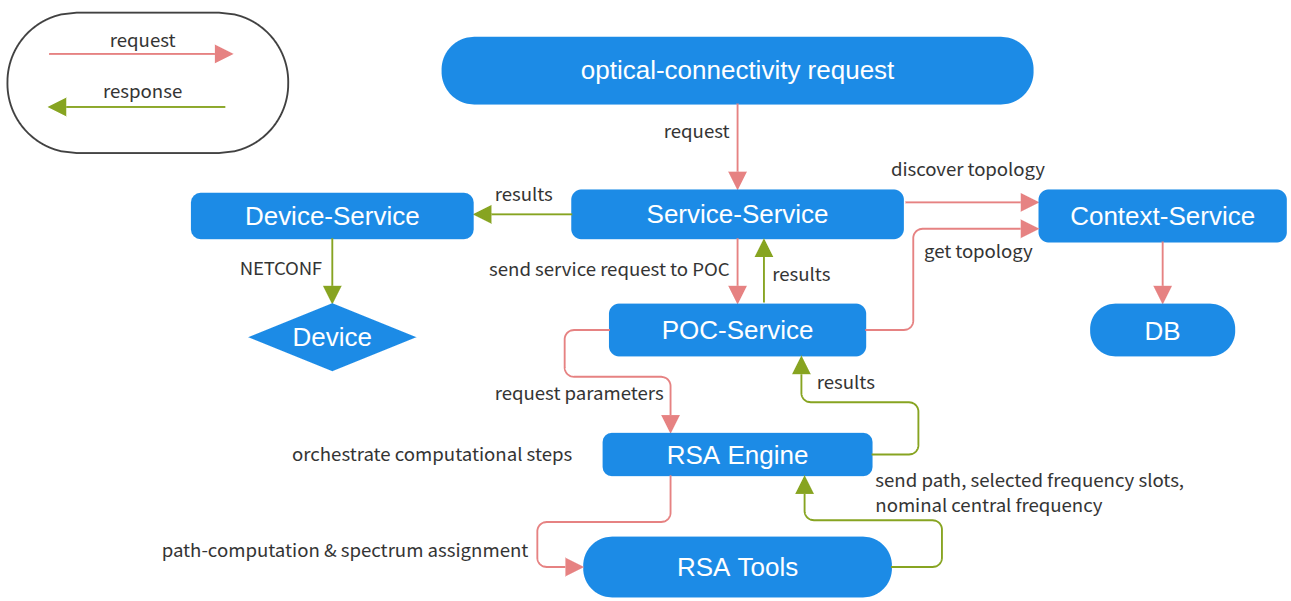
\includegraphics[width=0.8\textwidth]{poc_service_orch_3.png}
    \caption{Service Architecture of POC}
    \label{fig:poc_service_orchestration}
\end{figure}
As in Fig.~\ref{fig:poc_service_orchestration} when a network operator submits a new lightpath request, the execution logic within the POC follows a rigorous, three-phase computational pipeline. First, the system executes a simplified graph abstraction. This initial phase dynamically reduces the complex multi-fiber topology, and it effectively creates a highly manageable linear network model. Following this structural abstraction, the algorithm performs optimal path selection. This routing phase evaluates multiple candidate trajectories, and it precisely identifies the most efficient physical route. Finally, the controller executes the comprehensive spectrum assignment phase. During this critical final step, the system allocates continuous and contiguous frequency slots across the selected multi-hop architecture.

\subsection{Intra Service Communication}
The computational intelligence of the controller is systematically distributed across a suite of specialized Python submodules, and this complete execution workflow is visually summarized in Fig.~\ref{fig:poc_service_orchestration}. To maintain strict modularity, these internal helper functions are categorized into shared and core domains. The shared domain includes the \emph{ITUStandards.py} and \emph{RSATools.py} modules. The \emph{ITUStandards.py} module encapsulates the comprehensive ITU-T specifications for flexible-grid communications. During the initial device discovery phase, the hardware drivers utilize this specific module. They actively map the extracted transceiver types to their corresponding operating bands and frequency ranges.

Using this standardized frequency data, the \emph{RSATools.py} module generates a precise spectrum bitmap. This initial bitmap is immediately returned to the \emph{DeviceService}, and it is subsequently stored by the \emph{ContextService}. Furthermore, the \emph{RSATools.py} module executes the fundamental spatial operations of the controller. These mathematical tasks include complex graph generation, algorithmic path computation, and foundational spectrum assignment. Finally, both of these shared modules are integrated directly into the WebUIService, and they accurately render comprehensive visual representations of the optical configurations.

The \emph{RSA.py} module functions as the primary execution engine within the core domain. When the system processes a new lightpath request, it extracts the target parameters and delegates execution directly to this core module. Initially, the \emph{RSA.py} module calculates the necessary bandwidth and frequency slots based on the target bitrate. It then utilizes the shared spatial operations to orchestrate a rigorous hop-by-hop bitwise intersection. This intersection aligns the reference bitmaps, and it successfully identifies contiguous spectrum slots across the entire multi-fiber path. Once the spectrum is acquired, the algorithm removes the bitmap alignment, and it reformats the spectrum data into a standard integer. The final configuration is stored via the context-client, and the module returns a definitive provisioning response to the higher-level orchestration layer.

\chapter{Deployment and Testbed Setup}
This chapter outlines the physical and logical infrastructure utilized to evaluate the proposed algorithm of~\emph{POC}. It details the installation of the controller, the configuration of the network emulation environment, and the specific architectural constraints observed to maintain a stable testing environment.

\section{Deployment of TeraFlowSDN} \label{deployPOC}
The deployment of the controller begins by acquiring the TFS source code from the official repository~\cite{aboutTFS} and executing the standard setup procedure. However, to optimize server performance during the development and testing of the POC, a lightweight deployment strategy is recommended. TFS ecosystem contains auxiliary components that are highly resource-intensive. The most notable example is the centralized monitoring subsystem. Disabling these specific components mentioned in the official deployment documentation significantly reduces overall system overhead.

Beyond resource allocation, establishing a stable testbed requires strict adherence to several critical architectural and operational constraints:
\begin{itemize}
    \item Due to known networking conflicts between MicroK8s and Docker environments operating on the same host kernel, a distributed architecture was adopted. The primary server,~\emph{MASCARA}, is dedicated exclusively to the MicroK8s-based TFS deployment. Meanwhile, a secondary, independent server,~\emph{MONSTER}\footnote{MASCARA and MONSTER are located at DII, UniPi. Access is restricted and requires proper authorization.}, is utilized strictly to host the emulated network devices.
    \item To avoid interfering with the secondary server's default network interfaces, a dedicated Docker bridge network was provisioned exclusively for the device emulation environment. Once the deployment is initialized, static IP routes are configured between the hosts. This ensures seamless cross-server communication and grants the primary controller authorized access to the emulated devices.
\end{itemize}

\section{Deployment of POC}
As the official integration of the POC is currently ongoing, deployment relies on a supplementary repository~\cite{pocgit}. This repository must be cloned directly into the:~\emph{controller/src/} directory of the primary TFS ecosystem. Once positioned, the environment is initialized by executing the~\emph{deploy-parallel-optical-controller.sh} script. As outlined in Fig.~\ref{fig:poc_deploy}, this script automates the Docker image compilation, applies the Kubernetes manifests, and restarts the necessary auxiliary services to register the new controller:
\begin{figure}[htbp]
    \centering
    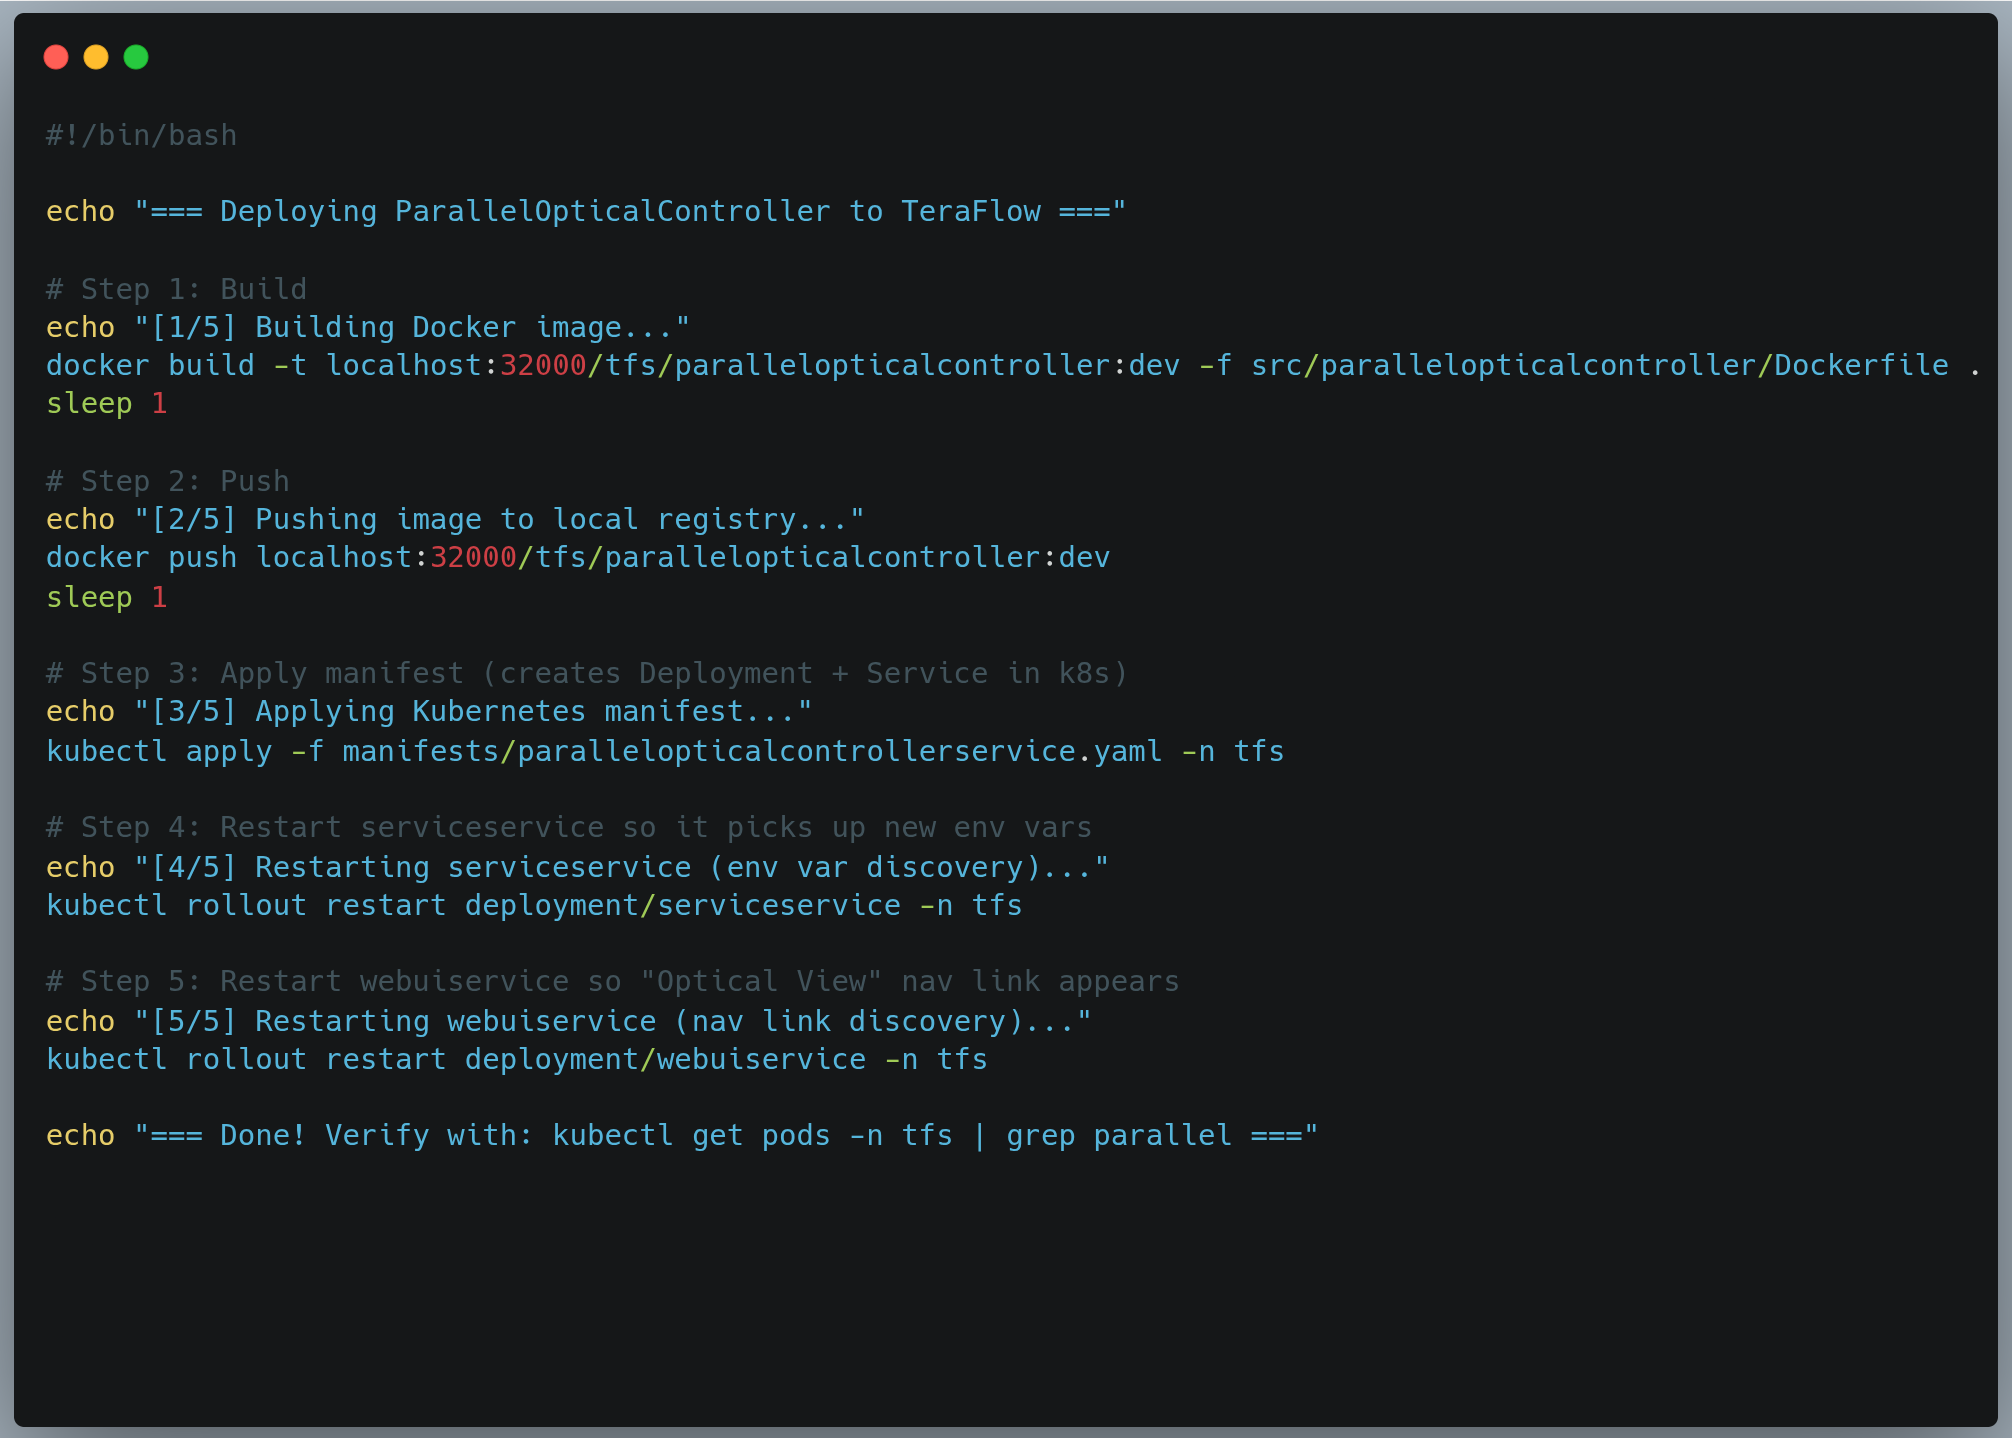
\includegraphics[width=0.8\textwidth]{poc_deploy.png}
    \caption{TFS deployment script}
    \label{fig:poc_deploy}
\end{figure}

\section{Preparing the Topology}
After the successful deployment of TFS and POC, the next important step is to setup the topology using the secondary device. Before starting the process, it is advised to check the operating system. The following setup has been done in a~\emph{Ubuntu Server 22.0 LTS} operating system. As mentioned in~\ref{deployPOC}, first we are going to create a virtual network to setup a bridge between the secondary service and the docker network. Then we will setup static routes in the primary server to enable communication between the two servers.
\subsection{Creating a Virtual Network}
The transition to Ubuntu 22.04 LTS introduces a fundamental networking challenge for device emulation. By default, the operating system utilizes the~\emph{nftables} packet filtering framework, whereas the Docker daemon relies on legacy~\emph{iptables} for Network Address Translation (NAT) and bridge management. This architectural mismatch typically causes the host's default firewall policies to drop forwarded packets originating from external physical interfaces.
\begin{figure}[htbp]
    \centering
    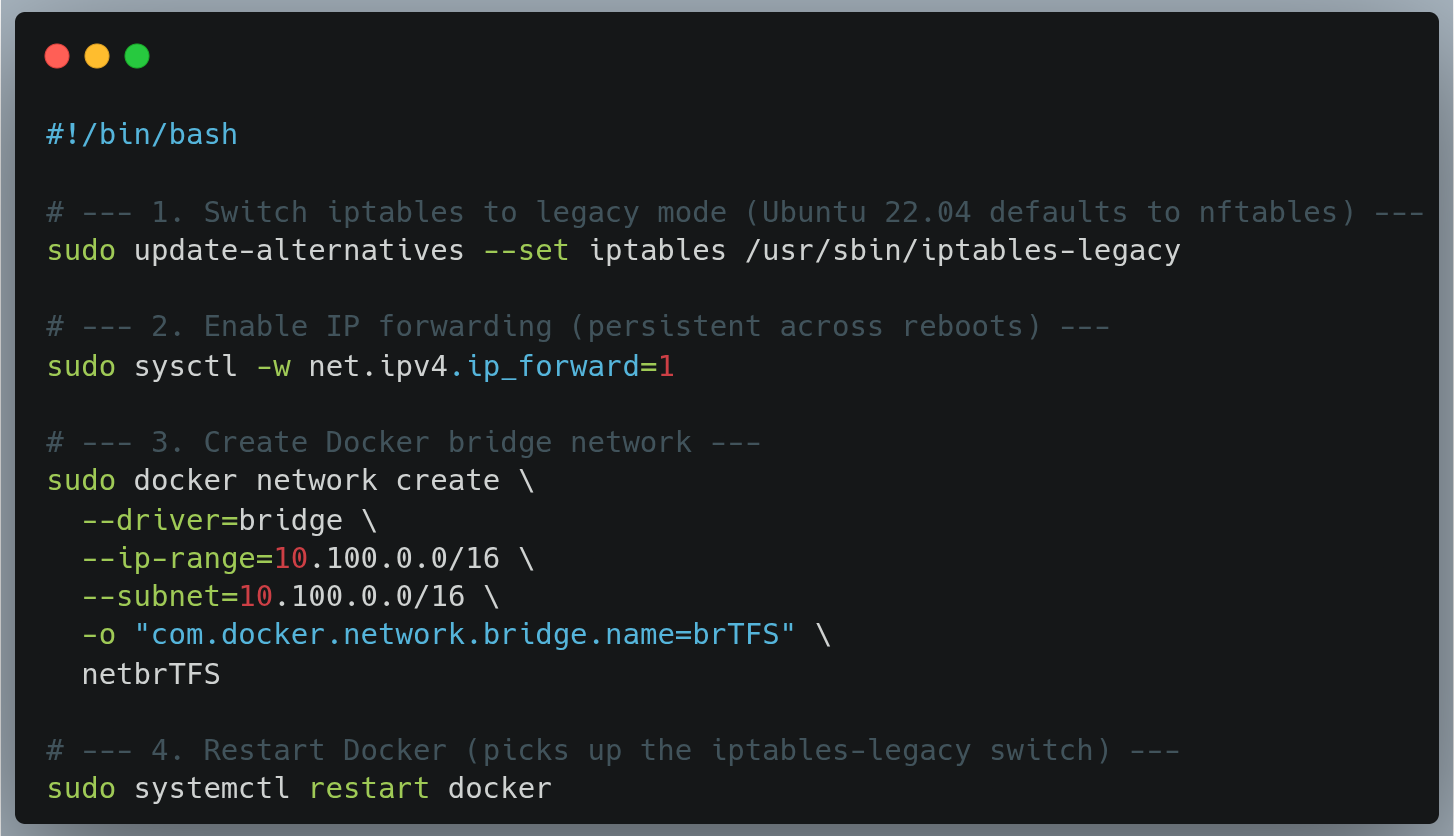
\includegraphics[width=0.8\textwidth]{setup_network.png}
    \caption{Virtual network for the emulated devices}
    \label{fig:setup_network}
\end{figure}
To resolve this and establish cross-server connectivity, a dedicated virtual network is provisioned on the secondary server. To standardize the deployment, this configuration is abstracted into two automated scripts provided within the repository. Initially, the~\emph{setup\_network.sh} script according to Fig.~\ref{fig:setup_network} is executed to revert the host environment to~\emph{iptables-legacy}, enable kernel-level IP forwarding, and provision the isolated Docker bridge (designated as brTFS).
\begin{figure}[htbp]
    \centering
    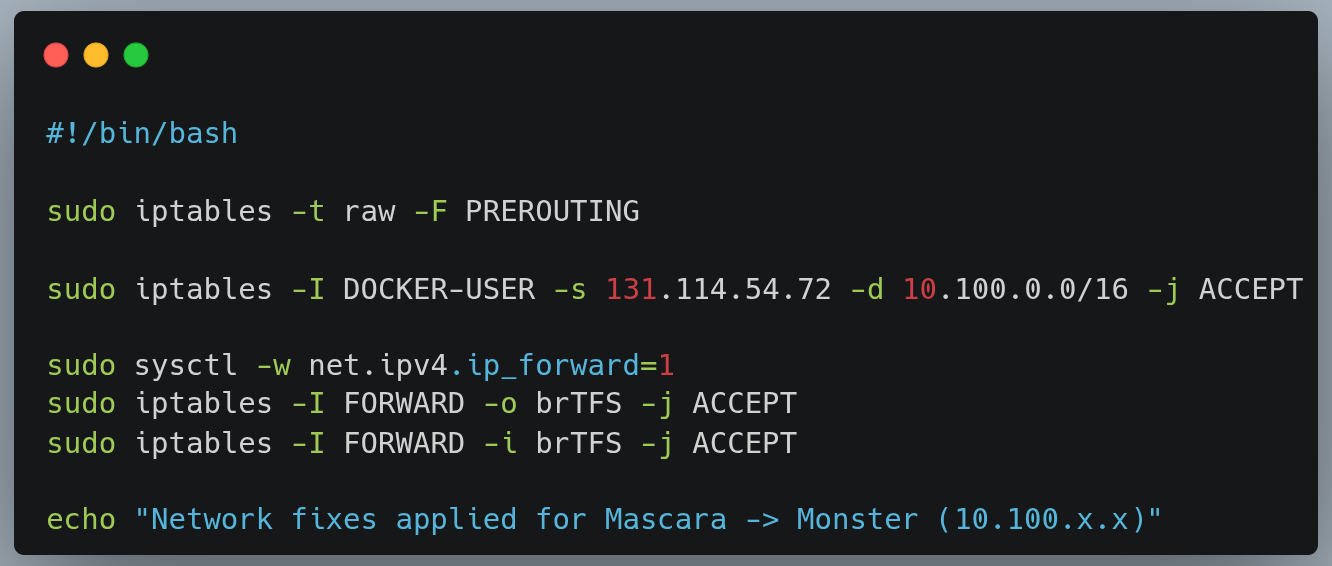
\includegraphics[width=0.8\textwidth]{fix_connectivity.png}
    \caption{Add exceptions to the firewall}
    \label{fig:fix_connectivity}
\end{figure}
Furthermore, because dynamic container generation frequently alters active network chains, persistent routing must be enforced iteratively. To achieve this, according to Fig.~\ref{fig:fix_connectivity} the~\emph{fix\_connectivity.sh} script is executed each time a new topology is generated. This secondary script injects targeted firewall exceptions into the~\emph{DOCKER-USER} and~\emph{FORWARD} chains, ensuring the primary server maintains uninterrupted access to the emulated devices.

\subsection{Emulated Devices}
The emulation environment provisions two fundamental classes of optical equipment: muxponders, which function as optical terminal endpoints, and ROADMs. The container images leverage established research-based repositories, providing a robust baseline for simulating optical behavior.
\begin{figure}[htbp]
    \centering
    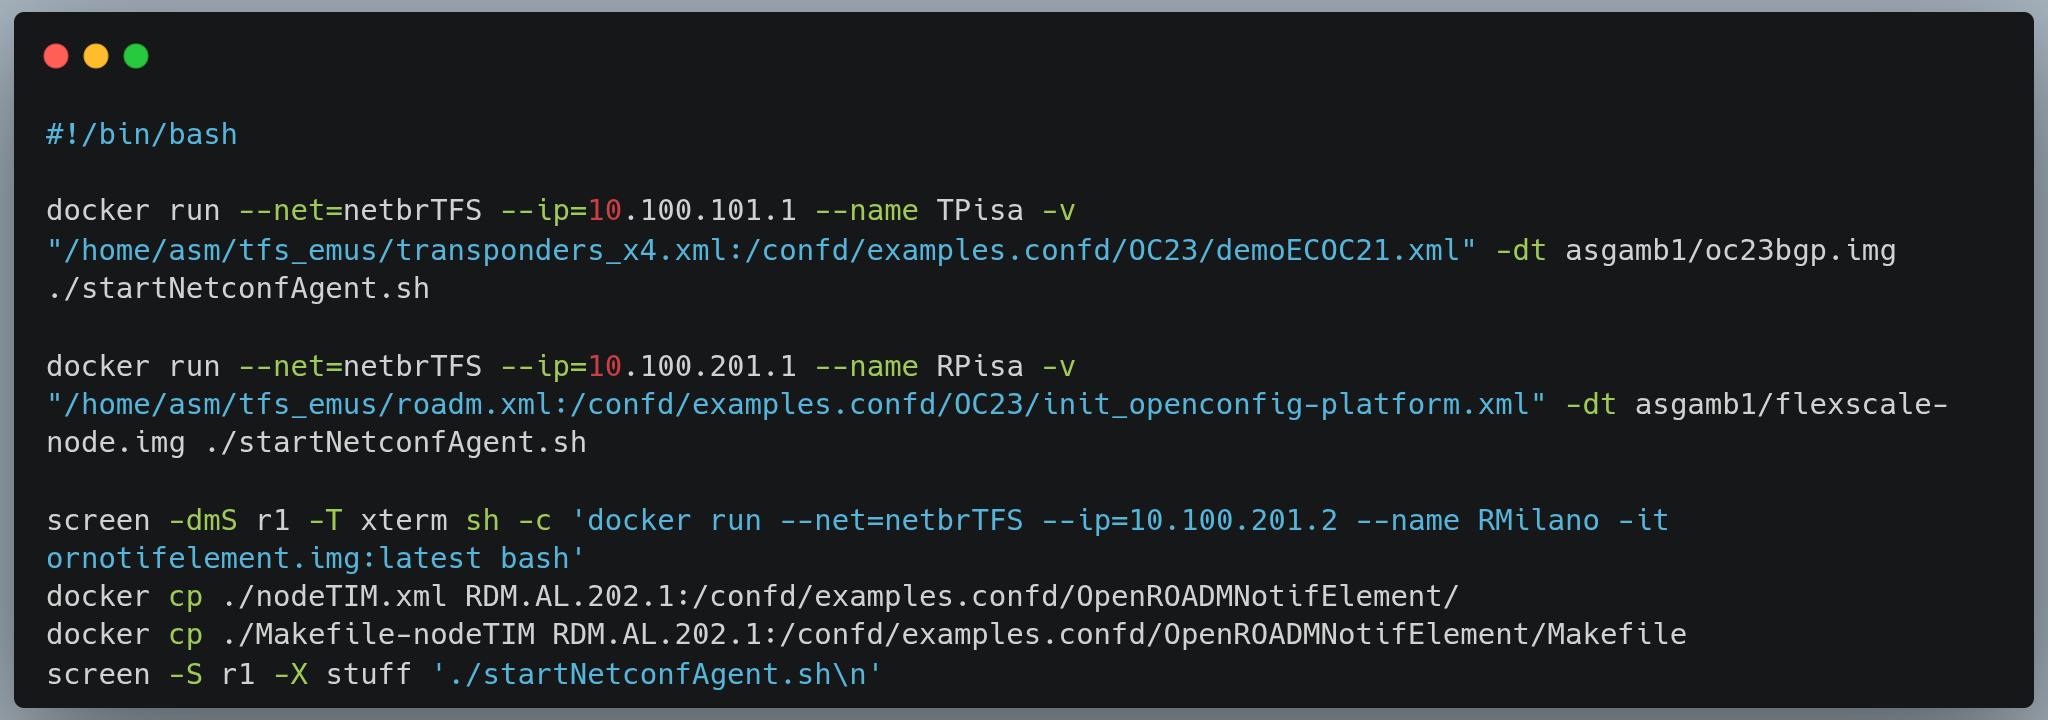
\includegraphics[width=0.8\textwidth]{emulated_devices.png}
    \caption{Add exceptions to the firewall}
    \label{fig:emulated_devices}
\end{figure}
According to the bash script in Fig.~\ref{fig:emulated_devices} each emulator is instantiated within the dedicated~\emph{netbrTFS} bridge network with a static IP address to ensure reachability across the testbed. During the container initialization process, essential configuration files—modeled on standardized~\emph{OpenConfig} and~\emph{OpenROADM} YANG data structures—are injected into the container's environment. These XML payloads serve as the device's persistent state, which is subsequently exposed and managed by the SDN controller via the~\emph{NETCONF} protocol. This configuration workflow allows the emulated hardware to accurately reflect the operational properties of physical optical networking elements, such as port configurations, frequency ranges, and transceiver's capabilities.

\subsection{Test Topology}
The performance evaluation was conducted across two distinct network topologies, NSFNET and PANEU; however, the PANEU reference model is analyzed here to illustrate the configuration workflow. As illustrated in Fig.~\ref{fig:pan_eu_org}, the PANEU topology comprises 27 nodes and 55 bi-directional links. For the purposes of this evaluation, the nodes are configured as ROADMs, supplemented by a set of muxponders connected as terminal endpoints. This topology provides a robust framework for assessing the scalability and efficiency of the RSA algorithm under realistic network loads. A detailed analysis of the resulting simulation performance, including statistical evaluation and comparative throughput metrics, is provided in the subsequent chapters.
\begin{figure}[htbp]
    \centering
    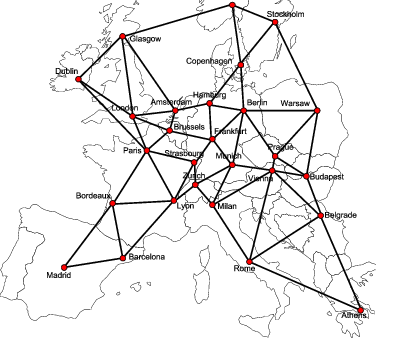
\includegraphics[width=0.6\textwidth]{pan_eu_org.png}
    \caption{Referenced Pan-European network topology~\cite{4814809}}
    \label{fig:pan_eu_org}
\end{figure}
To generate the topology within TFS the following steps are to be performed consecutively:
\begin{enumerate}
    \item \textbf{Creating Nodes:} To simulate the network environment, the deployment executes the automated script~\verb|allGenerate.sh|, located within the~\verb|main/test/paneu_nsf| directory of the dedicated repository~\cite{pocgit}. This script programmatically instantiates the required topology, including all emulated muxponders and ROADMs, as isolated Docker container instances. Once these containers are fully operational, network reachability must be verified. This validation is performed by issuing standard ICMP ping requests from the primary server directly to the management IP addresses of the newly provisioned devices. Confirming this bidirectional data path ensures that the high-level orchestration plane can reliably communicate with the underlying emulation layer before testing begins.
    \item \textbf{Service Verification} On the primary server, launch a terminal session and execute the following command to confirm that all required TFS microservices are in an active and healthy state:~\verb|watch -n 1 kubectl get all --all-namespaces|.
    \item \textbf{Base Context Generation:} Within the TFS ecosystem, the primary administrative domain is designated as the admin context. While the architecture supports multiple logical contexts to achieve multi-tenancy, each domain operates relative to this root system-level context. Therefore, the initialization pipeline requires configuring the admin context as the foundational step. To execute this operation, it is necessary to navigates to the TFS WebUI at~\verb|http://primary_server_ip/webui| and uploads the~\emph{adminContext.json} configuration file. These JSON files, formally referred to as TFS descriptors, programmatically define the properties and configurations of a given network function.
    \item \textbf{Topology Generation:} Following the context initialization, the network topology is established by sequentially uploading two distinct JSON descriptors:~\emph{pan\_single.json \& paneu\_parallel.json}. This sequential ingestion allows the controller to progressively build and register the network elements. Upon successful processing of these descriptors, the TFS control plane dynamically visualizes the structural layout of the parallel optical network, matching the reference architecture illustrated in Fig.~\ref{fig:paneu_parallel}.
\end{enumerate}

\begin{figure}[htbp]
    \centering
    \includegraphics[width=0.8\textwidth]{paneu\_parallel.png}
    \caption{PANEU topology with non-uniform parallel links within TFS}
    \label{fig:paneu_parallel}
\end{figure}
\begin{figure}[htbp]
    \centering
    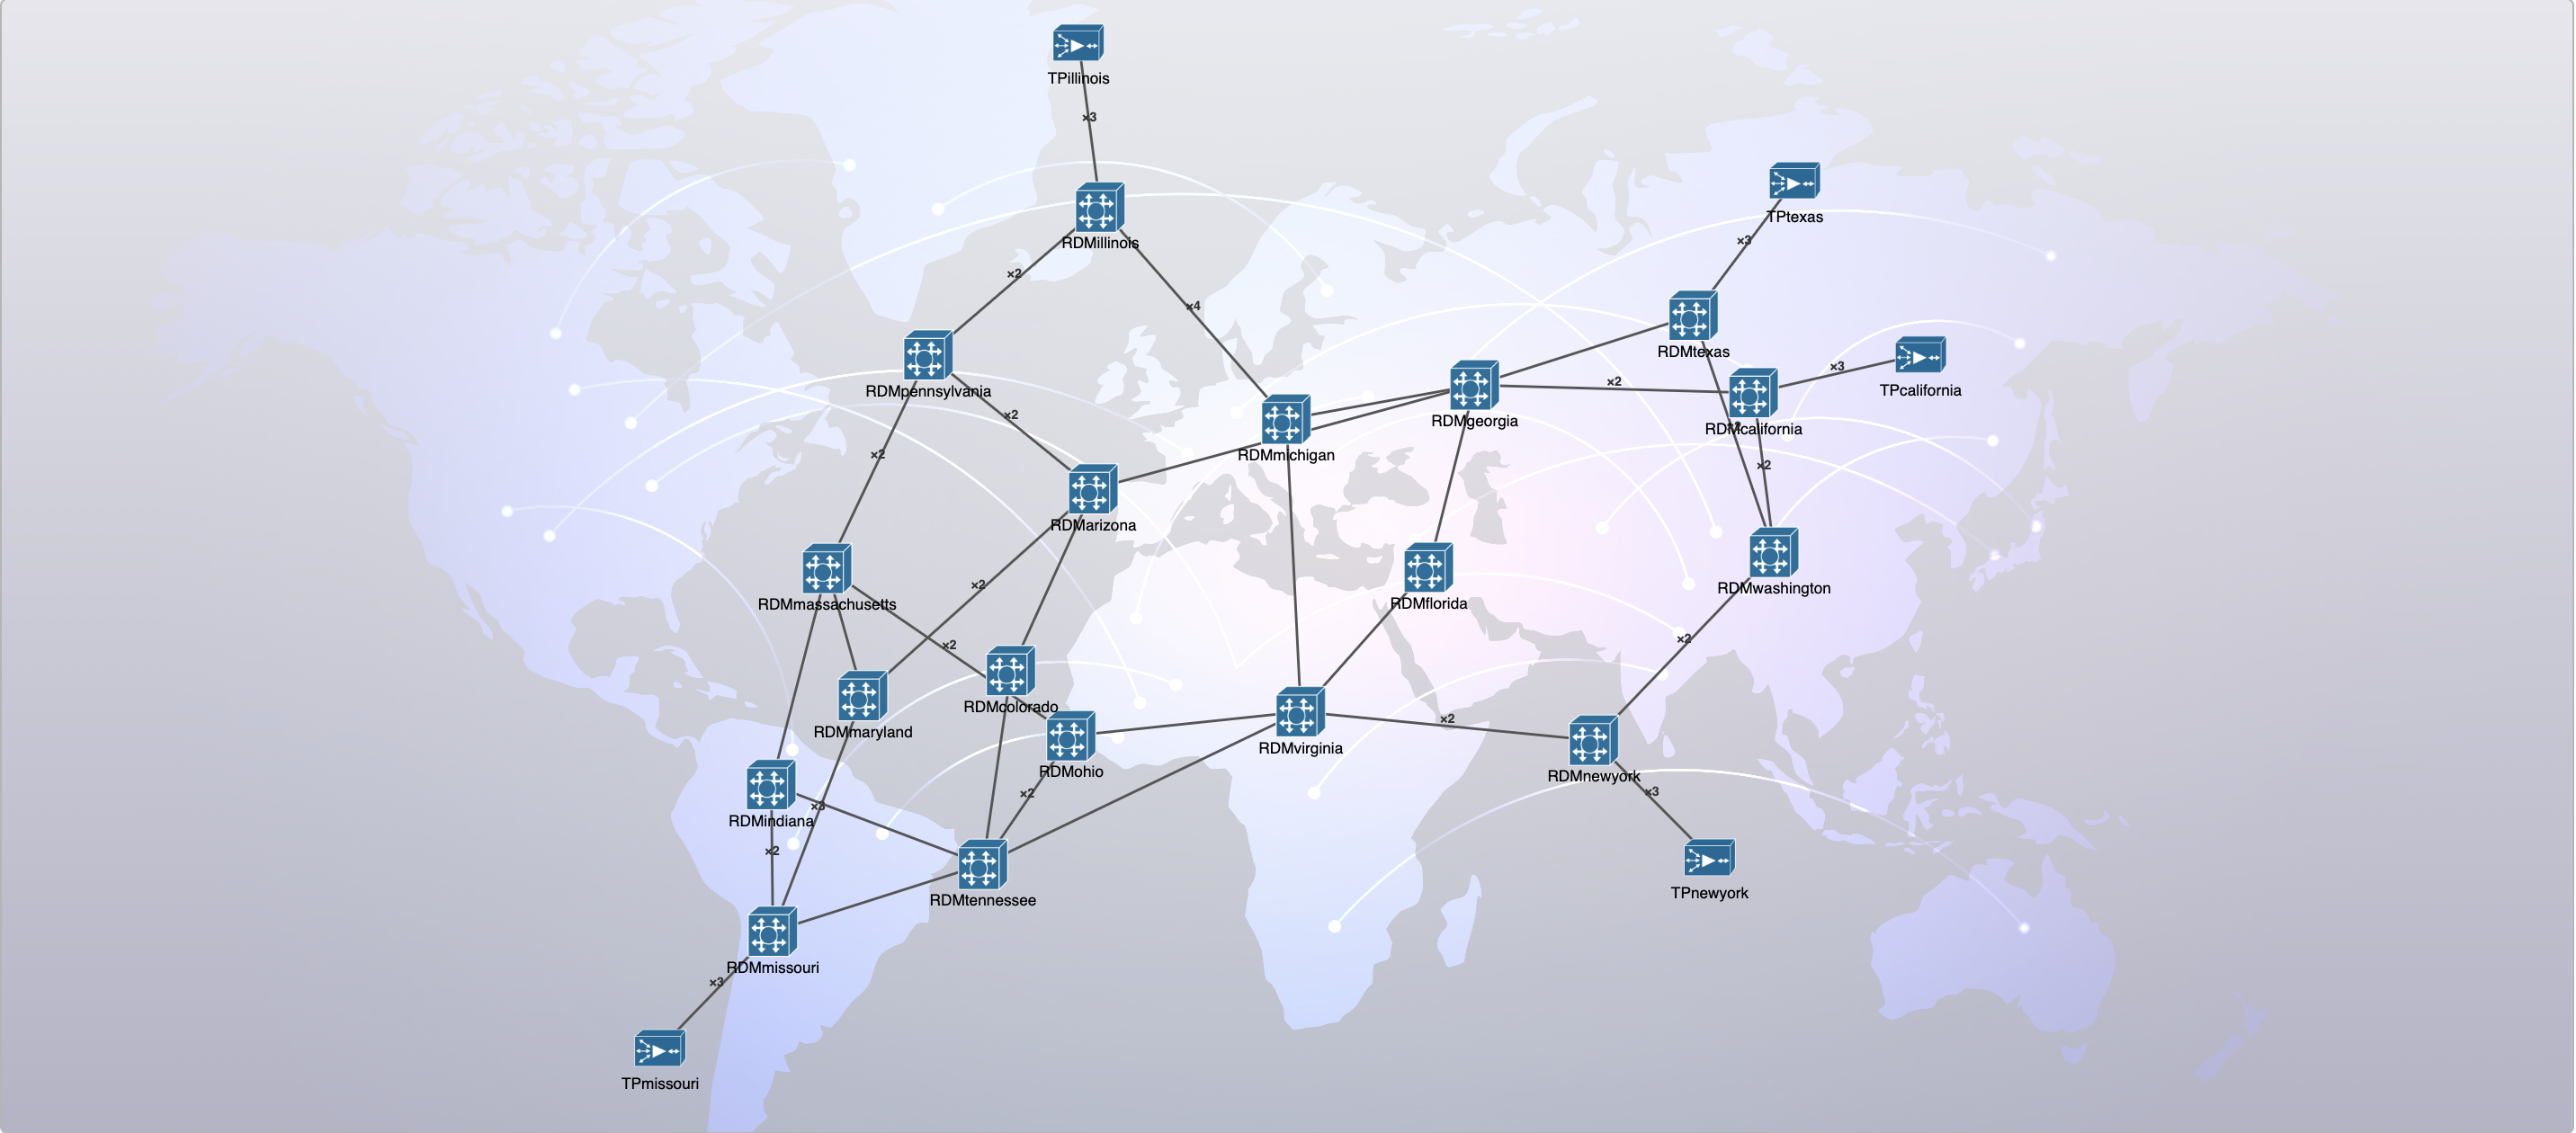
\includegraphics[width=0.8\textwidth]{nsf_parallel.png}
    \caption{NSFNET topology with non-uniform parallel links within TFS}
    \label{fig:nsf_parallel_topo}
\end{figure}

\chapter{Results and Evaluation}
This chapter presents a comprehensive performance evaluation and functional validation of the proposed RSA framework. To substantiate the theoretical claims established in preceding chapters, the newly integrated POC is rigorously tested within the TFS ecosystem across a variety of reference topologies. The subsequent sections provide an in-depth assessment of the system's operational success, systematically analyzing its computational performance and algorithmic efficiency. Furthermore, this chapter details network throughput metrics, conducts a statistical analysis of path blocking probabilities, and presents a direct comparative evaluation.

\section{Evaluation Methodology \& Test Scenarios}
The evaluation methodology injects dynamic optical intents into the TFS control plane, and it systematically monitors the system's operational responses. The test scenarios evaluate the system across various network architectures, and they specifically focus on complex multi-graph configurations. The primary objectives of these comprehensive evaluations are threefold:
\begin{enumerate}
    \item To validate the functional correctness of the dynamic device configuration extraction.\item To measure the computational latency and efficiency of the proposed heuristic.
    \item To analyze path blocking probabilities statistically under varying simulated traffic loads.
\end{enumerate}
Testing was conducted across three distinct network topologies, and each model exhibits varying degrees of node density. To explicitly demonstrate multi-fiber capabilities, each topology was evaluated in a baseline~\emph{Single} configuration alongside a dense~\emph{Parallel} configuration. The specific topologies utilized are as follows:
\begin{itemize}
    \item \textbf{Linear Topology:} A standard point-to-point chain comprises 6 nodes. The single version utilizes 5 links, and the parallel version utilizes 13 links.
    \item \textbf{NSFNet Topology:} A reference model of the National Science Foundation Network comprises 14 nodes. The single configuration ($NSF_s$) features 22 bi-directional links, and the parallel configuration ($NSF_p$) expands to 66 links via a $3\times$ multiplier between each node pair.
    \item \textbf{PANEU Topology:} A highly meshed European network model comprises 27 nodes. The single configuration ($PANEU_s$) features 55 bi-directional links, and the parallel configuration ($PANEU_p$) expands to 165 links via a $3\times$ multiplier.
\end{itemize}
Computational performance and functional correctness were assessed across all three topologies within the TFS environment. However, the subsequent statistical analysis focused exclusively on the NSFNet and PANEU models. These complex models better represent real-world optical networks, and they effectively demonstrate heavy traffic behaviors. Furthermore, this specific statistical simulator was developed entirely outside the TFS ecosystem. This external execution strategically bypassed internal framework communication, and it successfully avoided inter-service latency during mass simulations.

\section{Functional Validation}
Before evaluating quantitative metrics, the functional correctness of the integrated system must be verified. This section validates the operational lifecycle of the POC microservice by cross-referencing backend execution logs directly with the enhanced TFS WebUI. Through this approach, we verify the execution of core features engineered for parallel multi-fiber links, including dynamic hardware configuration extraction, flexible-grid slot mapping, and spectrum assignment table generation. Presenting these backend log excerpts alongside the visual interface elements definitively confirms that the control plane visualization matches the underlying database state and bitmap-based algorithmic computations.

\subsection{ Device info extraction}
As illustrated in Fig.~\ref{fig:web_view_device_info}, this visualization confirms that the extracted granular parameters successfully propagate through the ContextService to be accurately rendered on the operator dashboard.
\begin{figure}[htbp]
    \centering
    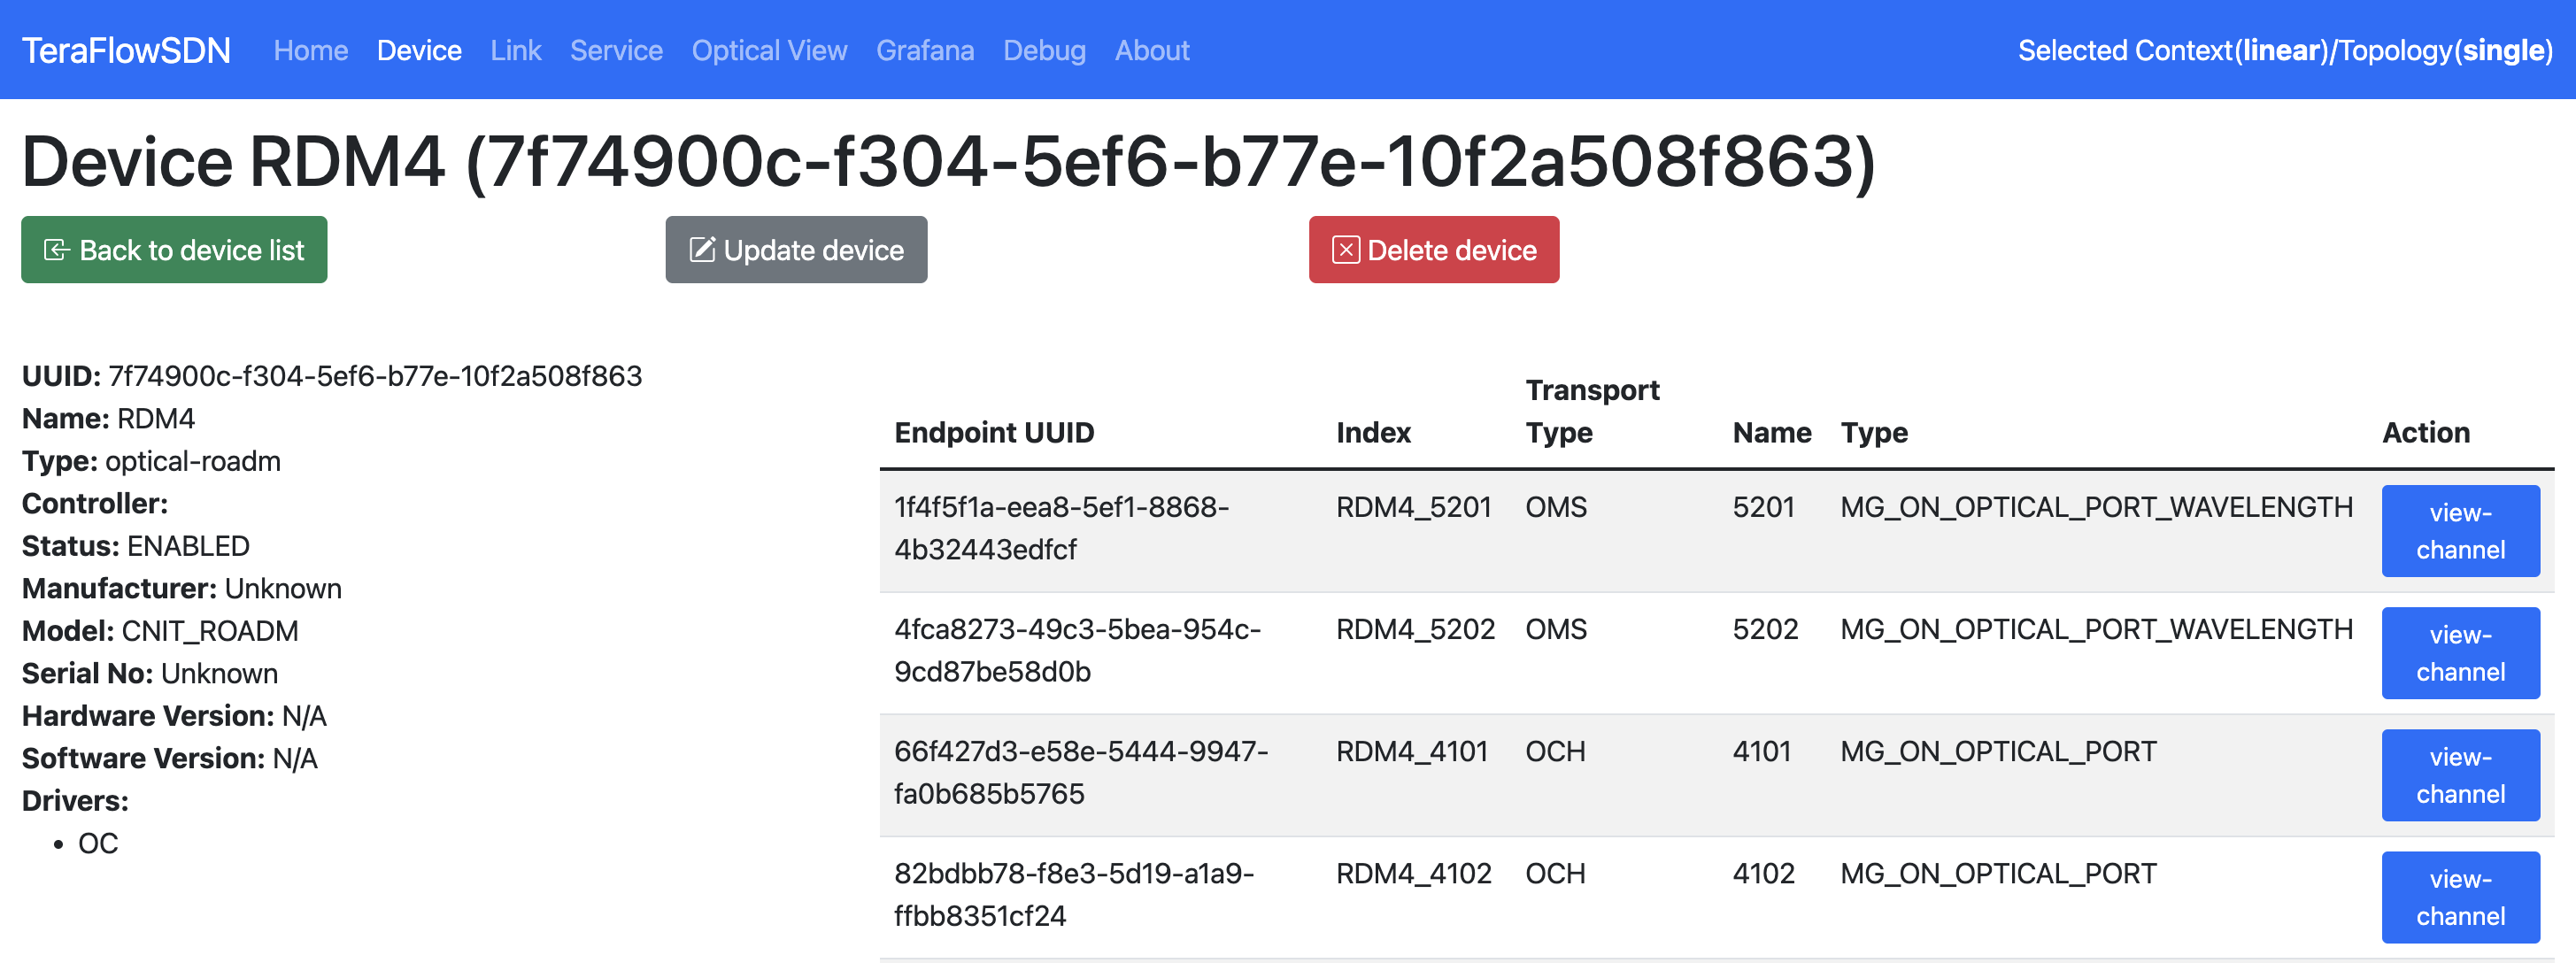
\includegraphics[width=0.8\textwidth]{web_view_device_info.png}
    \caption{An internal configuration of a ROADM device in TFS WebUI}
    \label{fig:web_view_device_info}
\end{figure}
Correspondingly, the execution log verifies the enhancements implemented within the OCDriver to extract dynamic device configurations. This output validates the architectural design, demonstrating that the data extraction methodology dynamically adapts based on the hardware vendor and device model identified during initialization. As illustrated by the workflow in Fig.~\ref{fig:device_info_extraction}, the OCDriver first identifies the specific device model before applying the corresponding filter profile to parse the hardware information.
\begin{figure}[htbp]
    \centering
    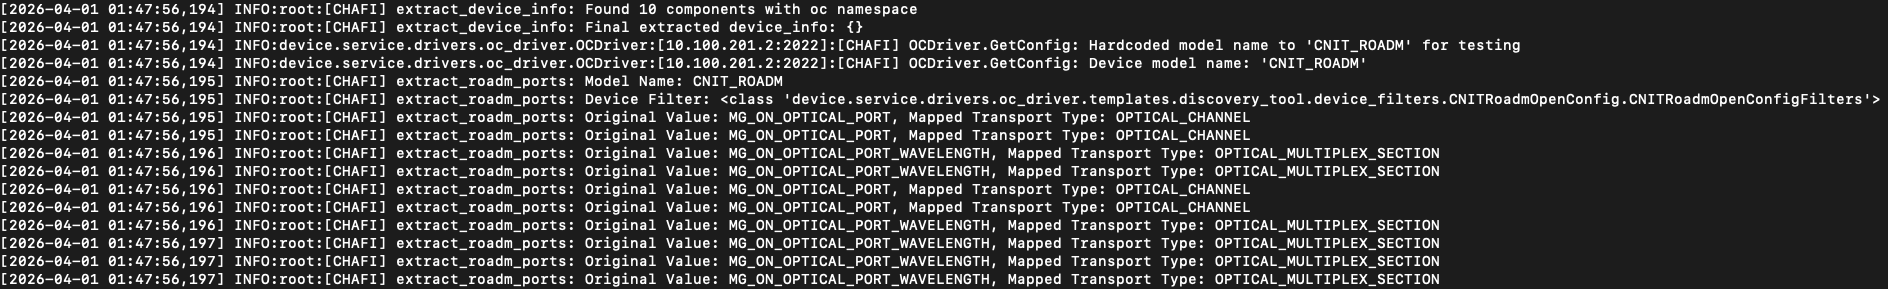
\includegraphics[width=0.8\textwidth]{device_info_extraction.png}
    \caption{Device info extraction using OCDriver}
    \label{fig:device_info_extraction}
\end{figure}
According to Fig.~\ref{fig:frequency_mapping_roadm_ports}, it is visible that the algorithm identifies the highest range of frequencies among all nodes and then expands based on that range. For this particular test, each band (S,C,L) is reduced to 20 slots only.
\begin{figure}[htbp]
    \centering
    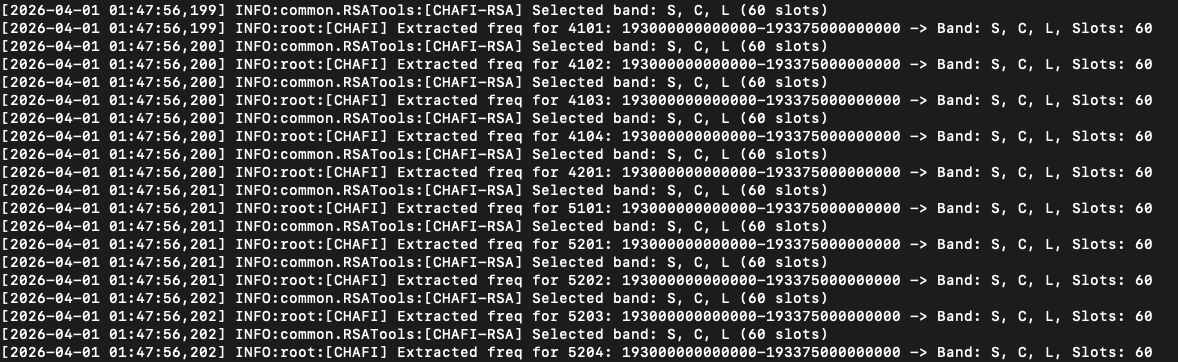
\includegraphics[width=0.8\textwidth]{frequency_mapping_roadm_ports.png}
    \caption{Frequency mapping of the device endpoints}
    \label{fig:frequency_mapping_roadm_ports}
\end{figure}
Finally, in Fig.~\ref{fig:port_rsa} we can see that each slot is visualized based on their availability in TFS WebUI.
\begin{figure}[htbp]
    \centering
    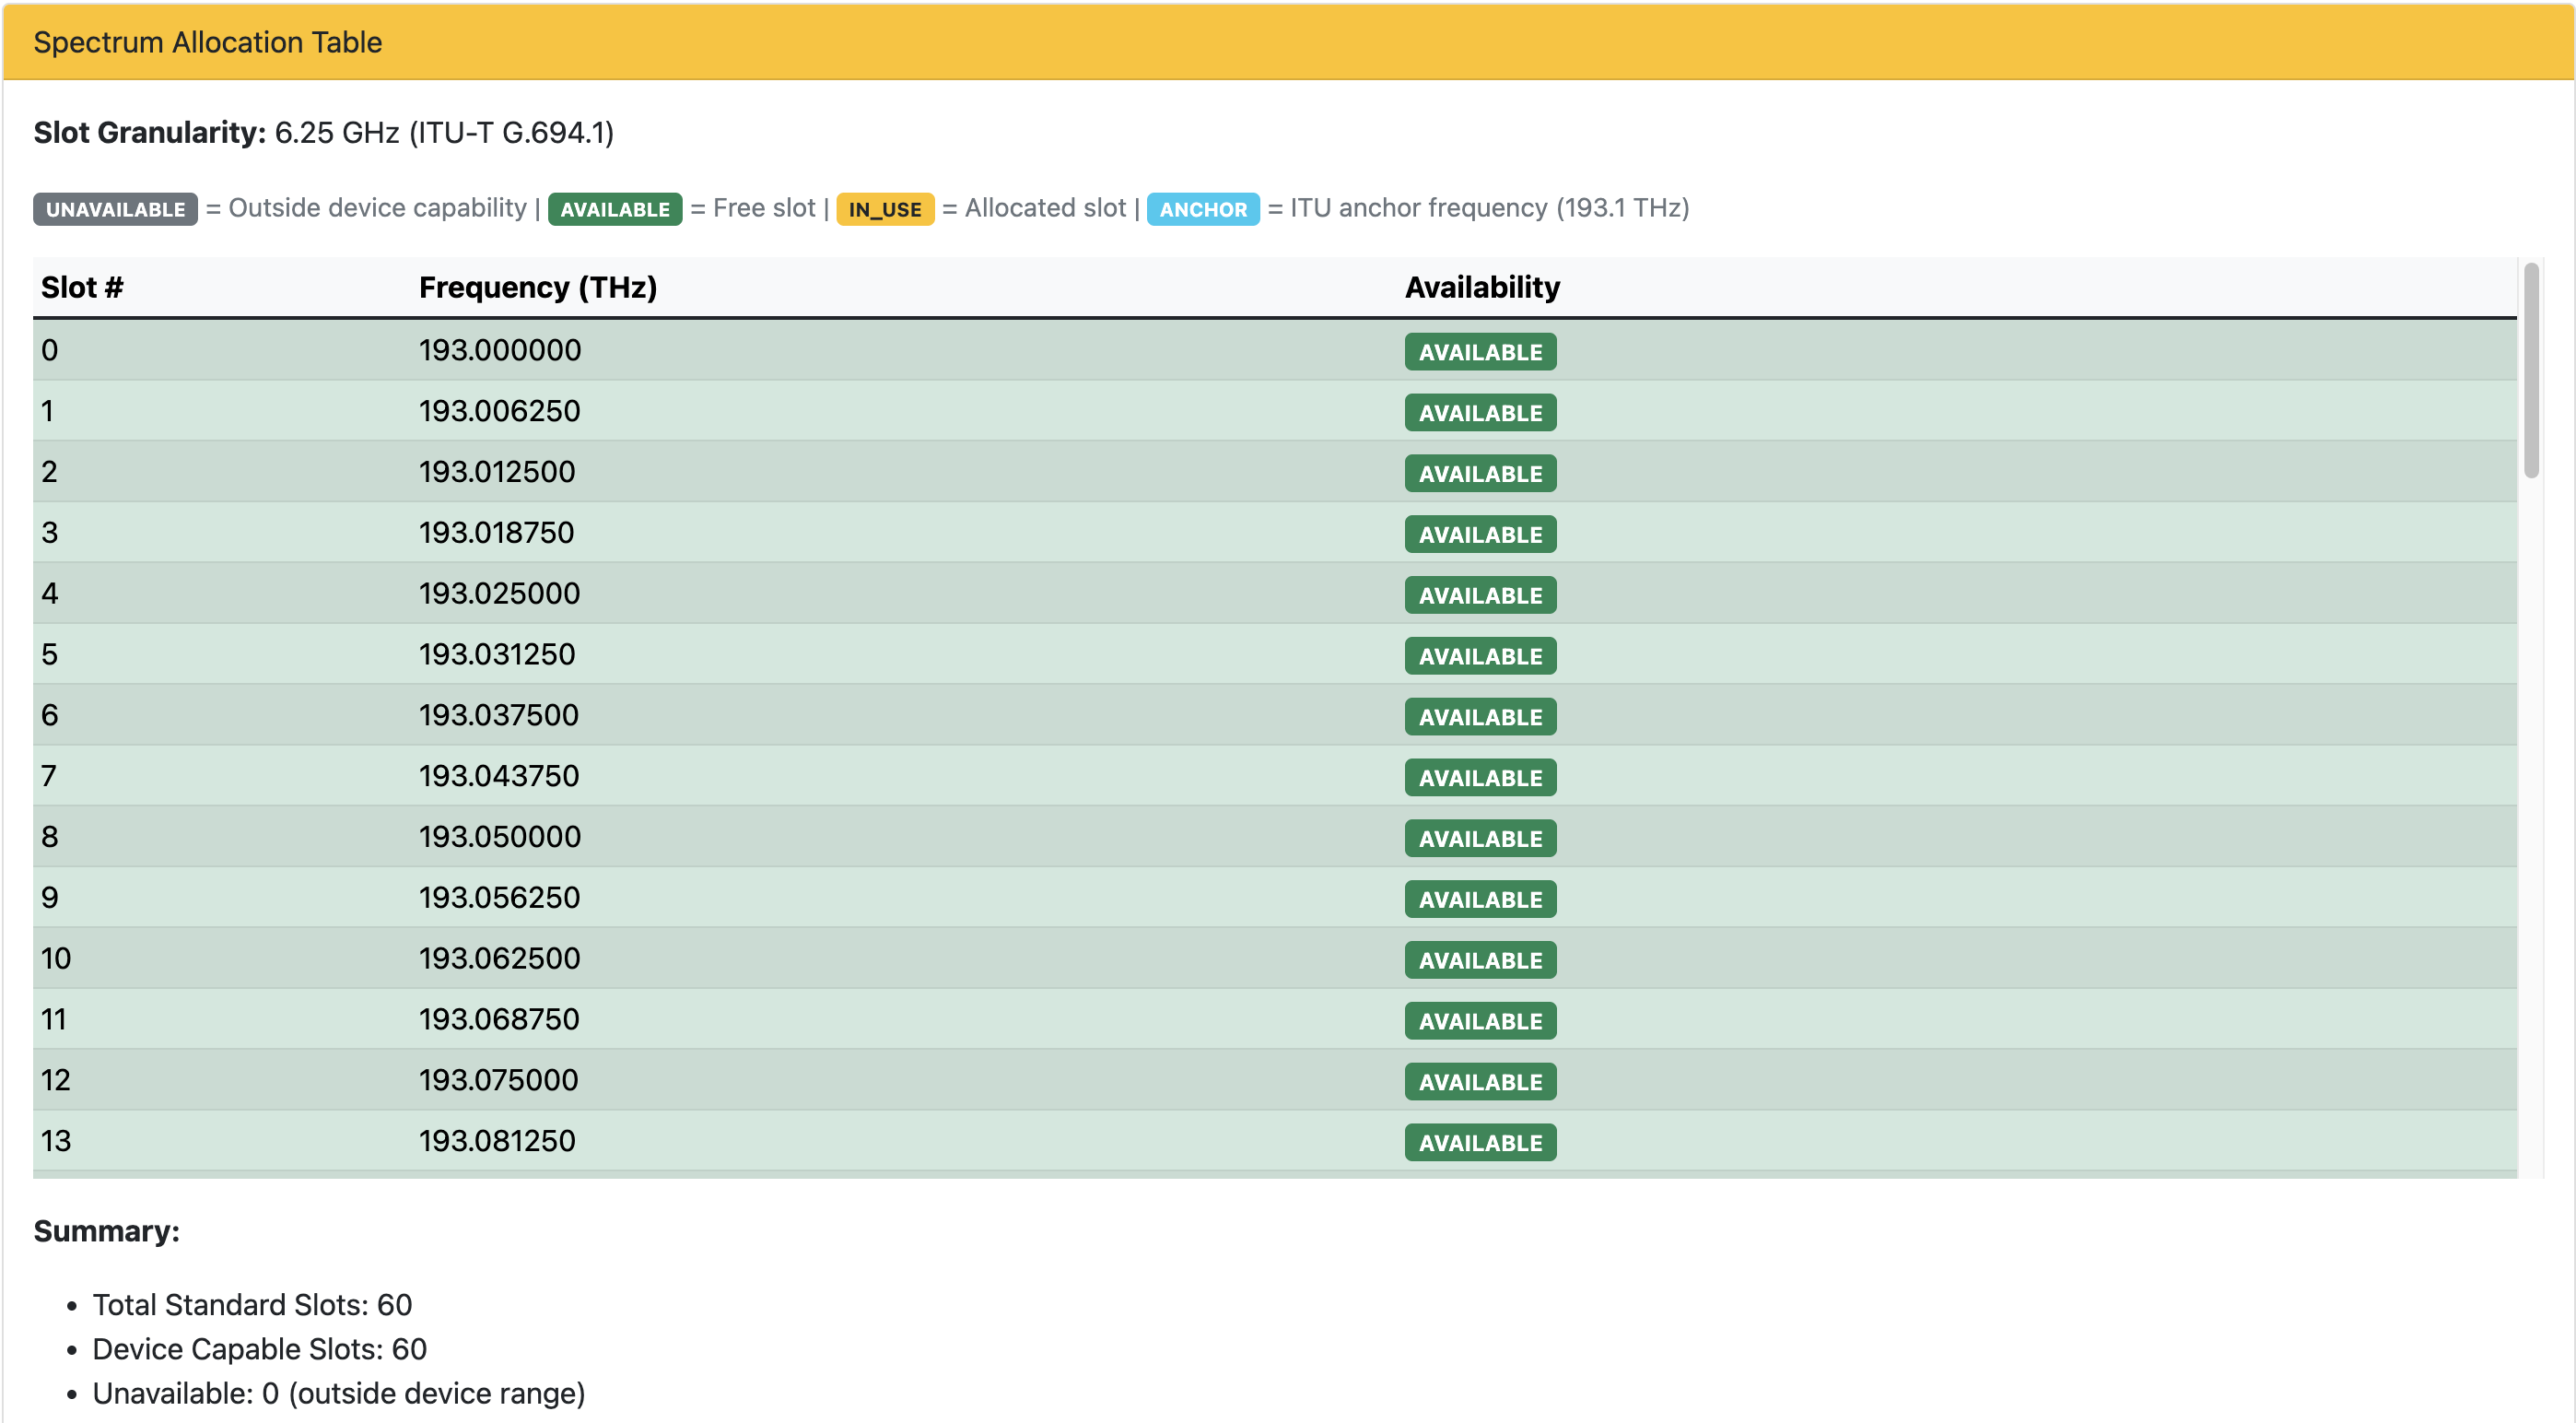
\includegraphics[width=0.8\textwidth]{port_rsa.png}
    \caption{Frequency details of an Endpoint}
    \label{fig:port_rsa}
\end{figure}
\subsection{Link RSA Comparison}
Fig.~\ref{fig:link_rsa} validates the effectiveness of the POC's RSA algorithm by presenting a direct visual comparison of link spectrum utilization. In a multi-fiber network, managing frequency continuity across parallel physical links is computationally challenging. The proposed bitmap-based approach addresses this by dynamically evaluating all available spatial dimensions simultaneously to identify suitable, contiguous spectrum gaps.
\begin{figure}[htbp]
    \centering
    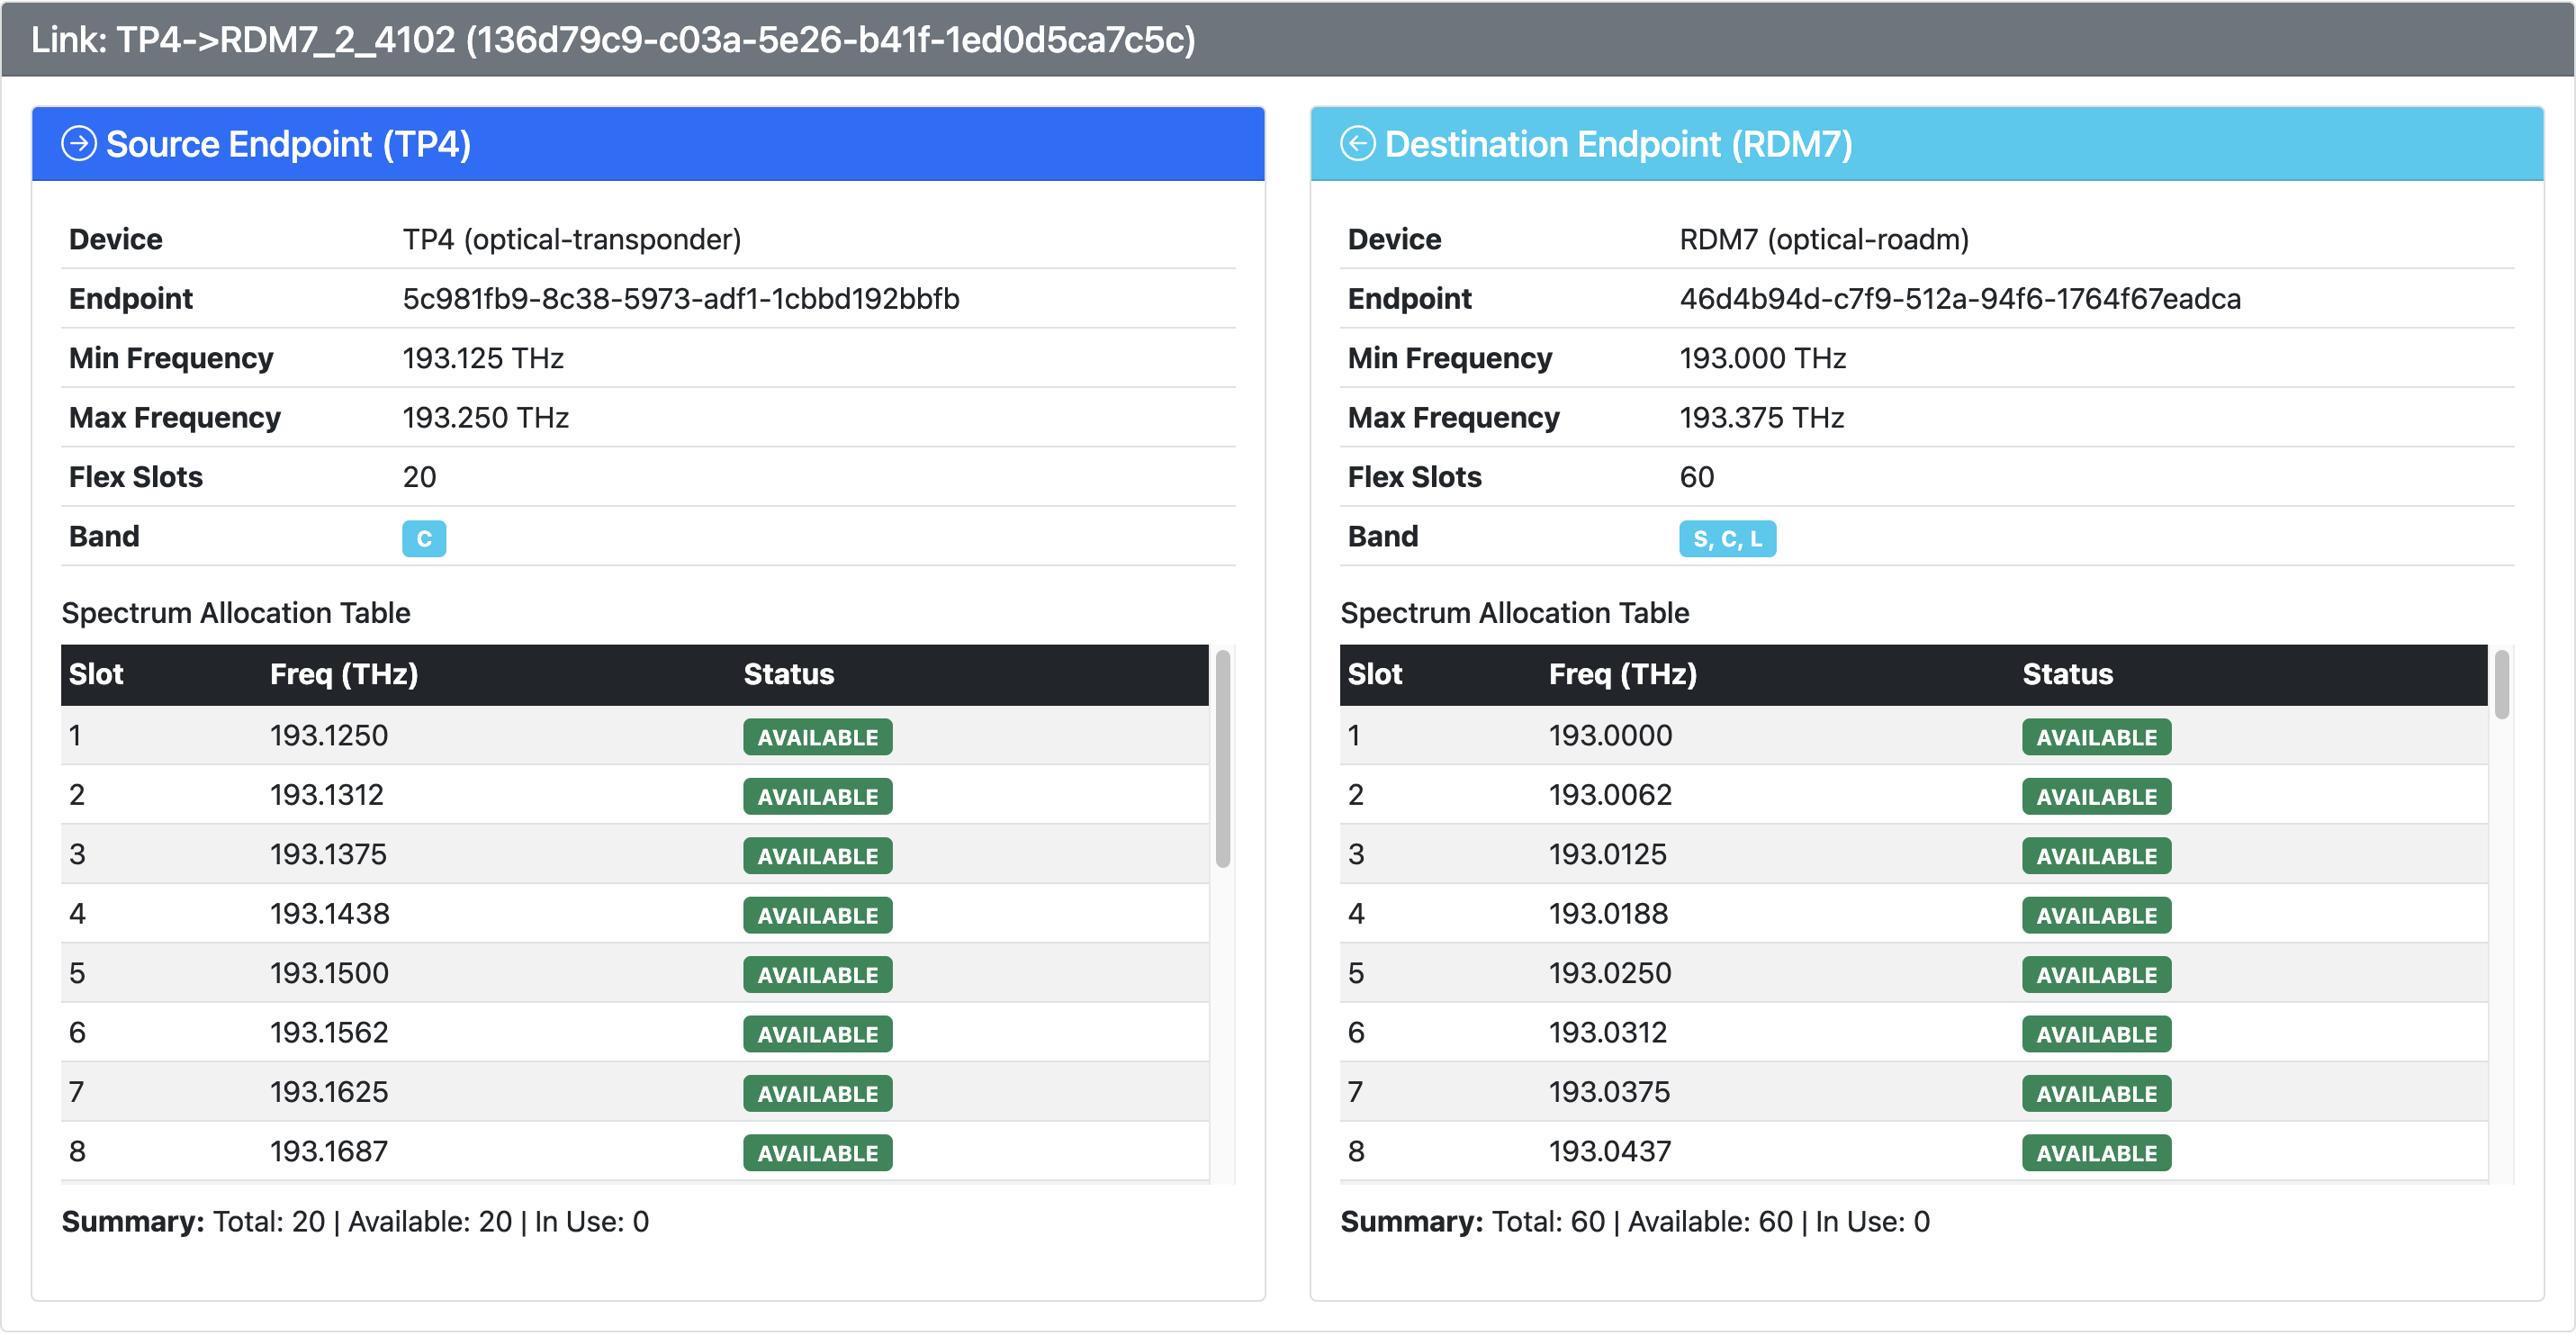
\includegraphics[width=0.8\textwidth]{link_rsa.png}
    \caption{Bitmap of two devices linked by a single fiber}
    \label{fig:link_rsa}
\end{figure}
\subsection{ Optical Intent or Lightpath }
The optical intent or lightpath request in TFS ecosystem is treated as a special service functional as~\emph{OPTICAL\_CONNECTIVITY}. To avail this service, the operator must upload a well strcuted JSON descriptor through the WebUI. Upon receiving the optical connectivity service request, the~\emph{ServiceServicer} microservice reveals this request to the POC. As shown in Fig.\ref{fig:optical_connectivity_service} a lightpath request has been activated between to terminla devices~\emph{T1, T2}.
\begin{figure}[htbp]
    \centering
    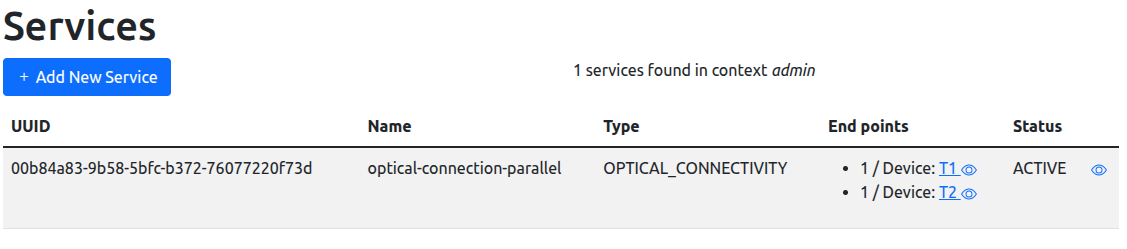
\includegraphics[width=0.8\textwidth]{optical_connectivity_service.png}
    \caption{Optical connectivity service in TFS}
    \label{fig:optical_connectivity_service}
\end{figure}
\subsection{ Spectrum Assignment of a Lightpath}
As shown in Fig.~\ref{fig:shortest_path} the algorithmic execution by tracing a specific lightpath request from initiation to final spectral assignment. The functional validation focuses on the transition from topological path discovery using Dijkstra's algorithm on the simplified graph $(G_s)$ to the bitwise spatial-spectral intersection.
\begin{figure}[htbp]
    \centering
    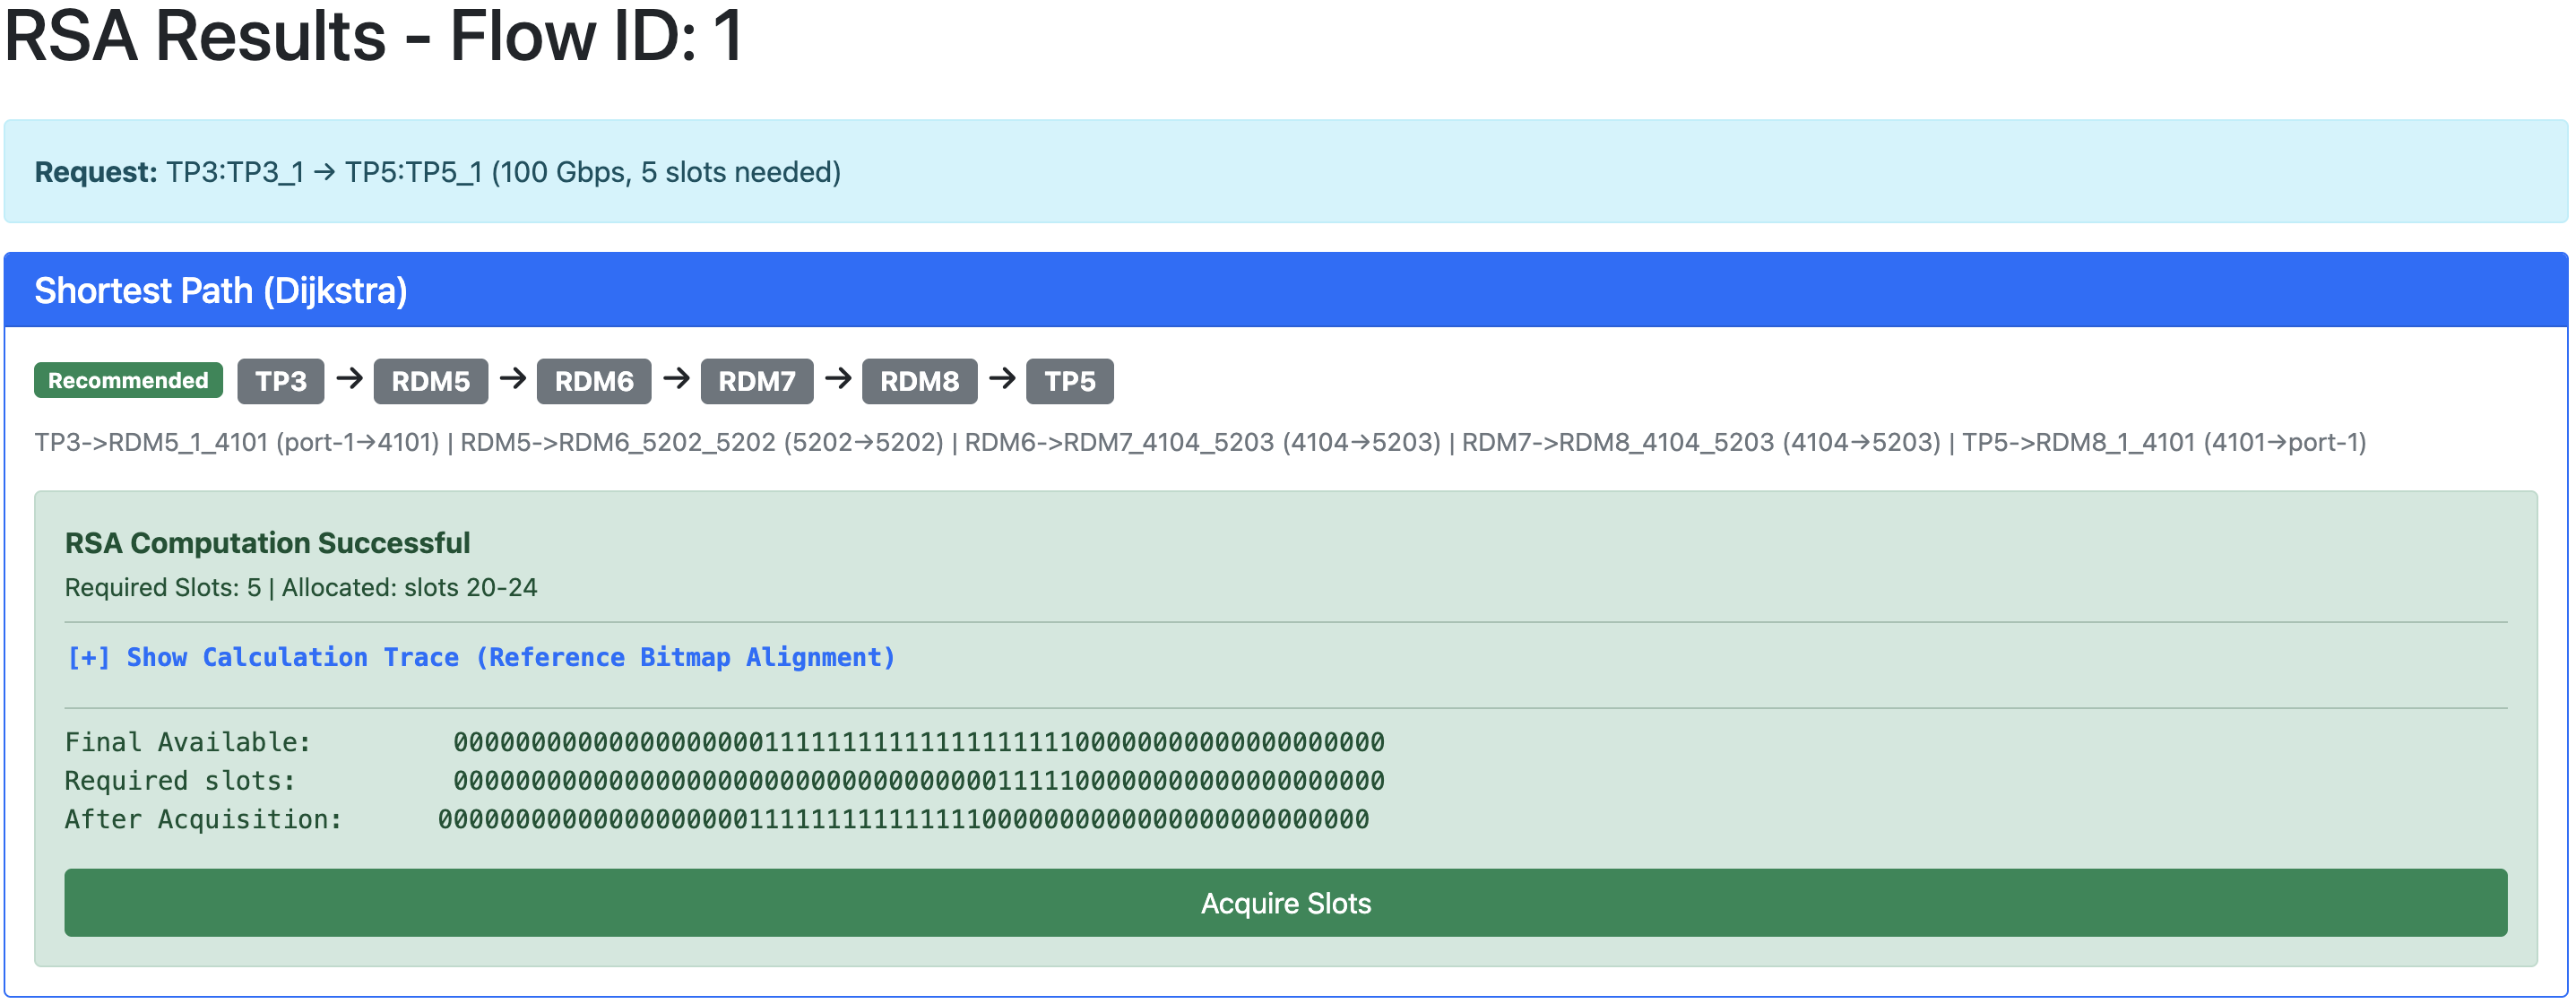
\includegraphics[width=0.8\textwidth]{shortest_path.png}
    \caption{Shortest path discovery}
    \label{fig:shortest_path}
\end{figure}
Following path discovery, the controller executes a hop-by-hop analysis of the spectral state, as illustrated in Fig.~\ref{fig:hop_rsa}. For every add-drop hop, the controller retrieves the occupancy bitmaps of all constituent parallel links and performs a concurrent bitwise intersection. This process collapses the spatial complexity of the multi-fiber bundle into a single, unified availability bitmap, ensuring that the selected contiguous slots are physically vacant across the entire spatial breadth of the path. For intermediate hops, the algorithm adopts a preference-based path selection scheme. A comparative evaluation of these different routing schemes is detailed within the statistical analysis in next sections.
\begin{figure}[htbp]
    \centering
    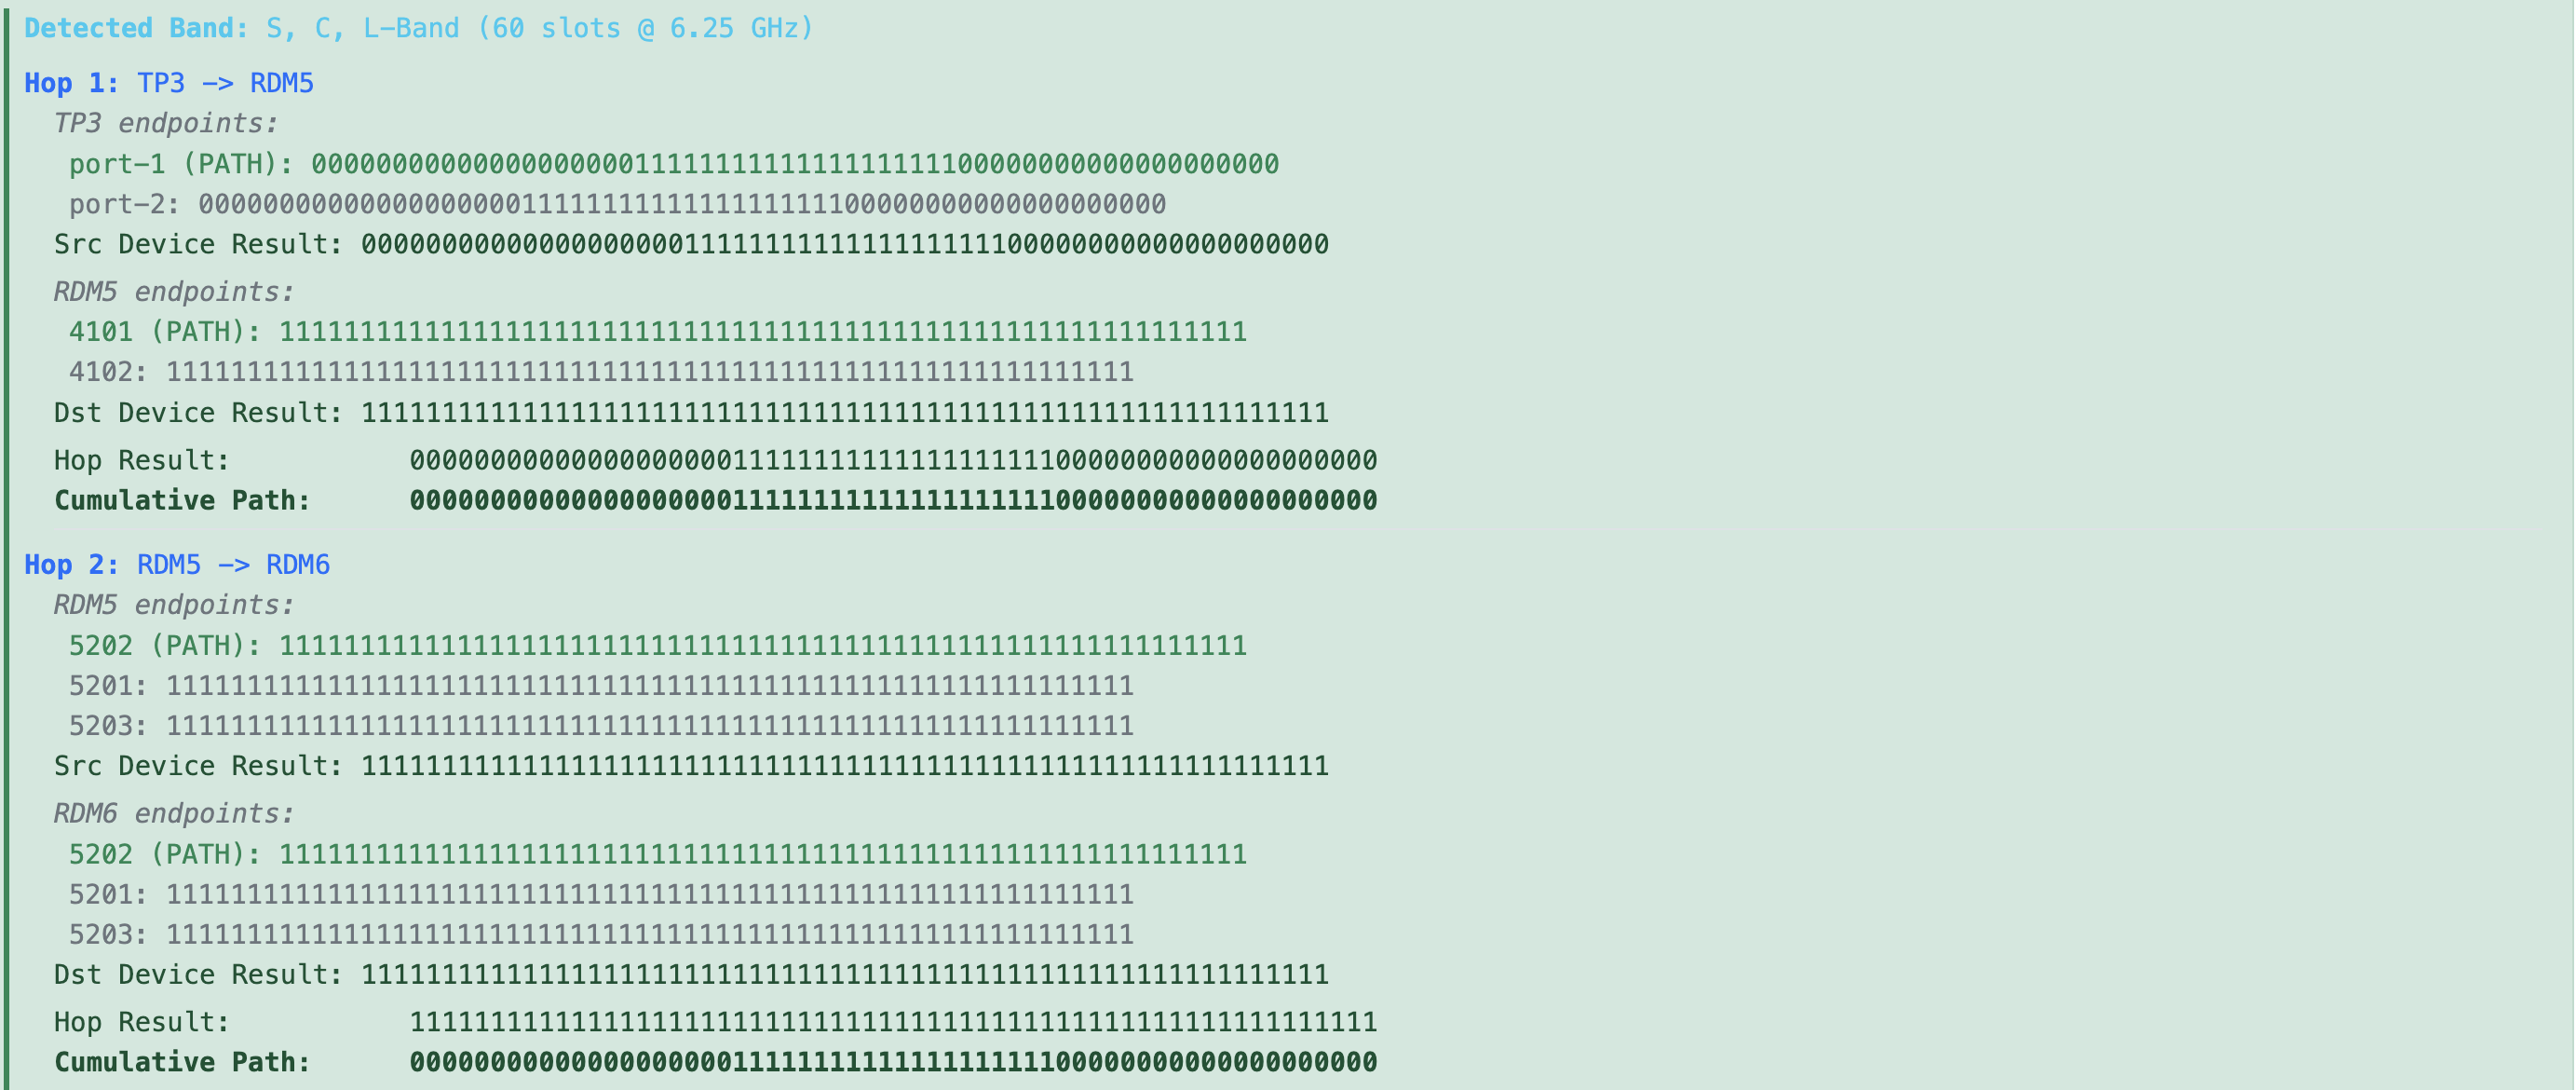
\includegraphics[width=0.8\textwidth]{hop_rsa.png}
    \caption{Hop-by-hop RSA computation}
    \label{fig:hop_rsa}
\end{figure}

\subsection{Additional Path Computation}
Along with the shortest path, the algorithm computes alternative routes based on the constraint~\emph{$\Delta\mathcal{H}$}, which defines the maximum number of additional allowed hops (Fig.~\ref{fig:additional_path}). While these additional paths are theoretically expected to optimize traffic management and balance network load, the empirical statistical analysis reveals a contrary behavior. A comprehensive evaluation of this performance divergence is detailed in the subsequent results chapter.
\begin{figure}[htbp]
    \centering
    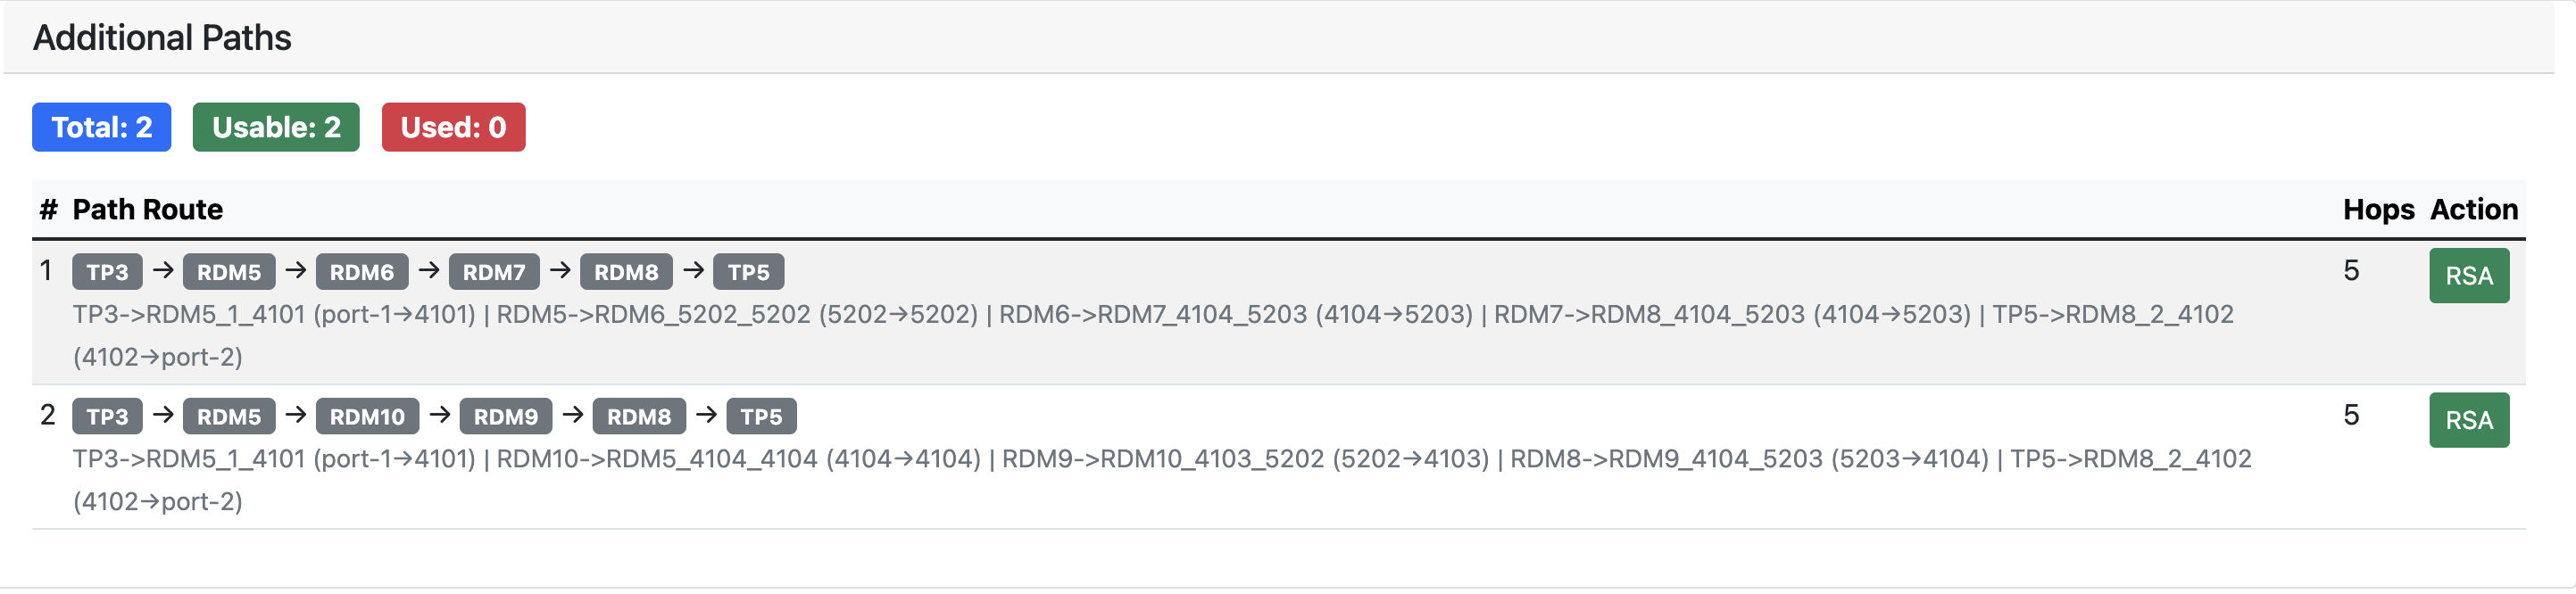
\includegraphics[width=0.8\textwidth]{additional_path.png}
    \caption{Additional Path Computation}
    \label{fig:additional_path}
\end{figure}
\section{Performance Evaluation}
This section presents a quantitative evaluation of the computational latency introduced during the provisioning lifecycle of the POC. To assess algorithmic efficiency and scalability, execution times were benchmarked across three distinct processing phases: Graph Generation (GG), Shortest Path Computation (SPC), and Spectrum Assignment Computation (SAC). The evaluation spans the three previously established reference topologies, with each network analyzed under both a standard single-fiber baseline and a highly dense multi-fiber configuration. All recorded execution metrics are reported in~\emph{seconds}. This analysis ignores the inter service communication delays to demonstrate pure computational latencies.
\begin{table}[htbp]
    \centering
    \begin{tabular}{|c|c|c|c|c|c|}
        \hline
        \textbf{Topology} & \textbf{GG} & \textbf{SPC} & \textbf{SAC} & \textbf{Total Time} & \textbf{Efficiency} \\
        \hline
        Linear Single     & 0.0018      & 0.0012       & 0.0003       & 0.0033              & -                   \\
        \hline
        Linear Parallel   & 0.0018      & 0.0016       & 0.0005       & 0.0039              & 87.50\%             \\
        \hline
        NSF Single        & 0.0019      & 0.0016       & 0.0007       & 0.0042              & -                   \\
        \hline
        NSF Parallel      & 0.0022      & 0.0021       & 0.0011       & 0.0054              & 83.33\%             \\
        \hline
        PANEU Single      & 0.0024      & 0.0024       & 0.0013       & 0.0061              & -                   \\
        \hline
        PANEU Parallel    & 0.0026      & 0.0027       & 0.0019       & 0.0072              & 91.54\%             \\
        \hline
    \end{tabular}
    \caption{Performance Evaluation of POC including Total Execution Time}
    \label{tab:complexity_analysis_table}
\end{table}
The theoretical complexity analysis in~\ref{complexity_analysis} posits that introducing parallel fiber links ($P$) does not scale the worst-case time complexity of the topological routing phase. This efficiency is achieved by decoupling the routing logic from the spatial spectrum allocation. By abstracting redundant physical connections into  $G_s$, SPC utilizing Dijkstra's algorithm is restricted to a time complexity bounded by $\mathcal{O}(KV(L+V\log V))$.

To empirically validate this hypothesis, the total execution time—defined as the summation of Graph Generation ($T_{GG}$), Shortest Path Computation ($T_{SPC}$), and Spectrum Assignment Computation ($T_{SAC}$)—was benchmarked across the Linear, NSF, and PANEU reference models. To quantify the algorithmic scalability when transitioning from a standard single-fiber topology to a dense multi-fiber configuration, a computational efficiency metric ($\varepsilon$) is defined. This metric evaluates the relative temporal performance retained by the controller when processing parallel links, formulated as:

$$\varepsilon=\frac{Time_{single-link}}{Time_{parallel-link}}\times 100$$

Applying this metric to the execution benchmarks reveals critical insights into the controller's scalability across varying topological densities. In the baseline Linear topology, the cumulative execution time increases slightly in the multi-fiber configuration, yielding a high computational efficiency of 87.50\%. The NSF topology demonstrates a comparable but slightly lower efficiency of 83.33\%. Across both of these smaller networks, the $T_{SPC}$ phase experiences a marginal absolute increase (e.g., rising from 0.0012 to 0.0016 seconds in the Linear model, and 0.0016 to 0.0021 seconds in the NSF model). This confirms that the overhead introduced to the pathfinding algorithm by the parallel architecture remains highly constrained.

The most significant substantiation of the algorithm's scalability is observed within the highly complex PANEU topology. Despite the inherent density of 27 nodes and 55 bi-directional links, the PANEU model registers the highest computational efficiency among all tested configurations at 91.54\%. Within this topology, the $T_{SPC}$ execution time increases by merely 0.0003 seconds (from 0.0024 seconds in the single-link configuration to 0.0027 seconds in the parallel configuration).This marginal variance mathematically corroborates the foundational algorithmic claim: the structural abstraction of the network into $G_s$ successfully insulates the core pathfinding operations from increased spatial complexity. Consequently, the absolute temporal increases associated with parallel links are strictly confined to the pre-processing ($T_{GG}$) and post-processing ($T_{SAC}$) phases, POC to maintain robust and highly efficient provisioning performance even as overall network complexity scales.

\section{Throughput Analysis}
While the preceding section analyzed the isolated computational latency of individual algorithmic phases, this section evaluates the aggregate operational capacity of the POC. In the context of the SDN control plane, throughput is critical for evaluating the controller's viability in highly dynamic, real-world network environments where connection requests arrive continuously and require immediate resolution. Within the SDN control plane, throughput is fundamentally defined as the maximum sustainable rate of lightpath provisioning requests the controller can successfully process per unit of time. To mathematically derive this metric, it is first necessary to establish the total computational time, denoted as $T_{\text{total}}$, required to process a single, end-to-end request. Once the aggregate processing latency is established, the control plane throughput, represented by the variable $\lambda$, can be determined through an inverse proportional relationship to the total processing time. Specifically, the throughput is calculated using the following mathematical formulation:
\[
    \lambda=\frac{1}{T_{\text{total}}} \text{ (requests/second)}
\]
For the baseline Linear Single topology, the controller processed requests at a rate of approximately 300 requests per second. When scaling up to the multi-fiber Linear Parallel configuration, throughput remained highly robust at 256 requests per second. Similarly, in the mid-scale NSFNet topology—which serves as a highly representative model for standard wide-area networks—the controller maintained a throughput of 238 requests per second in the single-fiber configuration. When subjected to the dense spatial requirements of the NSF Parallel configuration, the system successfully resolved 185 requests per second. This demonstrates that introducing the massive physical capacity of parallel fibers only marginally diminishes the controller's processing rate, validating the efficiency of the bitwise spatial intersection algorithm and efficient path computation.

As topological complexity approaches the extreme scale of the PANEU network, a natural reduction in control plane throughput is observed due to tshe sheer volume of nodes and interconnected edges. The PANEU Single topology yielded a throughput of approximately 51 requests per second. However, even when operating within the PANEU Parallel environment—the most computationally demanding scenario evaluated, featuring 22 nodes and 110 parallel links—the POC sustained a stable throughput of 138 requests per second.

\section{Statistical Analysis}
The statistical evaluation was conducted considering~\emph{NSFNET \& PANEU} topologies only. Adhering to the ITU-T C-Band flex-grid standard, the spectrum is divided into 350 FSUs featuring specified slot width and central frequency granularity. Experiments were conducted across varying traffic loads using a heterogeneous demand profile: 50\% of connection requests at 100 Gbps (requiring 4 FSUs), 25\% at 200 Gbps (4 FSUs), and 25\% at 400 Gbps (6 FSUs). To perform dynamic traffic simulation, a simulator has been designed using Python's Flask microframework outside the TFS ecosystem. Later, it is containerized using Docker and orchestrated via Docker Compose. Lightpath provisioning requests are dynamically generated following a Poisson process and uniformly distributed among the source-destination pairs. The inter-arrival time and holding time of the lightpath requests are exponentially distributed with an average of $1/\lambda$ and $1/\mu$ seconds, respectively. The load offered to the network in provisioning state condition is expressed in Erlangs as the ratio $\lambda/\mu$.

\subsection{Simulation results}
To simplify the simulation model, several foundational assumptions are established. First, we assume that we have enough terminal devices that can handle the client traffic; consequently, the simulated network nodes represent only the ROADMs. Second, all optical links within the topology are strictly bi-directional. Finally, both internal and external communication delays are considered negligible. Therefore, latencies introduced by internal microservice interactions, database transactions, gRPC message passing, and NETCONF device configurations are completely omitted from the execution metrics.

The test cases are designed to evaluate the comparative performance of several path selection schemes within the set of shortest paths: SPFF, SPRF, and SPSC. Both SPRF and SPSC strategies are further assessed under a configuration allowing for an additional hop beyond the shortest path count (SP+1). Regarding the spectrum assignment (SA), given that SAFF is widely considered the most effective approach, a comparative configuration using SARF is included only as a baseline reference.
\begin{figure*}[t]
    \centering
    \begin{subfigure}[b]{0.48\textwidth}
        \centering
        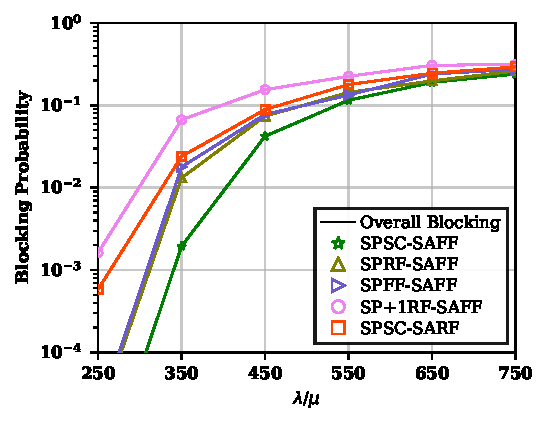
\includegraphics[width=\textwidth]{NSF_Single.pdf}
        \caption{}
        \label{fig:NSF_Single_Colored}
    \end{subfigure}
    \hfill
    \begin{subfigure}[b]{0.48\textwidth}
        \centering
        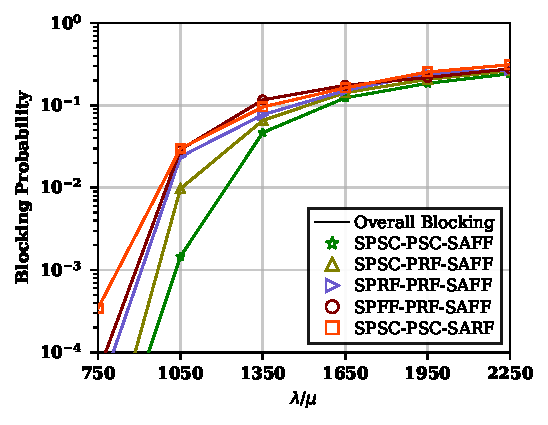
\includegraphics[width=\textwidth]{NSF_Parallel.pdf}
        \caption{}
        \label{fig:NSF_Parallel_Colored}
    \end{subfigure}
    \caption{$P_b$ vs Erlangs, holding time $1/\mu=60$s. Provisioning of the NSFNET topology spectral contention under (a) single-link and (b) 3$\times$ parallel-links.}
    \label{fig:nsf_topo}
\end{figure*}

\begin{figure*}[t]
    \centering
    \begin{subfigure}[b]{0.48\textwidth}
        \centering
        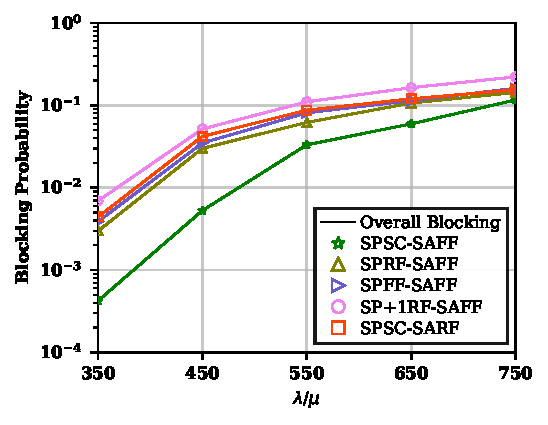
\includegraphics[width=\textwidth]{PAN_Single.pdf}
        \caption{}
        \label{fig:PAN_Single}
    \end{subfigure}
    \hfill
    \begin{subfigure}[b]{0.48\textwidth}
        \centering
        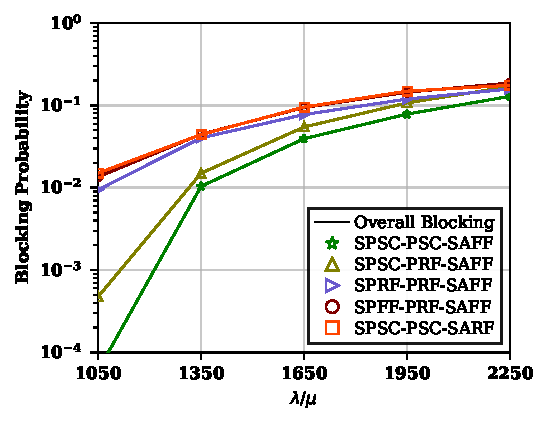
\includegraphics[width=\textwidth]{PAN_Parallel.pdf}
        \caption{}
        \label{fig:PAN_Parallel}
    \end{subfigure}
    \caption{$P_b$ vs Erlangs, holding time $1/\mu=60$s. Provisioning of the PANEU topology spectral contention under (a) single-link and (b) 3$\times$ parallel-links.}
    \label{fig:pan_topo}
\end{figure*}

Analysis as in Fig.~\ref{fig:nsf_topo}(a) of the NSFNET topology at~\emph{250} Erlangs reveals that the SPSC, SPRF, and SPFF schemes maintain a blocking probability below $10^{-4}$. Because network blocking is a rare event at this load, achieving stable results requires extended simulation periods~\footnote{Consequently, the results for the SPSC and SPRF schemes rely on confidence intervals of 48.38\% (with 32M requests) and 15.78\% (with 30M requests), respectively}. Notably, the SP+1 scheme is outperformed by standard shortest-path alternatives. This performance gap indicates that the inclusion of additional links increases total resource occupancy. Finally, applying the SARF policy to SPSC is confirmed to degrade blocking probability significantly. However, SPSC-SARF performs better than SP+1RF-SAFF, and this is because it checks all possible path combinations to maximize total capacity.

The system exhibits similar behavior under parallel configurations as in Fig.~\ref{fig:nsf_topo}(b). Total resource capacity increases by $3\times$ in these scenarios, and the performance scales predictably with a $3\times$ increase in network load. For the parallel expansion phase, the implementation utilizes a random-fit strategy, because first-fit allocation fails to exploit the full potential of multiple parallel links. The analysis compares two specific SPSC schemes, as SPSC introduces unavoidable computational latency. The latency of the SPSC-PRF-SAFF scheme is significantly better than that of SPSC-PSC-SAFF. Under these conditions, the SPSC-PSC-SAFF, SPSC-PRF-SAFF, and SPRF-PRF-SAFF schemes all maintain blocking probabilities below $10^{-4}$. Due to their inefficient resource occupancy, the SP+1 and SARF schemes are excluded from the parallel configuration analysis. After SPSC, the SPRF-PRF-SAFF scheme consistently maintains the second-best performance.

For the PANEU topology, network loads of 250 Erlangs in single-link mode as in Fig.~\ref{fig:pan_topo}(a) and 750 Erlangs in parallel-link mode as in Fig.~\ref{fig:pan_topo}(b) are insufficient to induce blocking. These test scenarios were subsequently excluded, as no blocking events occurred even with~\emph{30M requests}. When comparing topologies, the SPSC scheme in PANEU maintains a blocking probability between $10^{-3}$ and $10^{-4}$, whereas the NSFNET equivalent ranges between $10^{-2}$ and $10^{-3}$. The parallel configuration exhibits similar comparative behavior. Although the SPSC-PRF-SAFF scheme maintains higher blocking probabilities than the SPSC-PSC-SAFF variant, it remains highly efficient regarding latency. For official deployment, the SPSC scheme is recommended, as the latency is acceptable with $\geq 3\times$ parallel links. If real-world deployments require lower computational overhead, operators may prioritize the SPRF-PRF-SAFF scheme to improve performance.

\chapter{Conclusion and Future Work}
This concluding chapter summarizes the overarching achievements and technical contributions presented throughout this thesis. It critically reflects on the practical constraints and structural limitations encountered during the implementation phase and outlines potential avenues for future research to further refine the management of flexible-grid optical networks within TFS ecosystem.
\section{Summary of Contributions}
This thesis delivers a comprehensive end-to-end solution for the RSA problem in multi-fiber EONs, integrated directly into the TFS ecosystem. The work spans algorithm design, microservice engineering, device driver enhancement, and graphical interface development. Together, these contributions address the critical computational bottlenecks that arise when parallel fiber links introduce exponential path permutations and complex spectrum continuity constraints.

The central algorithmic contribution is a novel heuristic RSA approach purpose-built for topologies with non-uniform parallel links. The algorithm introduces a multi-directed graph abstraction technique that collapses parallel physical links into single logical edges, transforming the raw topology $G$ into a simplified graph $G_s$. This structural simplification reduces routing complexity from exponential to linear in the number of parallel links. Dijkstra's Shortest Path runs on $G_s$ to discover the primary route and additional candidate paths within a configurable hop-count tolerance $\mathcal{H} \leq \mathcal{H}_{min} + \Delta\mathcal{H}$. The selected node-level path is then expanded back onto the original multi-graph via an in-memory lookup table, recovering all parallel link combinations without re-traversing the full topology. For spectrum assignment, the algorithm maps endpoint frequency ranges to bitmaps where each bit represents a~\emph{12.5 GHz} Frequency Slot Unit, aligns heterogeneous ranges to a standardized reference, and performs a hop-by-hop bitwise intersection that identifies contiguous available slots---enforcing both spectrum continuity and contiguity in a single pass. Three path-selection schemes are evaluated: SPFF, SPRF, and a novel SPSC that selects candidate routes based on real-time spectrum availability rather than relying solely on topological ordering. Simulation results demonstrate that the SPSC scheme consistently achieves superior blocking performance, maintaining blocking probability below $10^{-4}$ at $250$ Erlangs.

To operationalize this algorithm, a dedicated \emph{ParallelOpticalController} (POC) microservice was engineered and deployed within TFS via Kubernetes. The POC operates as an independent, modular component that communicates with the \emph{ContextService}, \emph{DeviceService}, and \emph{ServiceService} through gRPC. Its internal architecture implements a three-phase computational pipeline---graph abstraction of the multi-fiber topology, optimal path selection, and bitmap-based spectrum assignment---organized across shared modules for ITU-T flex-grid specifications and graph operations, and a core engine that orchestrates bandwidth calculation, hop-by-hop intersection, and final provisioning.

Alongside the POC, the existing TFS \emph{OpenConfig} and \emph{OpenROADM} device drivers were significantly enhanced with a dynamically adaptable extraction technique. Rather than applying monolithic parsing rules, the improved drivers first identify the exact hardware model and then apply a device-specific filter profile, with a default fallback for uncharacterized equipment. This approach reliably extracts vendor-agnostic parameters including physical endpoint indexes, transport types, operational modes, and---most critically---the exact minimum and maximum frequency ranges per endpoint that the bitmap alignment step of the RSA algorithm requires.

The TFS Web User Interface was also comprehensively upgraded to present these complex internal states to network operators. The enhanced interface visualizes detailed device endpoint capabilities and capacity metrics, implements ITU-standard frequency mapping displaying optical bands and wavelength ranges, shows real-time spectrum slot availability distinguishing used from available FSUs, and provides comprehensive optical connectivity information for established multi-hop lightpaths.

All contributions were validated on a purpose-built distributed testbed comprising a primary server running MicroK8s-based TFS and a secondary server hosting Docker-based emulated muxponders and ROADMs configured with \emph{OpenConfig} and \emph{OpenROADM} YANG models. Evaluations were conducted on \emph{NSFNET} (14 nodes, up to 66 links with a $3\times$ parallel multiplier) and \emph{PANEU} (27 nodes, up to 165 links) topologies in both single-link and parallel-link configurations, demonstrating the algorithm's scalability and the system's end-to-end operational correctness.
\section{Limitations}
Integrating the POC adds significant capabilities to the TFS ecosystem, particularly in managing parallel links and visualizing spectrum allocation. However, the current framework operates within distinct structural boundaries. Broadly, these constraints fall into three categories: architectural dependencies, algorithmic assumptions, and device-level interactions.
\subsection{ Architectural Dependencies and Performance Overheads}
A fundamental limitation is that the POC operates as a stateful service. Ideally, microservices are engineered to be stateless and independent. However, this RSA engine is deeply integrated with the TFS control plane. It relies on continuous communication with the Context Service to fetch topology updates, optical configurations, and device data. While statefulness is common in centralized SDN architectures, it tightly couples the controller to the specific TFS database schema. This dependency limits standalone portability and introduces computational latency. Currently, the system must perform numerous database queries to extract endpoint indexes, channel mappings, and flex-grid bitmaps. In highly scaled networks with dense parallel links, this frequent querying increases processing times, which could ultimately slow down real-time provisioning.
\subsection{ Algorithmic and Topological Assumptions}
The algorithmic approach to graph modeling and path discovery introduces several operational constraints. First, the NetworkX graph construction ($G$ and $G_s$) fundamentally assumes that all optical links are bi-directional. The Dijkstra-based shortest path and parallel path expansion algorithms compute routing metrics based on this symmetry. If the physical infrastructure contains uni-directional optical fibers or asymmetric spectrum availability, the current algorithmic formulation will fail to discover a valid end-to-end lightpath.

Secondly, the algorithm does not consider the internal cross-connections of a ROADM device. Because it relies strictly on peripheral device port-mappings, the model assumes that all degrees (DEGs) are fully interconnected without internal blocking or architectural interference. Finally, the algorithm utilizes deterministic values for routing path weight, modulation formats, and signal-to-noise ratios (SNR). Consequently, the number of FSUs required for each target bitrate is predefined within the algorithm rather than being calculated dynamically.
\subsection{ Performance Limitation of the Path Computation }
Although the path computation phase supports several path selection schemes, the final implementation utilizes the~\emph{SPSC}. SPSC marginally degrades overall throughput performance when the network topology is significantly large and dense. However, testing across two standard topologies demonstrated that SPSC still operates within acceptable performance delays. For networks more complex or dense than PANEU or NSFNET, it is advisable to evaluate the~\emph{SPRF} method alongside SPSC to determine the optimal solution.
\subsection{ Lifecycle Management and Device-Level Interactions}
From an operational lifecycle perspective, the current framework focuses primarily on the establishment of optical intents. The slot acquisition process currently requires manual intervention and intuitive oversight by the network operator. More importantly, the controller does not natively support an automated lightpath teardown and slot release mechanism. Once slots are marked as \texttt{IN\_USE} in the spectrum bitmap, reversing this hash to free the contiguous slots upon intent deletion requires manual reconciliation. Additionally, while the RSA algorithm successfully computes the path and updates the logical SDN database, it lacks the southbound provisioning logic to actively push the configurations down to the physical devices. Currently, the solution remains fully analytical and logical within the SDN control plane.
\section{Ongoing Official Contribution}
Since this work has been partially supported by external authorities~\footnote{This work has been partially supported by: National Inter-University Consortium for Telecommunications (CNIT), the Chips Joint Undertaking (JU), European Union (EU) HORIZON-JU-IA, under GA No. 101140087 (SMARTY); the EU Horizon Europe research and innovation program, ALLEGRO Project, under GA No. 101092766; the Italian Ministry of Education and Research (MUR) in the frame-work of the FoReLab project (Departments of Excellence).} an official version is ongoing and expected to be released in the upcoming versions of TFS. A few limitations such as: uni-directional link support, integration of~\emph{GNPy} to remove deterministic QoT metrics, and southbound interface integration to update physical devices.
\section{Future Work Directions}
Future research can be prioritized on comprehensive field testing to validate the proposed optical controller within live physical hardware environments. Furthermore, subsequent studies should investigate the architectural depth of expansive multi-fiber topologies, which inherently feature exponential routing options. This specific structural analysis will identify the precise computational trade-off point where the SPSC scheme mathematically benefits from parallel computation. Finally, the system requires the advanced integration of Artificial Intelligence to establish intelligent closed-loop automation. This cognitive enhancement will enable the network to continuously analyze dynamic telemetry data, and it will facilitate fully autonomous, intent-driven optical orchestration.
\clearpage
\addcontentsline{toc}{chapter}{Bibliography}
\printbibliography
\end{document}